\documentclass[conference]{IEEEtran}
\IEEEoverridecommandlockouts
%Template version as of 6/27/2024

% \usepackage{xcolor}
\usepackage[table,usenames,dvipsnames]{xcolor}

\usepackage{amsmath,amssymb,amsfonts}
\usepackage{graphicx}

\usepackage{nameref}

% For abbreviations, we use "acro" package, and mfirstuc to help capitalize long
% versions normally
\usepackage{mfirstuc}
\MFUhyphentrue % tell mfirstuc to capitalize hyphenated words

% Acronyms
\usepackage{acro}
% For one-offs,
% \DeclareAcronym{acronym}{short=short-version,long=long-version}

\newcommand{\newacr}[2]{\DeclareAcronym{#1}{short=\uppercase{#1},long=#2}}
\newcommand{\newacrs}[3]{\DeclareAcronym{#1}{short=#2,long=#3}}

% Alphabetically sorted list of acronyms
\newacr{aop}{Aspect-Oriented Programming}
\newacr{api}{Application Programming Interface}
\newacr{ast}{Abstract Syntax Tree}
\newacr{cms}{Content Management System}
\newacr{cpu}{Central Processing Unit}
\newacr{csv}{Comma-Separated Values}
\newacr{dsl}{Domain-Specific Language}
\newacr{ffi}{Foreign Function Interface}
\newacr{gui}{Graphical User Interface}
\newacr{html}{HyperText Markup Language}
\newacr{href}{Hypertext REFerence}
\newacr{ide}{Integrated Development Environment}
\newacr{json}{JavaScript Object Notation}
\newacr{jvm}{Java Virtual Machine}
\newacr{mop}{MetaObject Protocol}
\newacr{nasa}{National Aeronautics and Space Administration}
\newacr{pdf}{Portable Document Format}
\newacr{sst}{Skeleton Syntax Tree}
\newacr{wysiwyg}{What You See Is What You Get}

% Case Studies 
%   (note: I'm grouping these together and forcing "newacrs" usage, even when
%    seemingly unneeded because, otherwise, they won't group together at the 
%    bottom of the complete "acronyms" list.)
\newacrs{glassbr}{GlassBR}{Glass Breaking}
\newacrs{projectile}{Projectile}{Projectile}
\newacrs{sglpend}{SglPend}{Single Pendulum}
\newacrs{dblpend}{DblPend}{Double Pendulum}
\newacrs{gamephysics}{GamePhysics}{Game Physics}
\newacrs{hghc}{HGHC}{Heat Transfer Coefficients between Fuel and Cladding in Fuel Rods}
\newacrs{pdcontroller}{PDController}{Proportional Derivative Controller}
\newacrs{swhs}{SWHS}{Solar Water Heating System}
\newacrs{nopcm}{SWHSNoPCM}{Solar Water Heating System Without PCM}
\newacrs{ssp}{SSP}{Slope Stability analysis Program}


%------------------------------------------------------------------------------
%- Extra commands for more functionality -- in particular, capitalizing the
%- long form of acronyms.
%------------------------------------------------------------------------------

% Defining \ACL - to capitalize all words in an acronym
% Credits to: https://tex.stackexchange.com/a/257896
\NewDocumentCommand\ACF{sm}{%
  \begingroup
  \acsetup{uppercase/cmd=\ecapitalisewords}%
  \IfBooleanTF{#1}{\Acf*{#2}}{\Acf{#2}}%
  \endgroup
}

\NewDocumentCommand\ACFP{sm}{%
  \begingroup
  \acsetup{uppercase/cmd=\ecapitalisewords}%
  \IfBooleanTF{#1}{\Acfp*{#2}}{\Acfp{#2}}%
  \endgroup
}

\NewDocumentCommand\ACL{sm}{%
  \begingroup
  \acsetup{uppercase/cmd=\ecapitalisewords}%
  \IfBooleanTF{#1}{\Acl*{#2}}{\Acl{#2}}%
  \endgroup
}

\NewDocumentCommand\ACLP{sm}{%
  \begingroup
  \acsetup{uppercase/cmd=\ecapitalisewords}%
  \IfBooleanTF{#1}{\Aclp*{#2}}{\Aclp{#2}}%
  \endgroup
}


% General Assets
%------------------------------------------------------------------------------
% Code
%------------------------------------------------------------------------------

\input{assets/code/names}
\input{assets/misc/posterHelpers}

% for assets/code/example.tex...
\newcommand{\exampleCode}{\input{assets/code/example}}
\newcommand{\refExampleCode}{\Cref{lst:exampleCode}}

% for assets/code/examplePseudocode.tex...
\newcommand{\examplePseudocode}{\input{assets/code/examplePseudocode}}
\newcommand{\refExamplePseudocode}{\Cref{lst:examplePseudocode}}

% for assets/code/mainInvalidInputTest.tex...
\newcommand{\mainInvalidInputTest}{\input{assets/code/mainInvalidInputTest}}
\newcommand{\refMainInvalidInputTest}{\Cref{lst:mainInvalidInputTest}}

% for assets/code/projManualViolationReq.tex...
\newcommand{\projManualViolationReq}{\input{assets/code/projManualViolationReq}}
\newcommand{\refProjManualViolationReq}{\Cref{lst:projManualViolationReq}}

% for assets/code/projViolationChoice.tex...
\newcommand{\projViolationChoice}{\input{assets/code/projViolationChoice}}
\newcommand{\refProjViolationChoice}{\Cref{lst:projViolationChoice}}

%------------------------------------------------------------------------------
% Graphs
%------------------------------------------------------------------------------

% Organization of files

\newcommand{\parChdGraphs}{
    % Only top or bottom to comply with IEEE guidelines
    \begin{figure}[bt!]
        \centering
        \begin{subfigure}[b]{\linewidth}
            \centering
            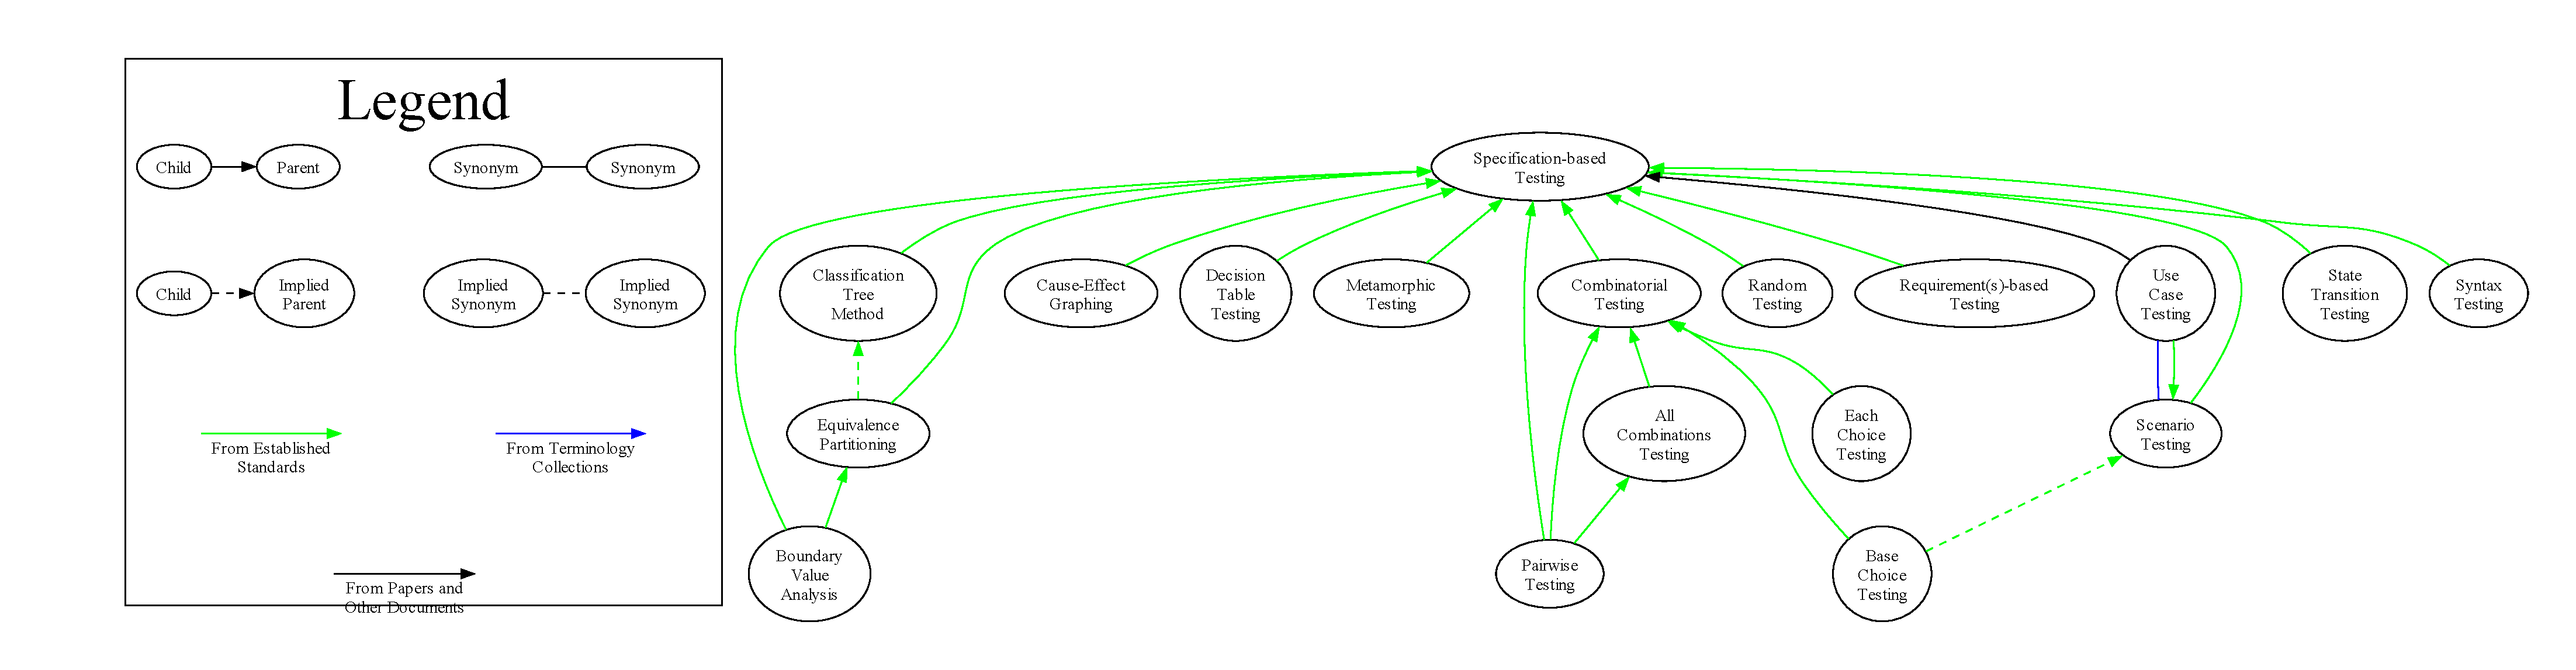
\includegraphics[width=\linewidth]{assets/graphs/specBasedGraph.pdf}
            \caption{``Superset'' relations.}
            \label{fig:specBasedGraph}
        \end{subfigure}
        \begin{subfigure}[t]{.45\linewidth}
            \centering
            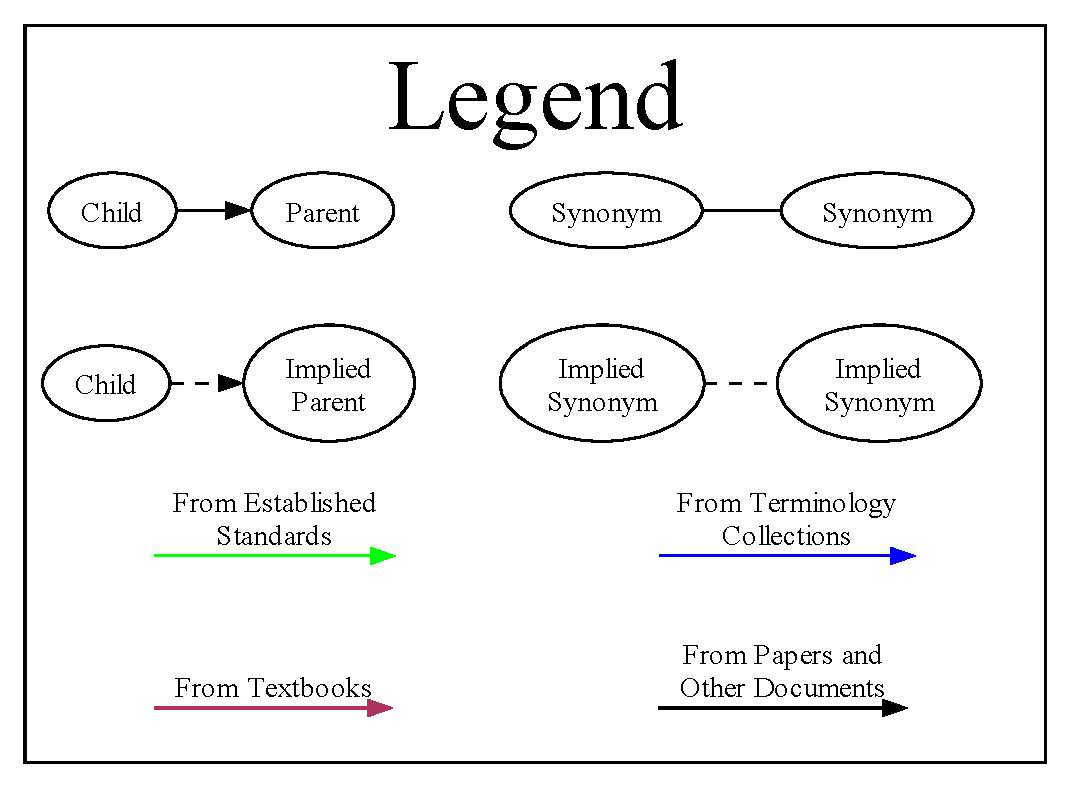
\includegraphics[width=\linewidth]{assets/graphs/parChdLegend.pdf}
        \end{subfigure}
        \begin{subfigure}[t]{.5\linewidth}
            \centering
            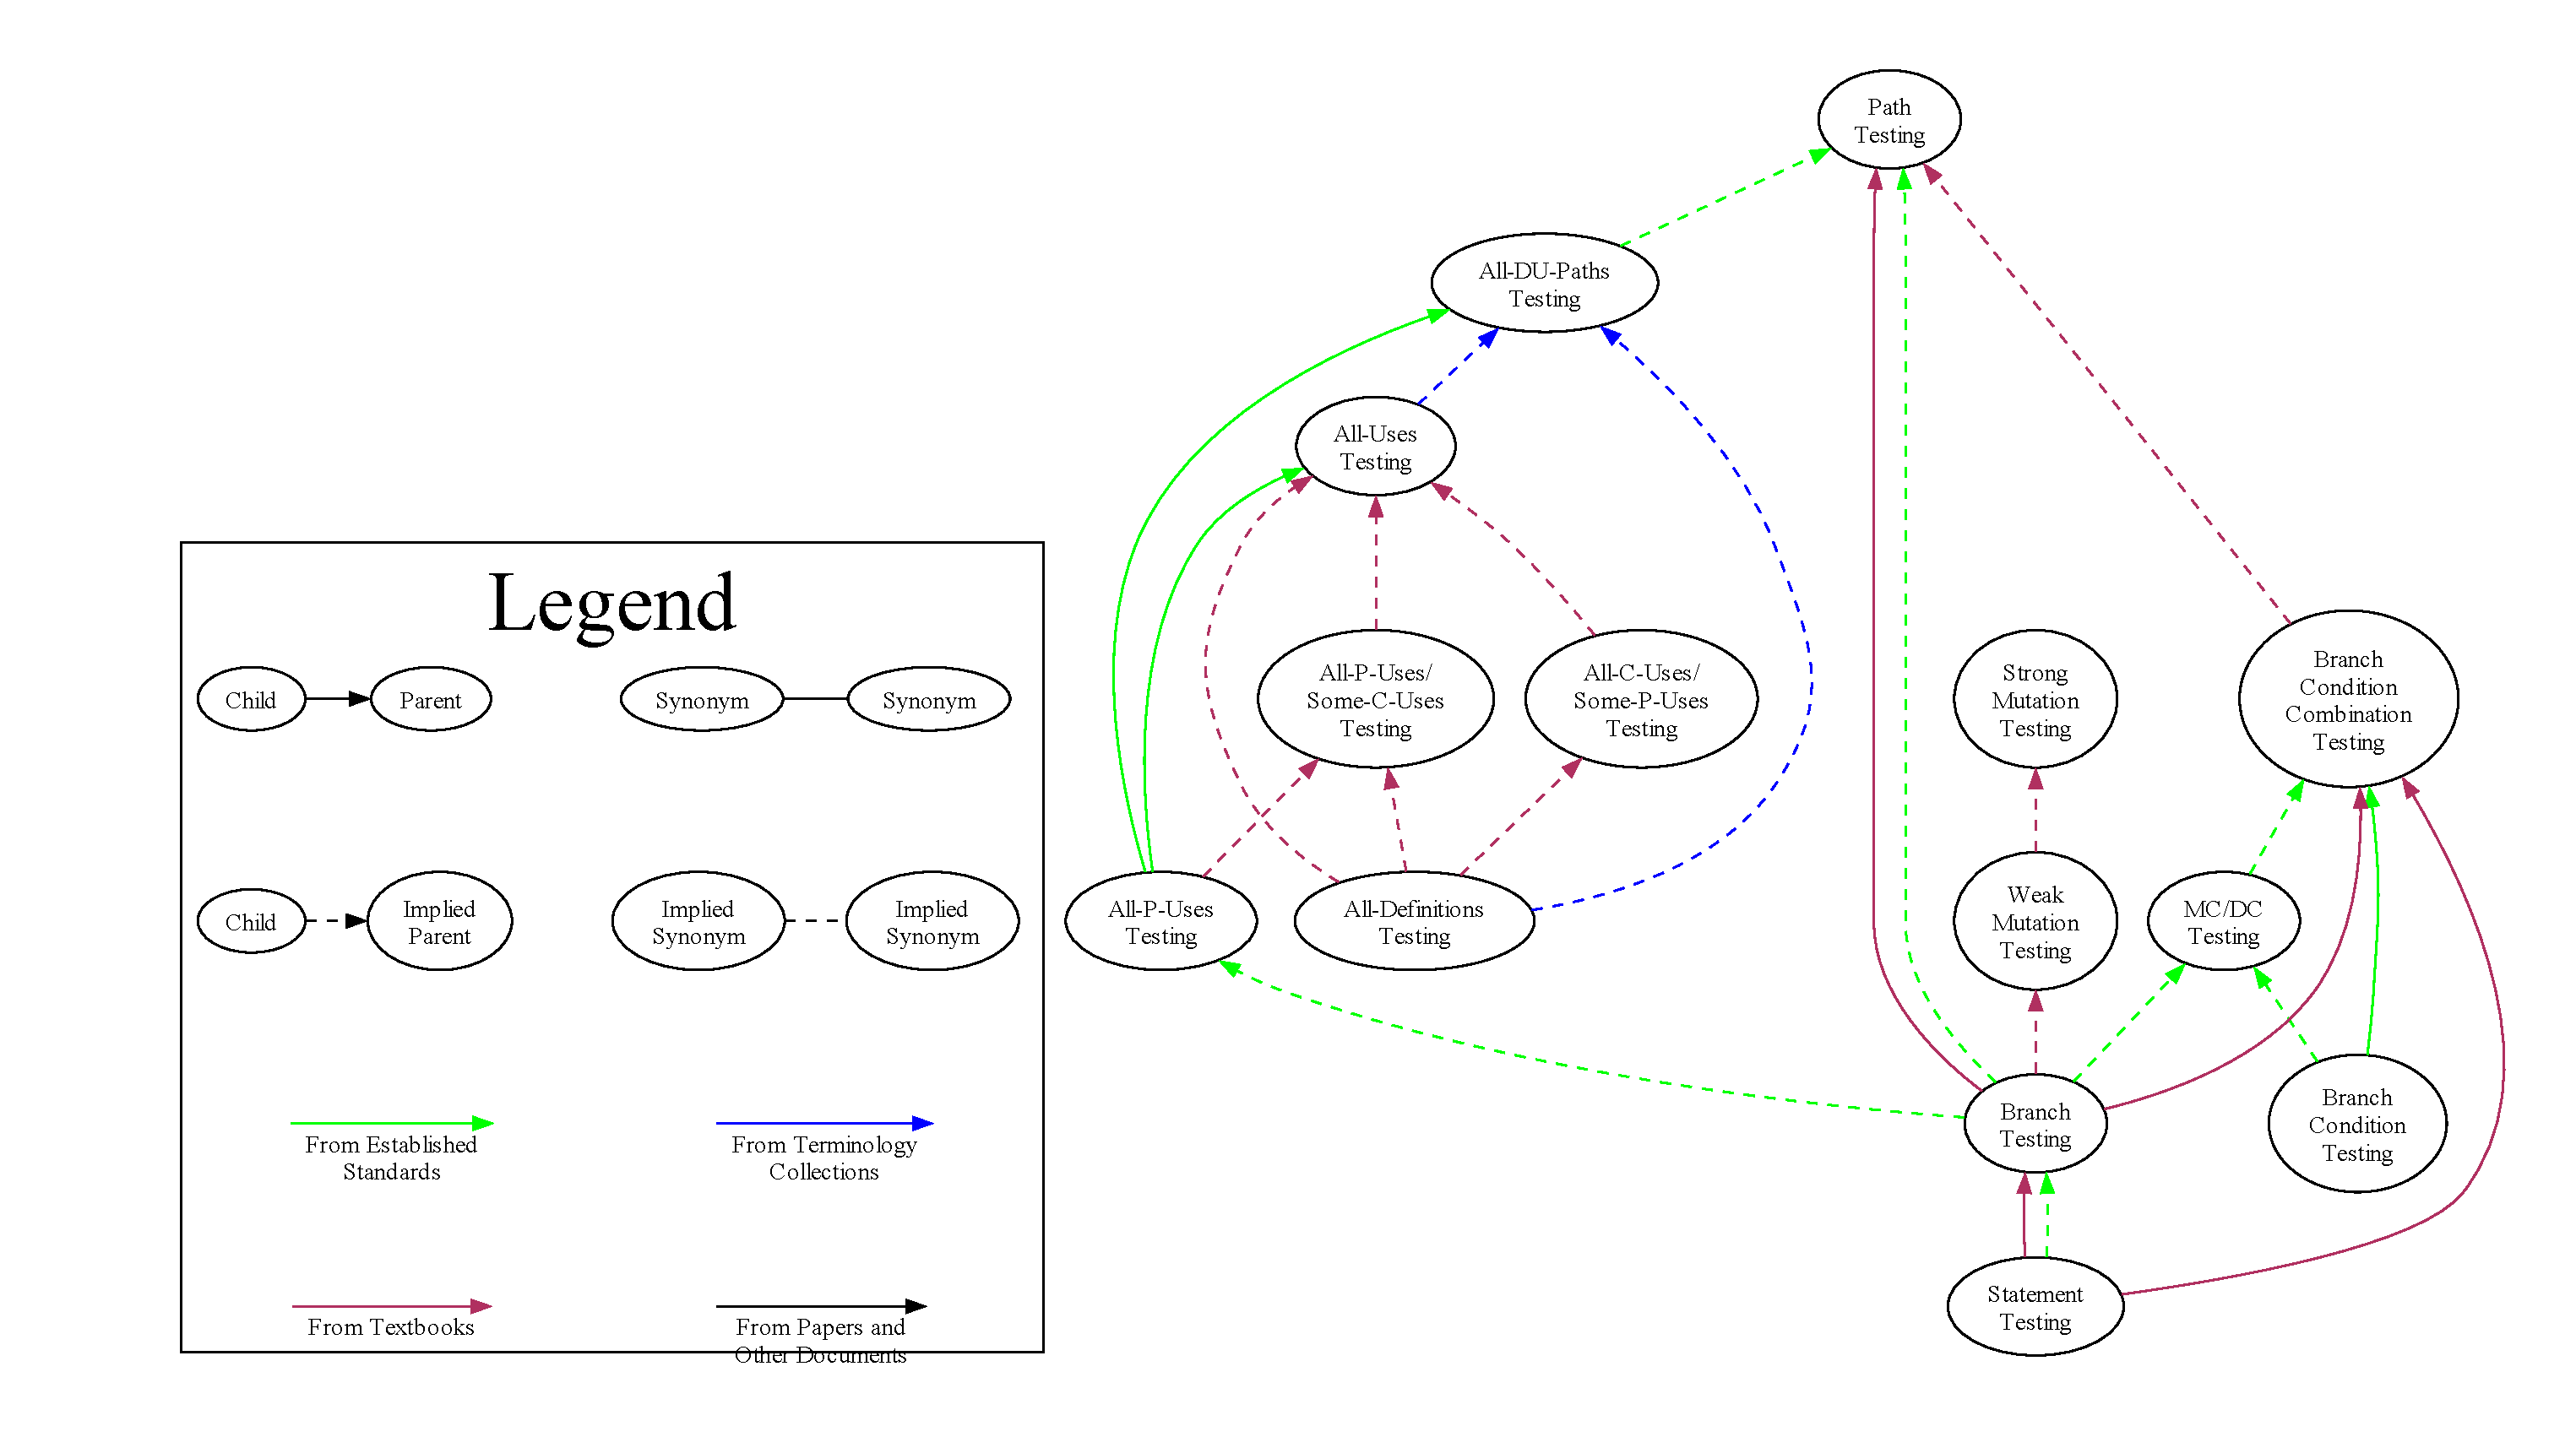
\includegraphics[width=\linewidth]{assets/graphs/subsumesGraph.pdf}
            \caption{``Subsume'' relations.}
            \label{fig:subsumesGraph}
        \end{subfigure}
        \caption{Graphs of different classes of \hyperref[par-chd-rels]{parent-child relations}.}
        \label{fig:parChdGraphs}
    \end{figure}
}

\newcommand{\ExampleGraph}{
    \begin{figure*}
        \begin{subfigure}[b]{0.3\linewidth}
            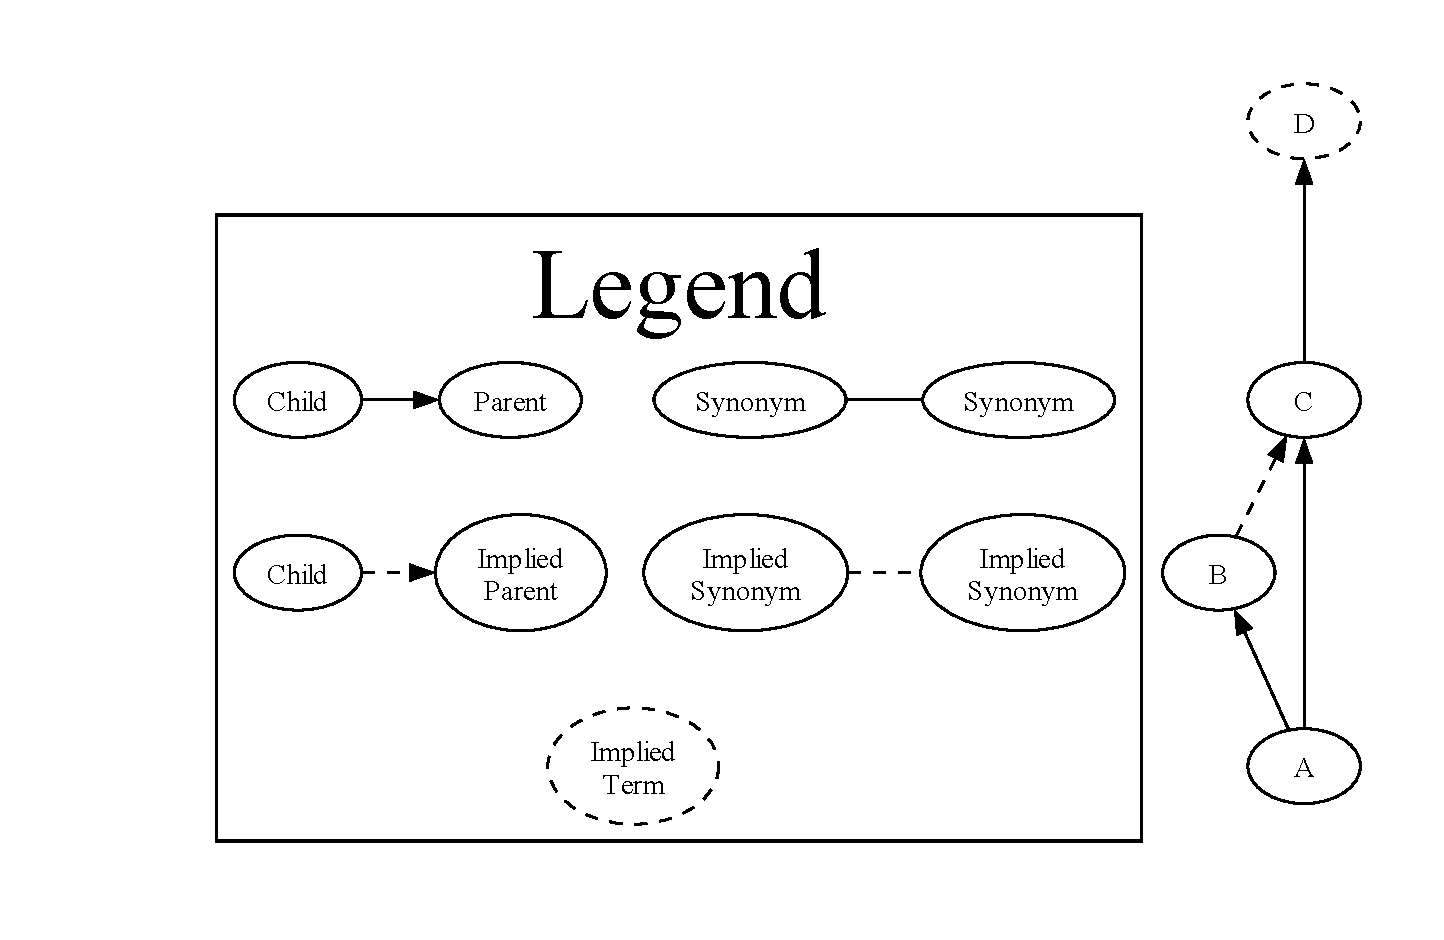
\includegraphics[width=\linewidth]{assets/graphs/ExampleGlossaryGraph.pdf}
            \caption{Graph from \Cref{tab:exampleGlossary}.}
            \label{fig:exampleGraph}
        \end{subfigure}
        \centering
        \begin{subfigure}[b]{0.675\linewidth}
            \centering
            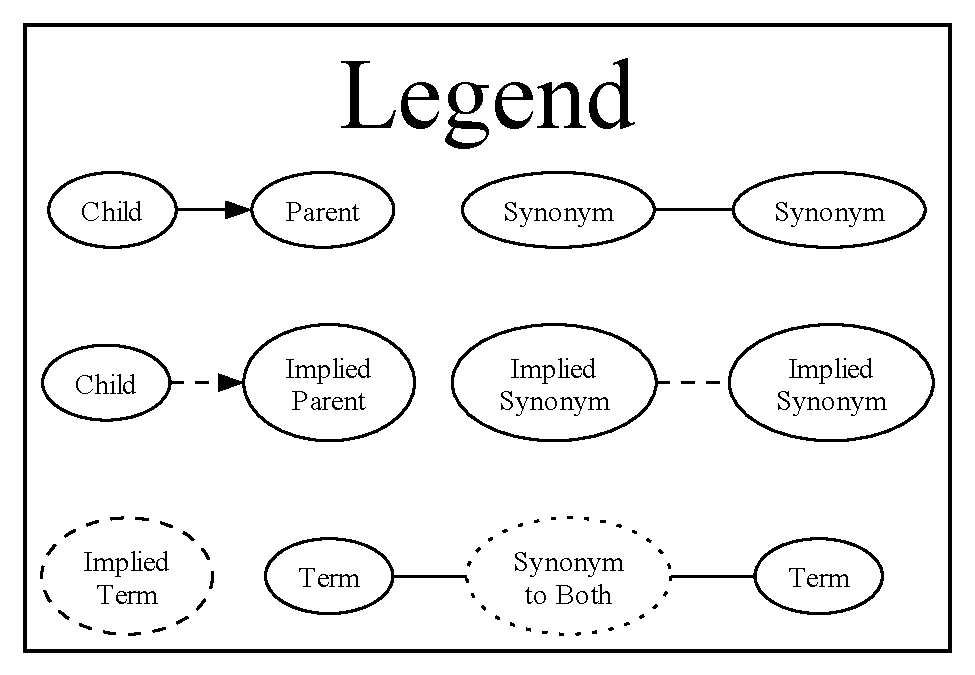
\includegraphics[width=0.8\linewidth]{assets/graphs/manual/manualLegendNonSolidTerms.pdf}
            \hspace{5cm}\begin{subfigure}[t]{0.475\linewidth}
                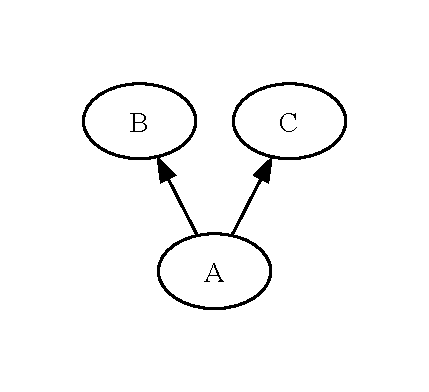
\includegraphics[width=1.1\linewidth]{assets/graphs/rigidExampleGlossaryGraph.pdf}
                \caption{Rigid graph from\\\Cref{tab:exampleGlossary}.}
                \label{fig:rigidExampleGraph}
            \end{subfigure}
            \begin{subfigure}[t]{0.475\linewidth}
                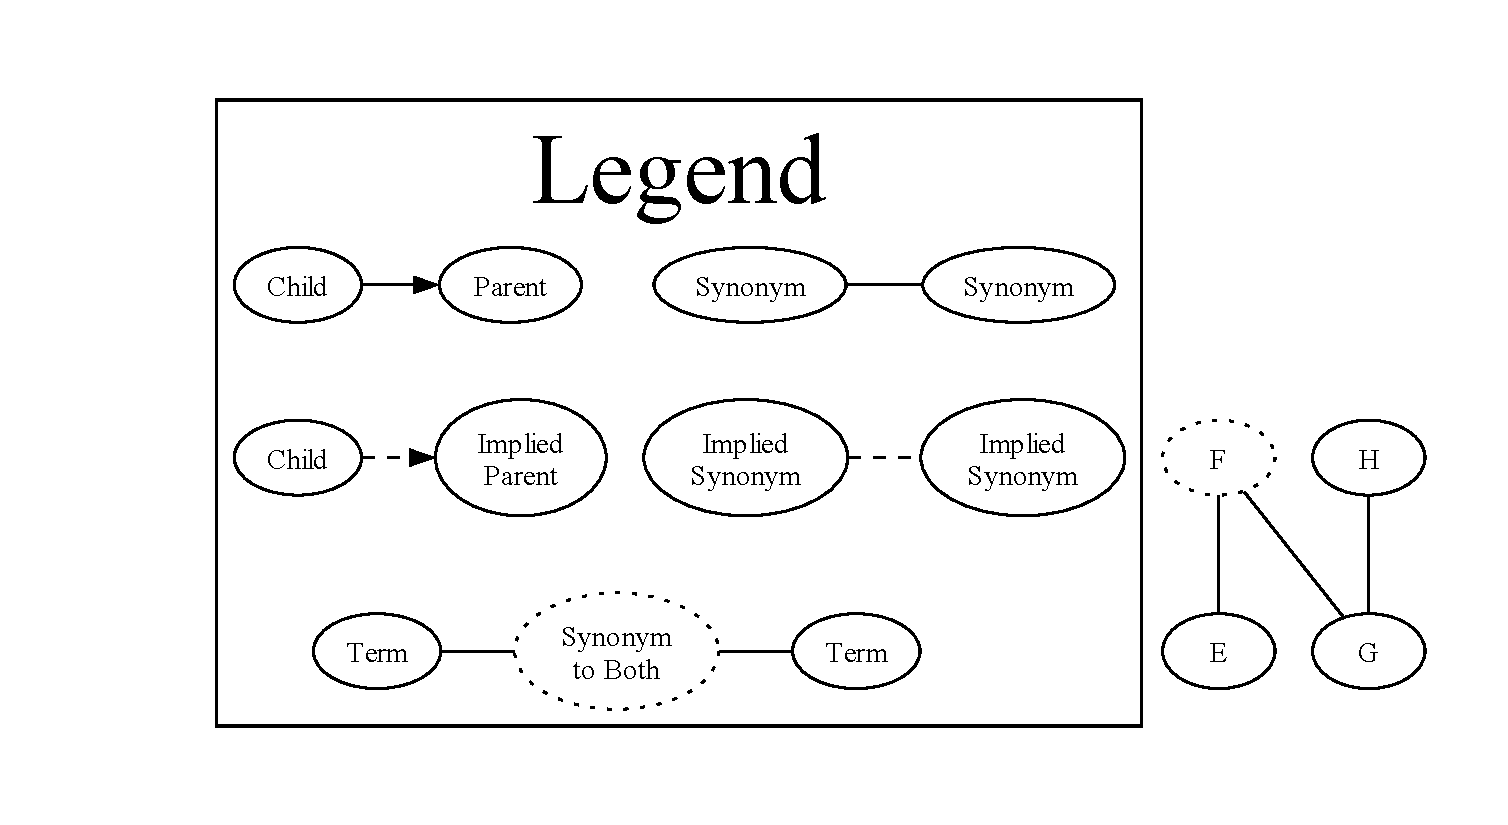
\includegraphics[width=1.1\linewidth]{assets/graphs/SynExampleGlossaryGraph.pdf}
                \caption{Graph from \Cref{tab:synExampleGlossary}.}
                \label{fig:synExampleGraph}
            \end{subfigure}
        \end{subfigure}
        \begin{subfigure}[t]{0.25\linewidth}
            \centering
            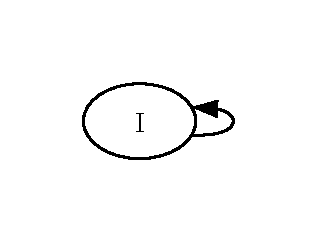
\includegraphics[width=1.2\linewidth]{assets/graphs/SelfExampleGlossaryGraph.pdf}
            \caption{Self-loop graph.}
            \label{fig:selfExampleGraph}
        \end{subfigure}
        \hfill
        \begin{subfigure}[t]{0.425\linewidth}
            \centering
            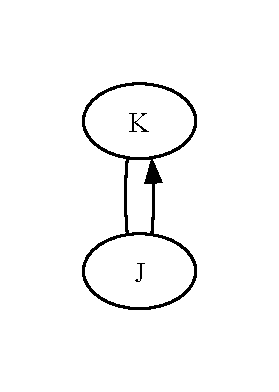
\includegraphics[width=0.6\linewidth]{assets/graphs/ParSynExampleGlossaryGraph.pdf}
            \caption{Graph of a pair of terms with a \hyperref[par-chd-rels]{parent-child} \emph{and} synonym relation.}
            \label{fig:parSynExampleGraph}
        \end{subfigure}
        \hfill
        \begin{subfigure}[t]{0.25\linewidth}
            \centering
            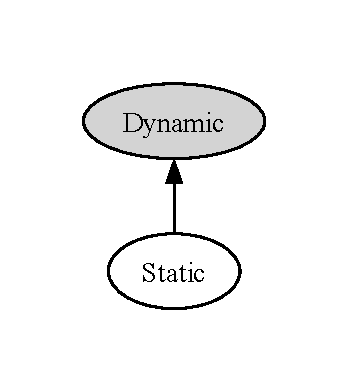
\includegraphics[width=1.4\linewidth]{assets/graphs/StaticExampleGlossaryGraph.pdf}
            \caption{Static graph.}
            \label{fig:staticExampleGraph}
        \end{subfigure}
        \caption{Example generated graphs.}
        \label{fig:exampleGraphs}
    \end{figure*}
}

\newcommand{\recoveryGraphs}{
    % Only top or bottom to comply with IEEE guidelines
    \begin{figure}[bt!]
        \centering
        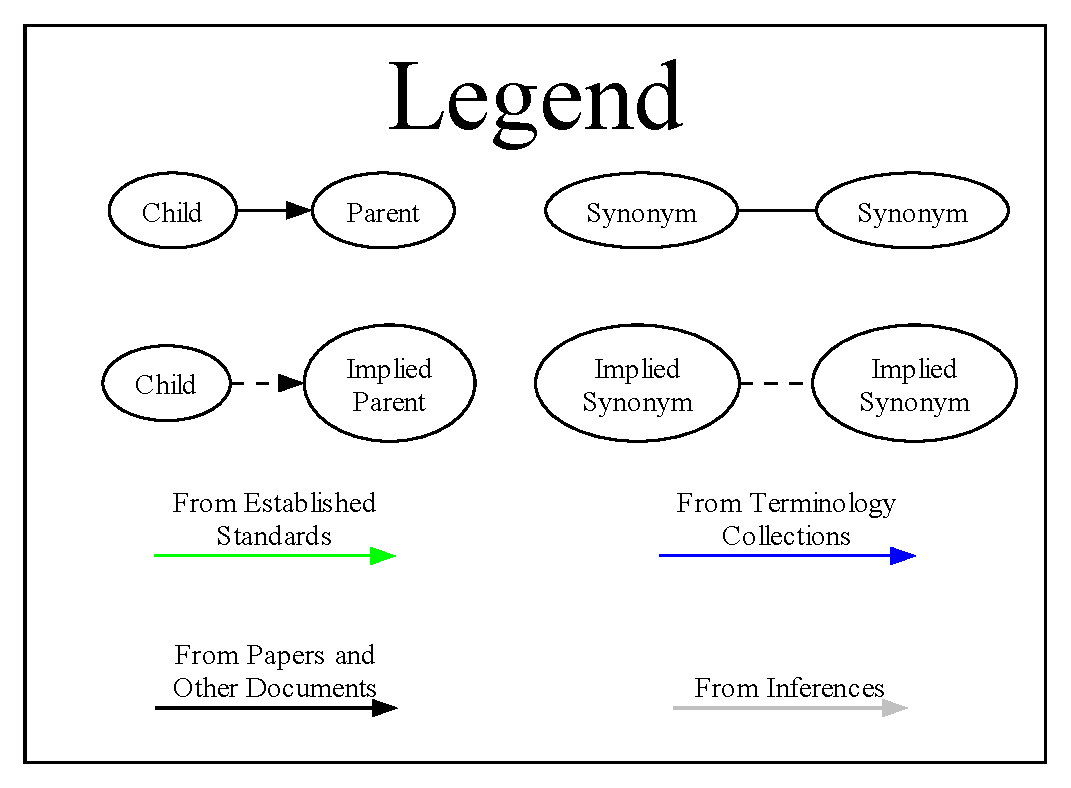
\includegraphics[width=\linewidth]{assets/graphs/recoveryLegend.pdf}
        \begin{subfigure}[b]{.55\linewidth}
            \centering
            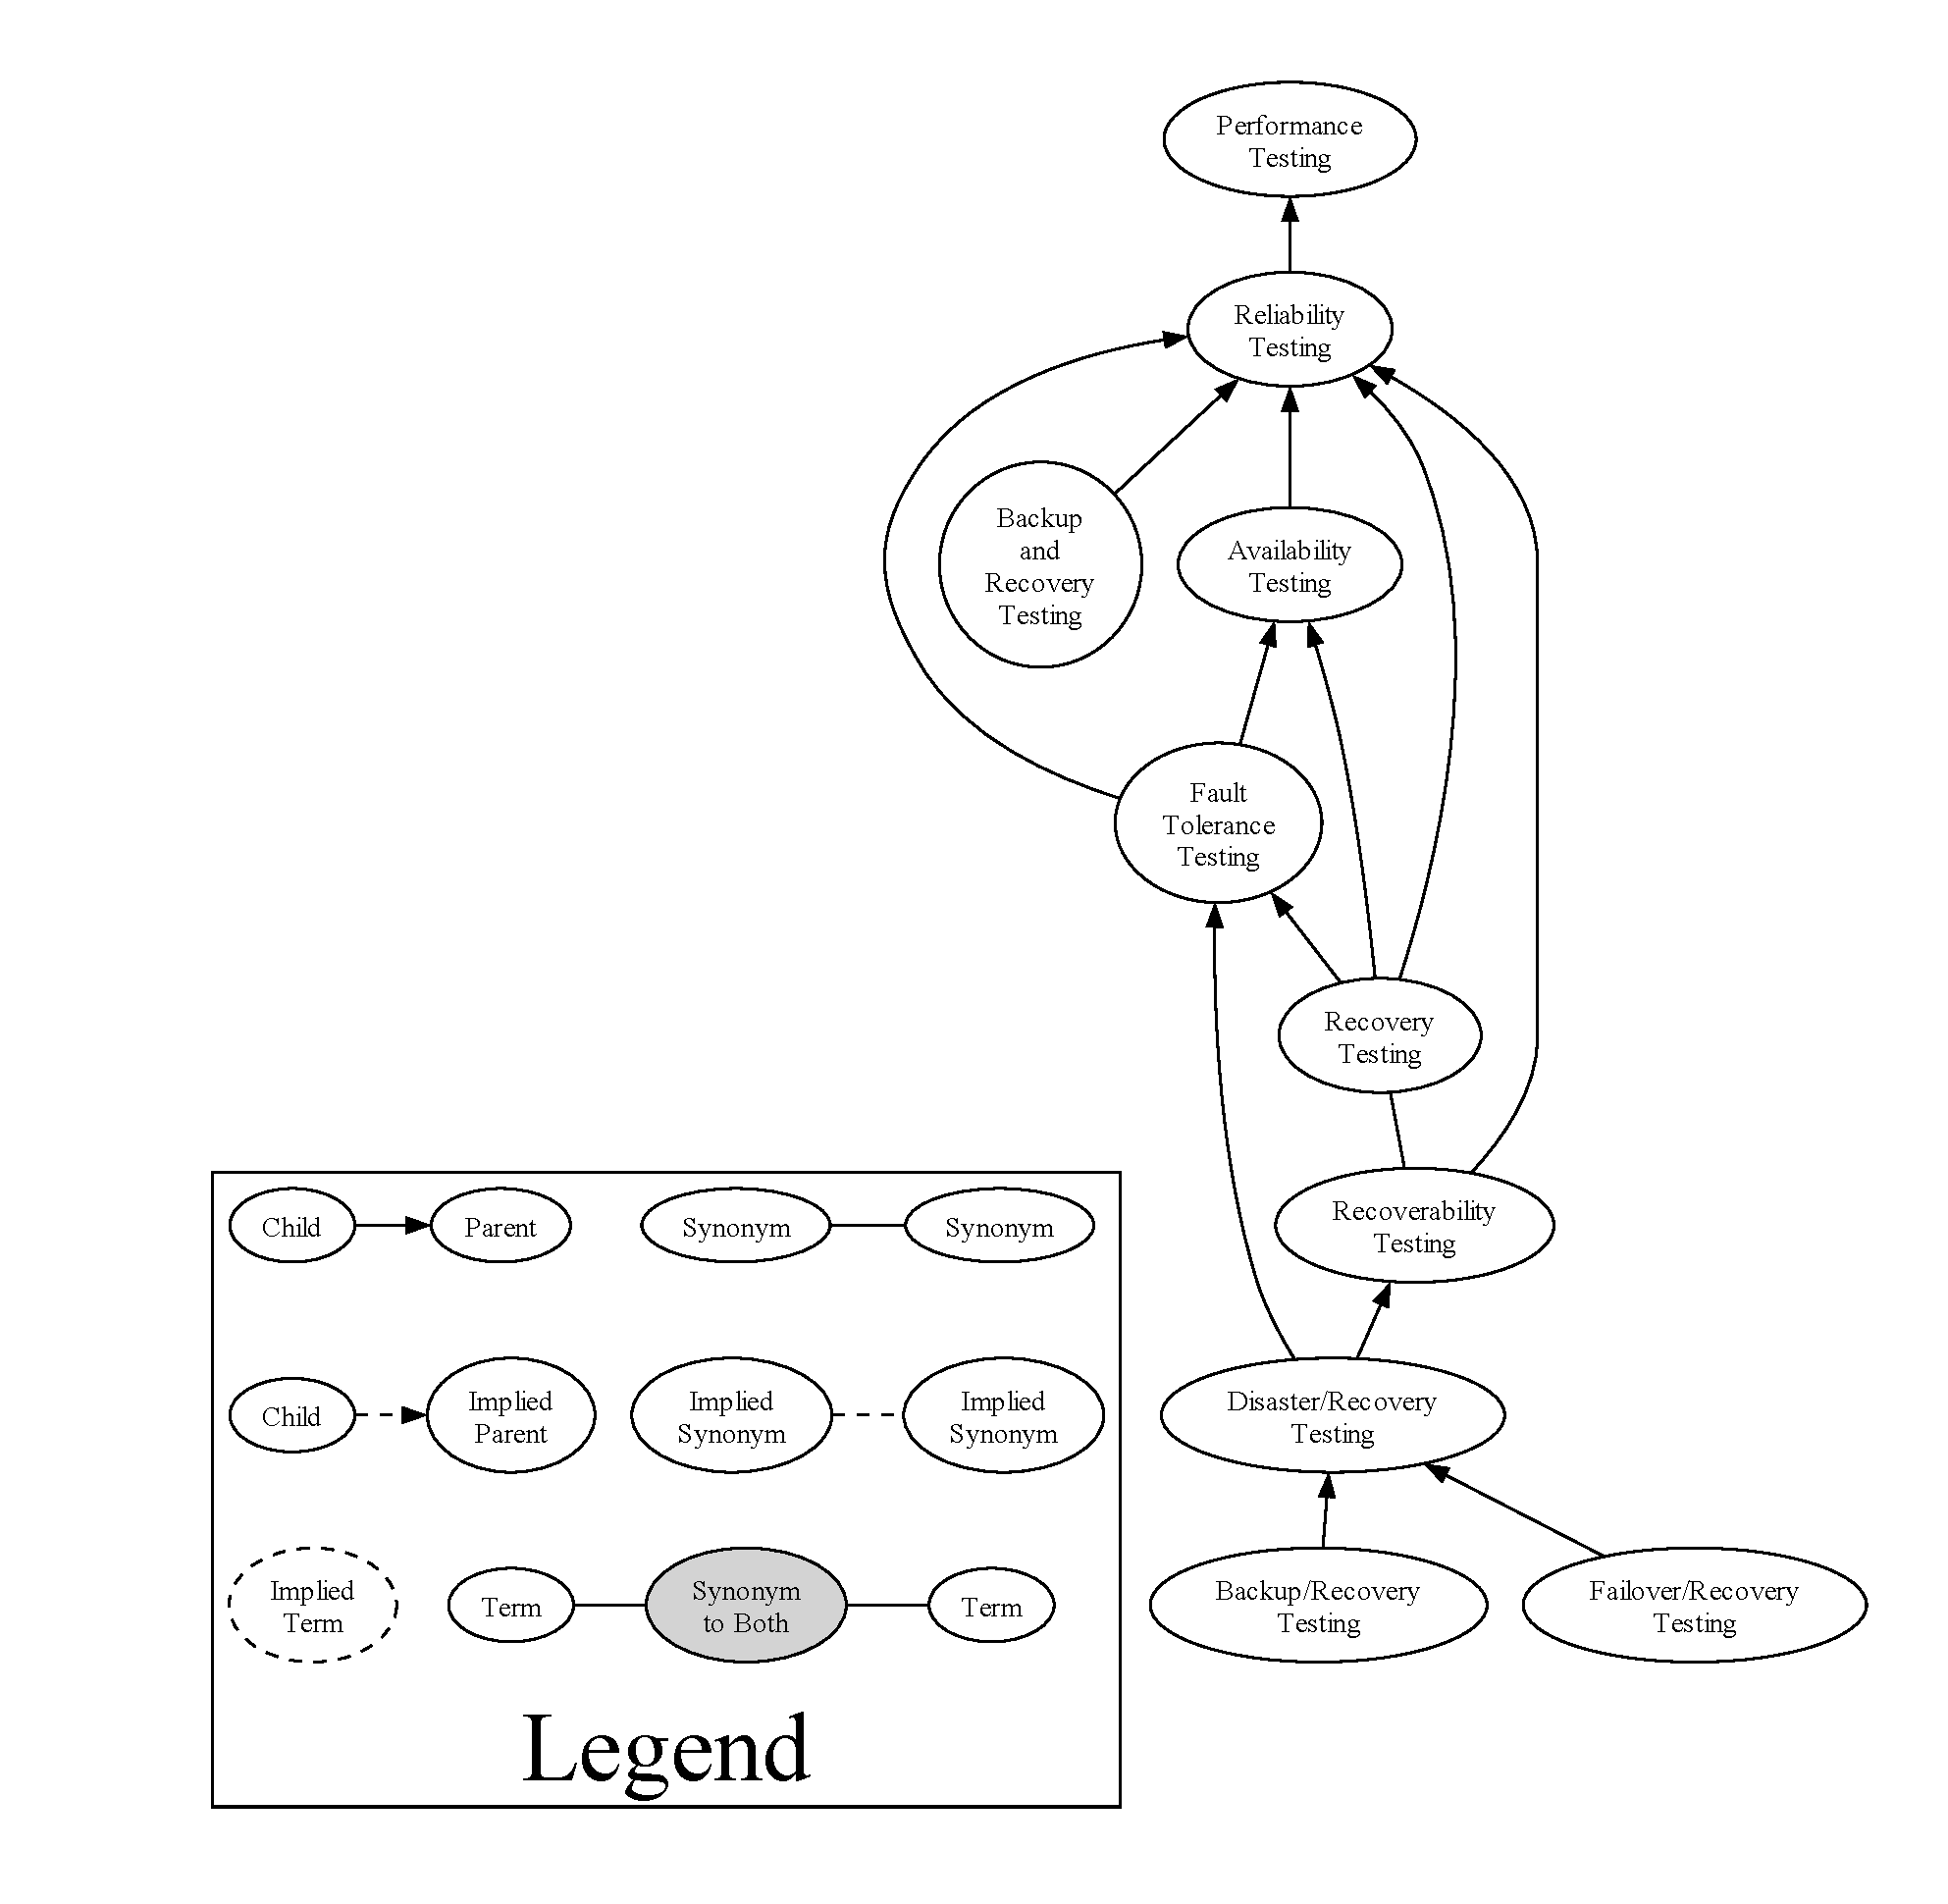
\includegraphics[width=\linewidth]{assets/graphs/recoveryGraph.pdf}
            \caption{Graph of current relations.}
            \label{fig:recovery-graph-current}
        \end{subfigure}
        \begin{subfigure}[b]{.4\linewidth}
            \centering
            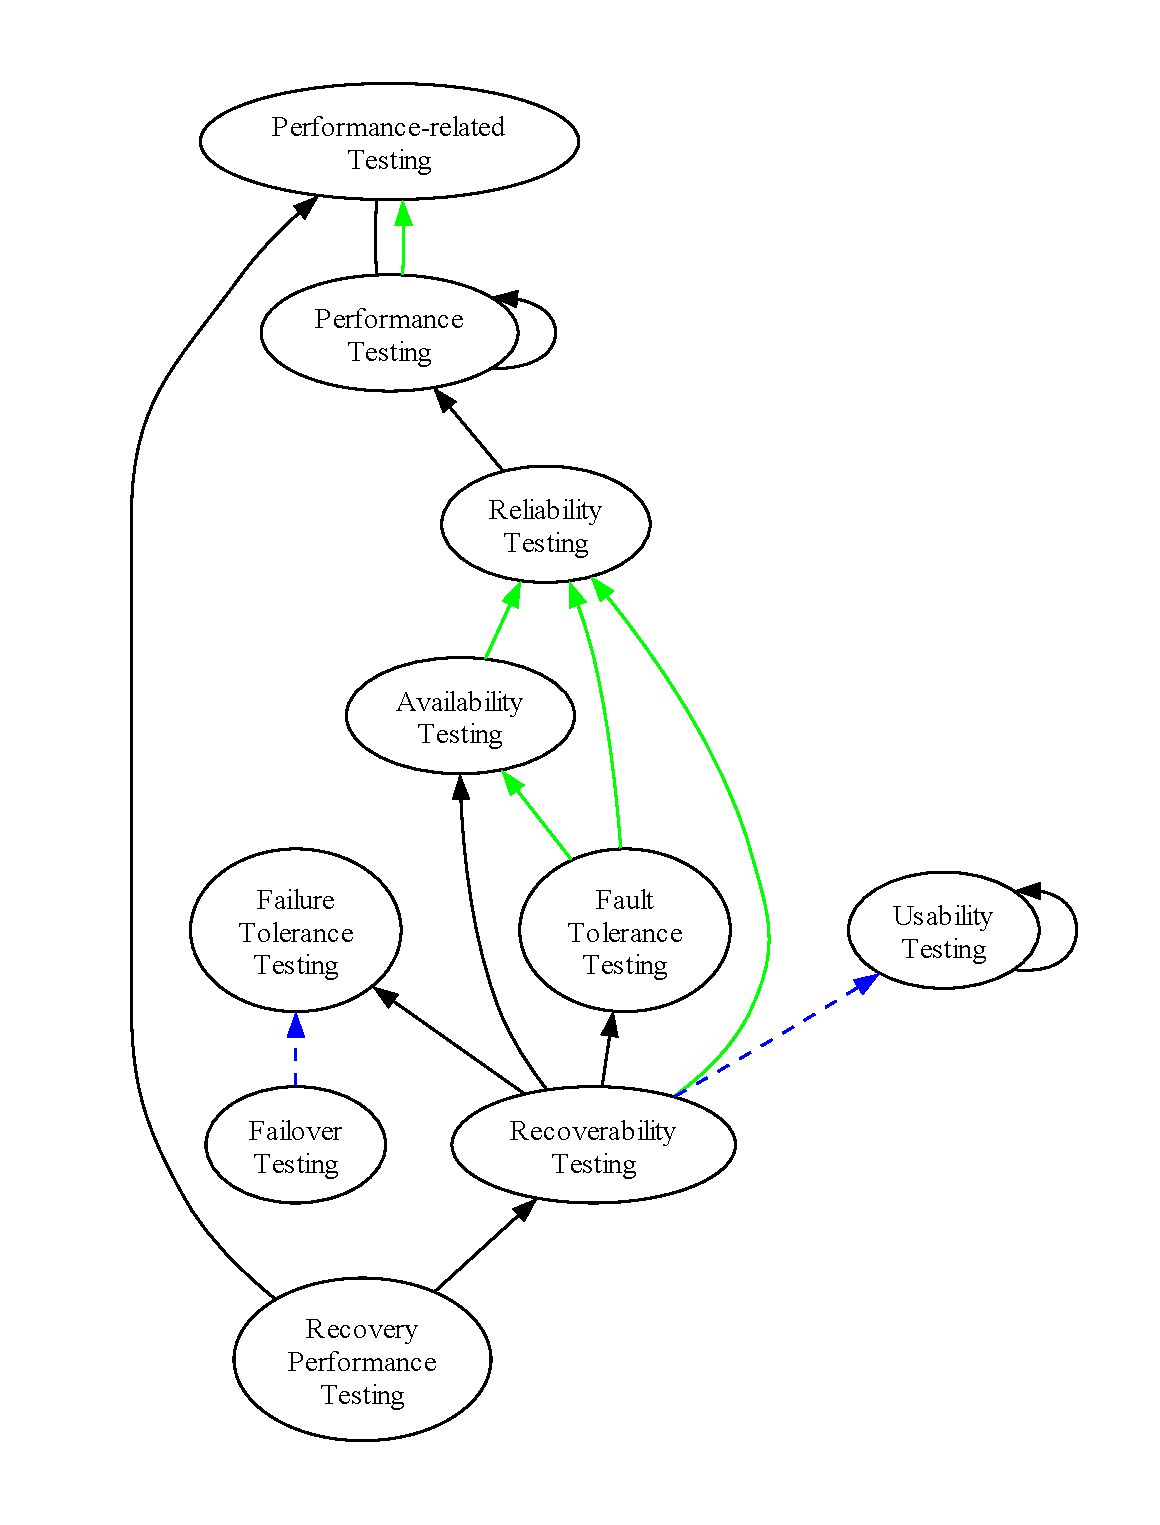
\includegraphics[width=\linewidth]{assets/graphs/recoveryProposedGraph.pdf}
            \caption{Graph of proposed relations.}
            \label{fig:recovery-graph-proposed}
        \end{subfigure}
        \caption{Graphs of relations between terms related to recovery testing.}
        \label{fig:recoveryGraphs}
    \end{figure}
}

\newcommand{\scalGraphs}{
    % Only top or bottom to comply with IEEE guidelines
    \begin{figure}[bt!]
        \centering
        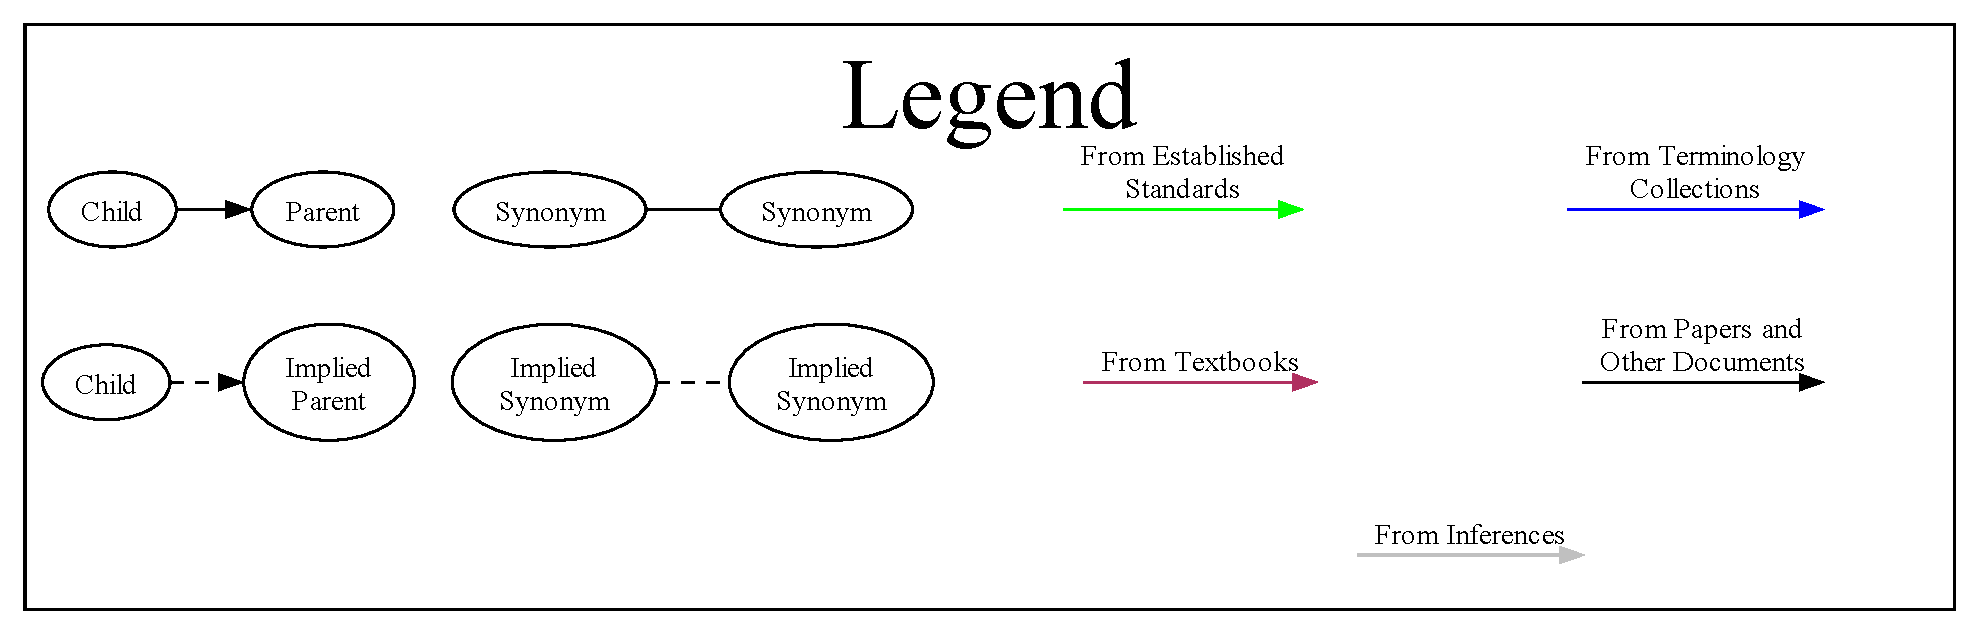
\includegraphics[width=\linewidth]{assets/graphs/scalabilityLegend.pdf}
        \begin{subfigure}[b]{.475\linewidth}
            \centering
            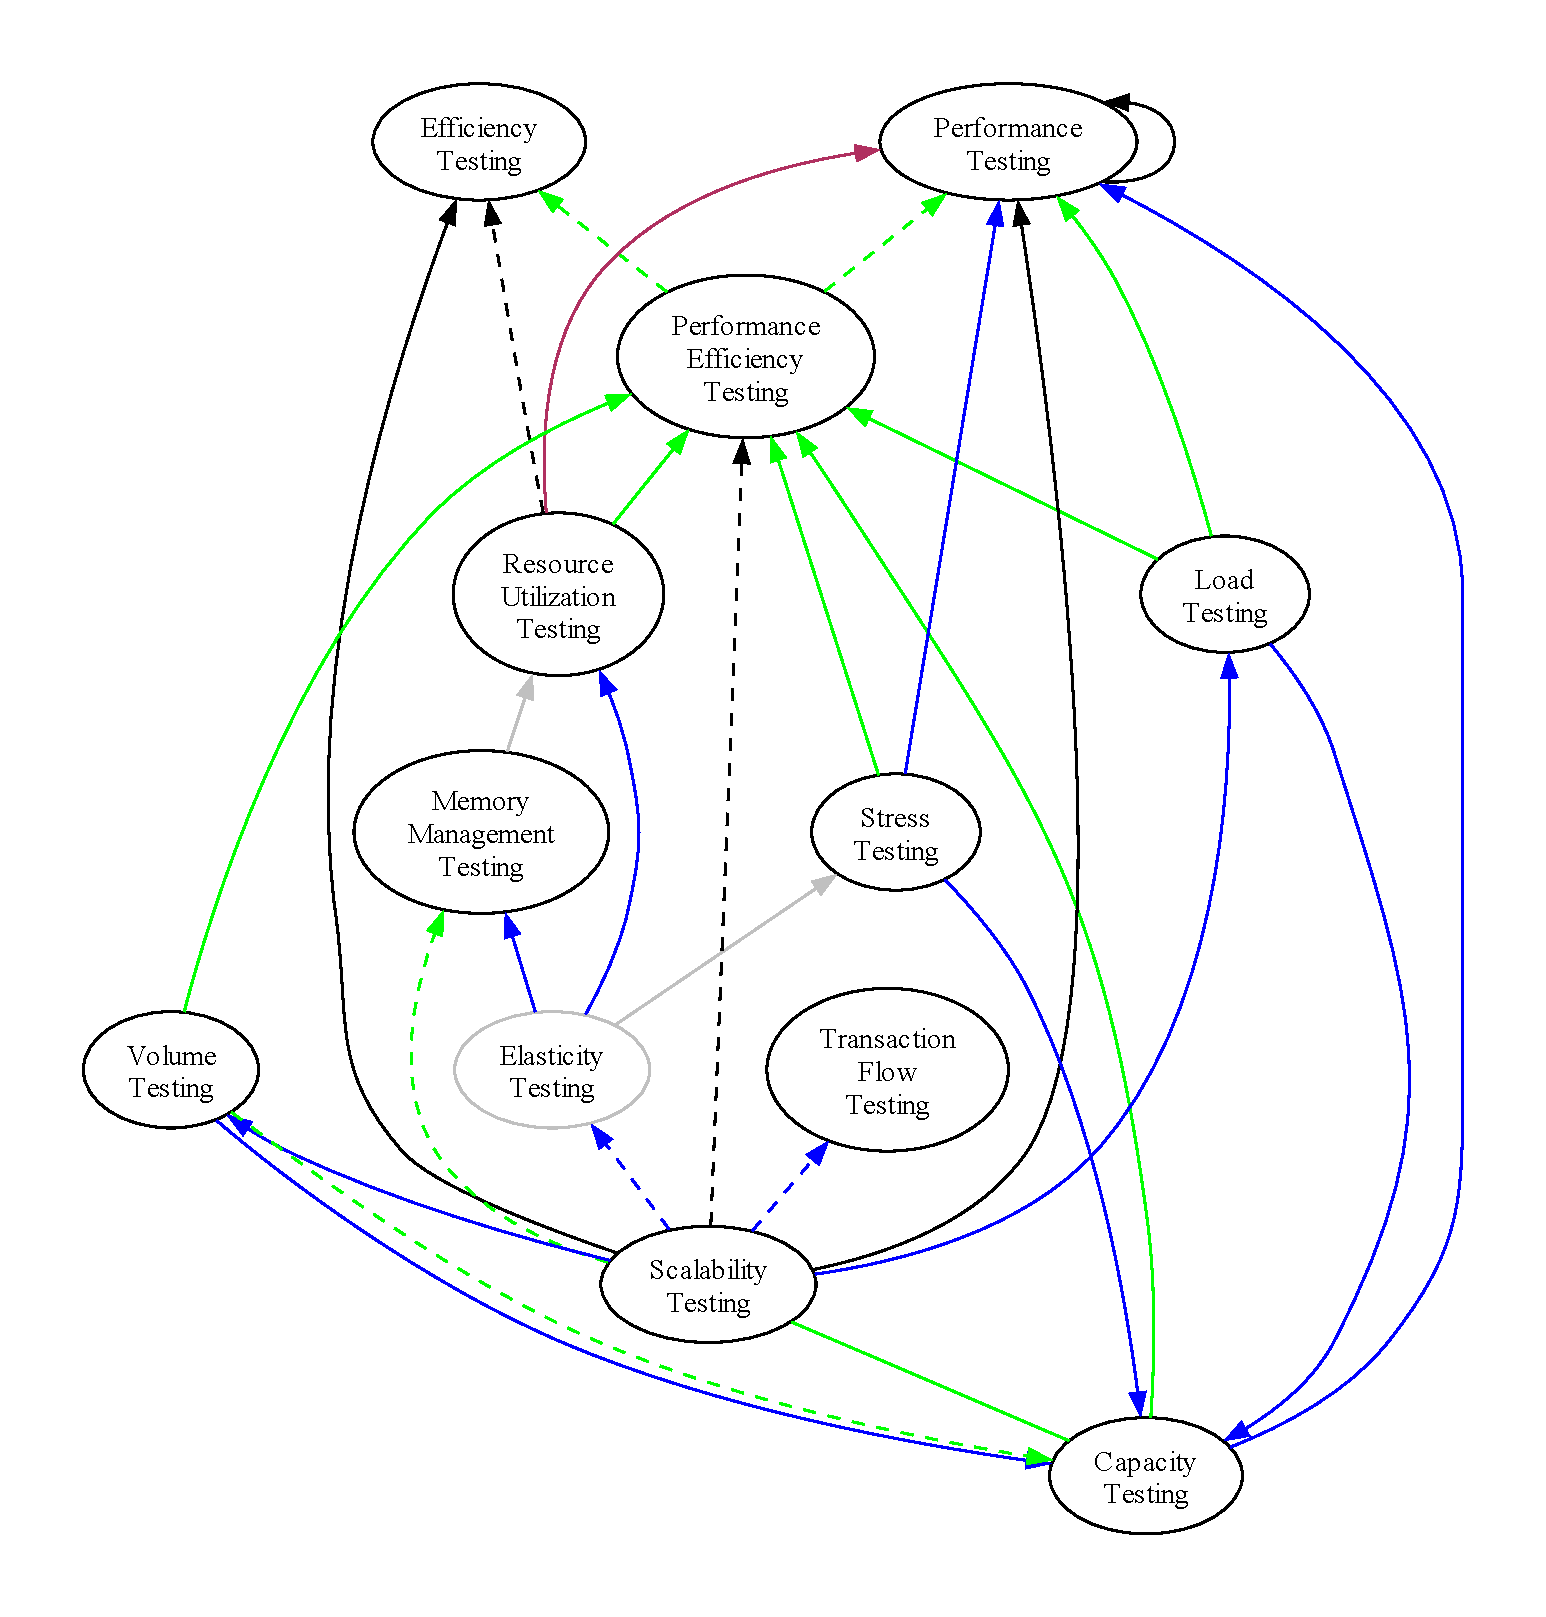
\includegraphics[width=\linewidth]{assets/graphs/scalabilityGraph.pdf}
            \caption{Graph of current relations.}
            \label{fig:scal-graph-current}
        \end{subfigure}
        \begin{subfigure}[b]{.475\linewidth}
            \centering
            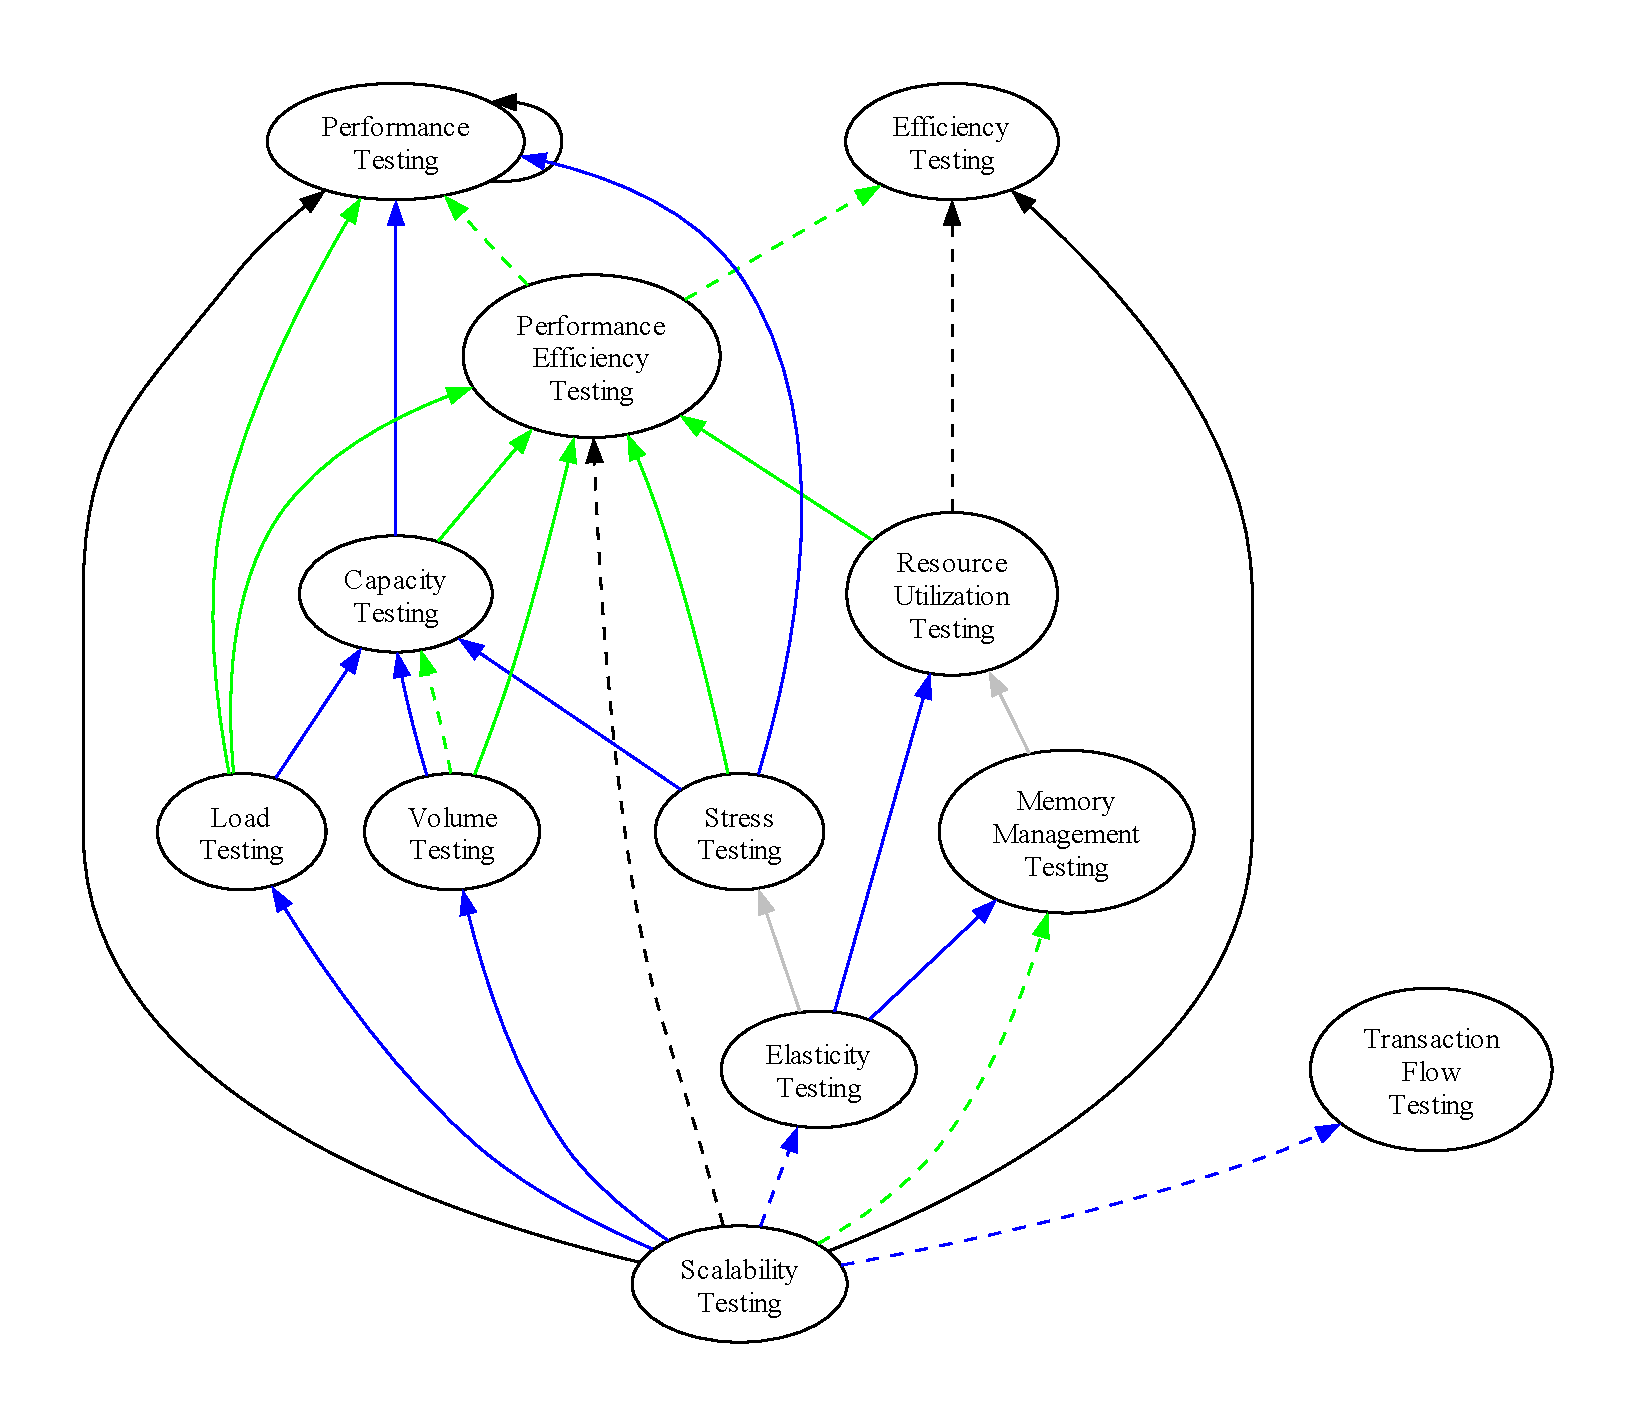
\includegraphics[width=\linewidth]{assets/graphs/scalabilityProposedGraph.pdf}
            \caption{Graph of proposed \ifnotpaper \else \\ \fi relations.}
            \label{fig:scal-graph-proposed}
        \end{subfigure}
        \caption{Graphs of relations between terms related to scalability testing.}
        \label{fig:scalGraphs}
    \end{figure}
}

\newcommand{\performanceGraph}{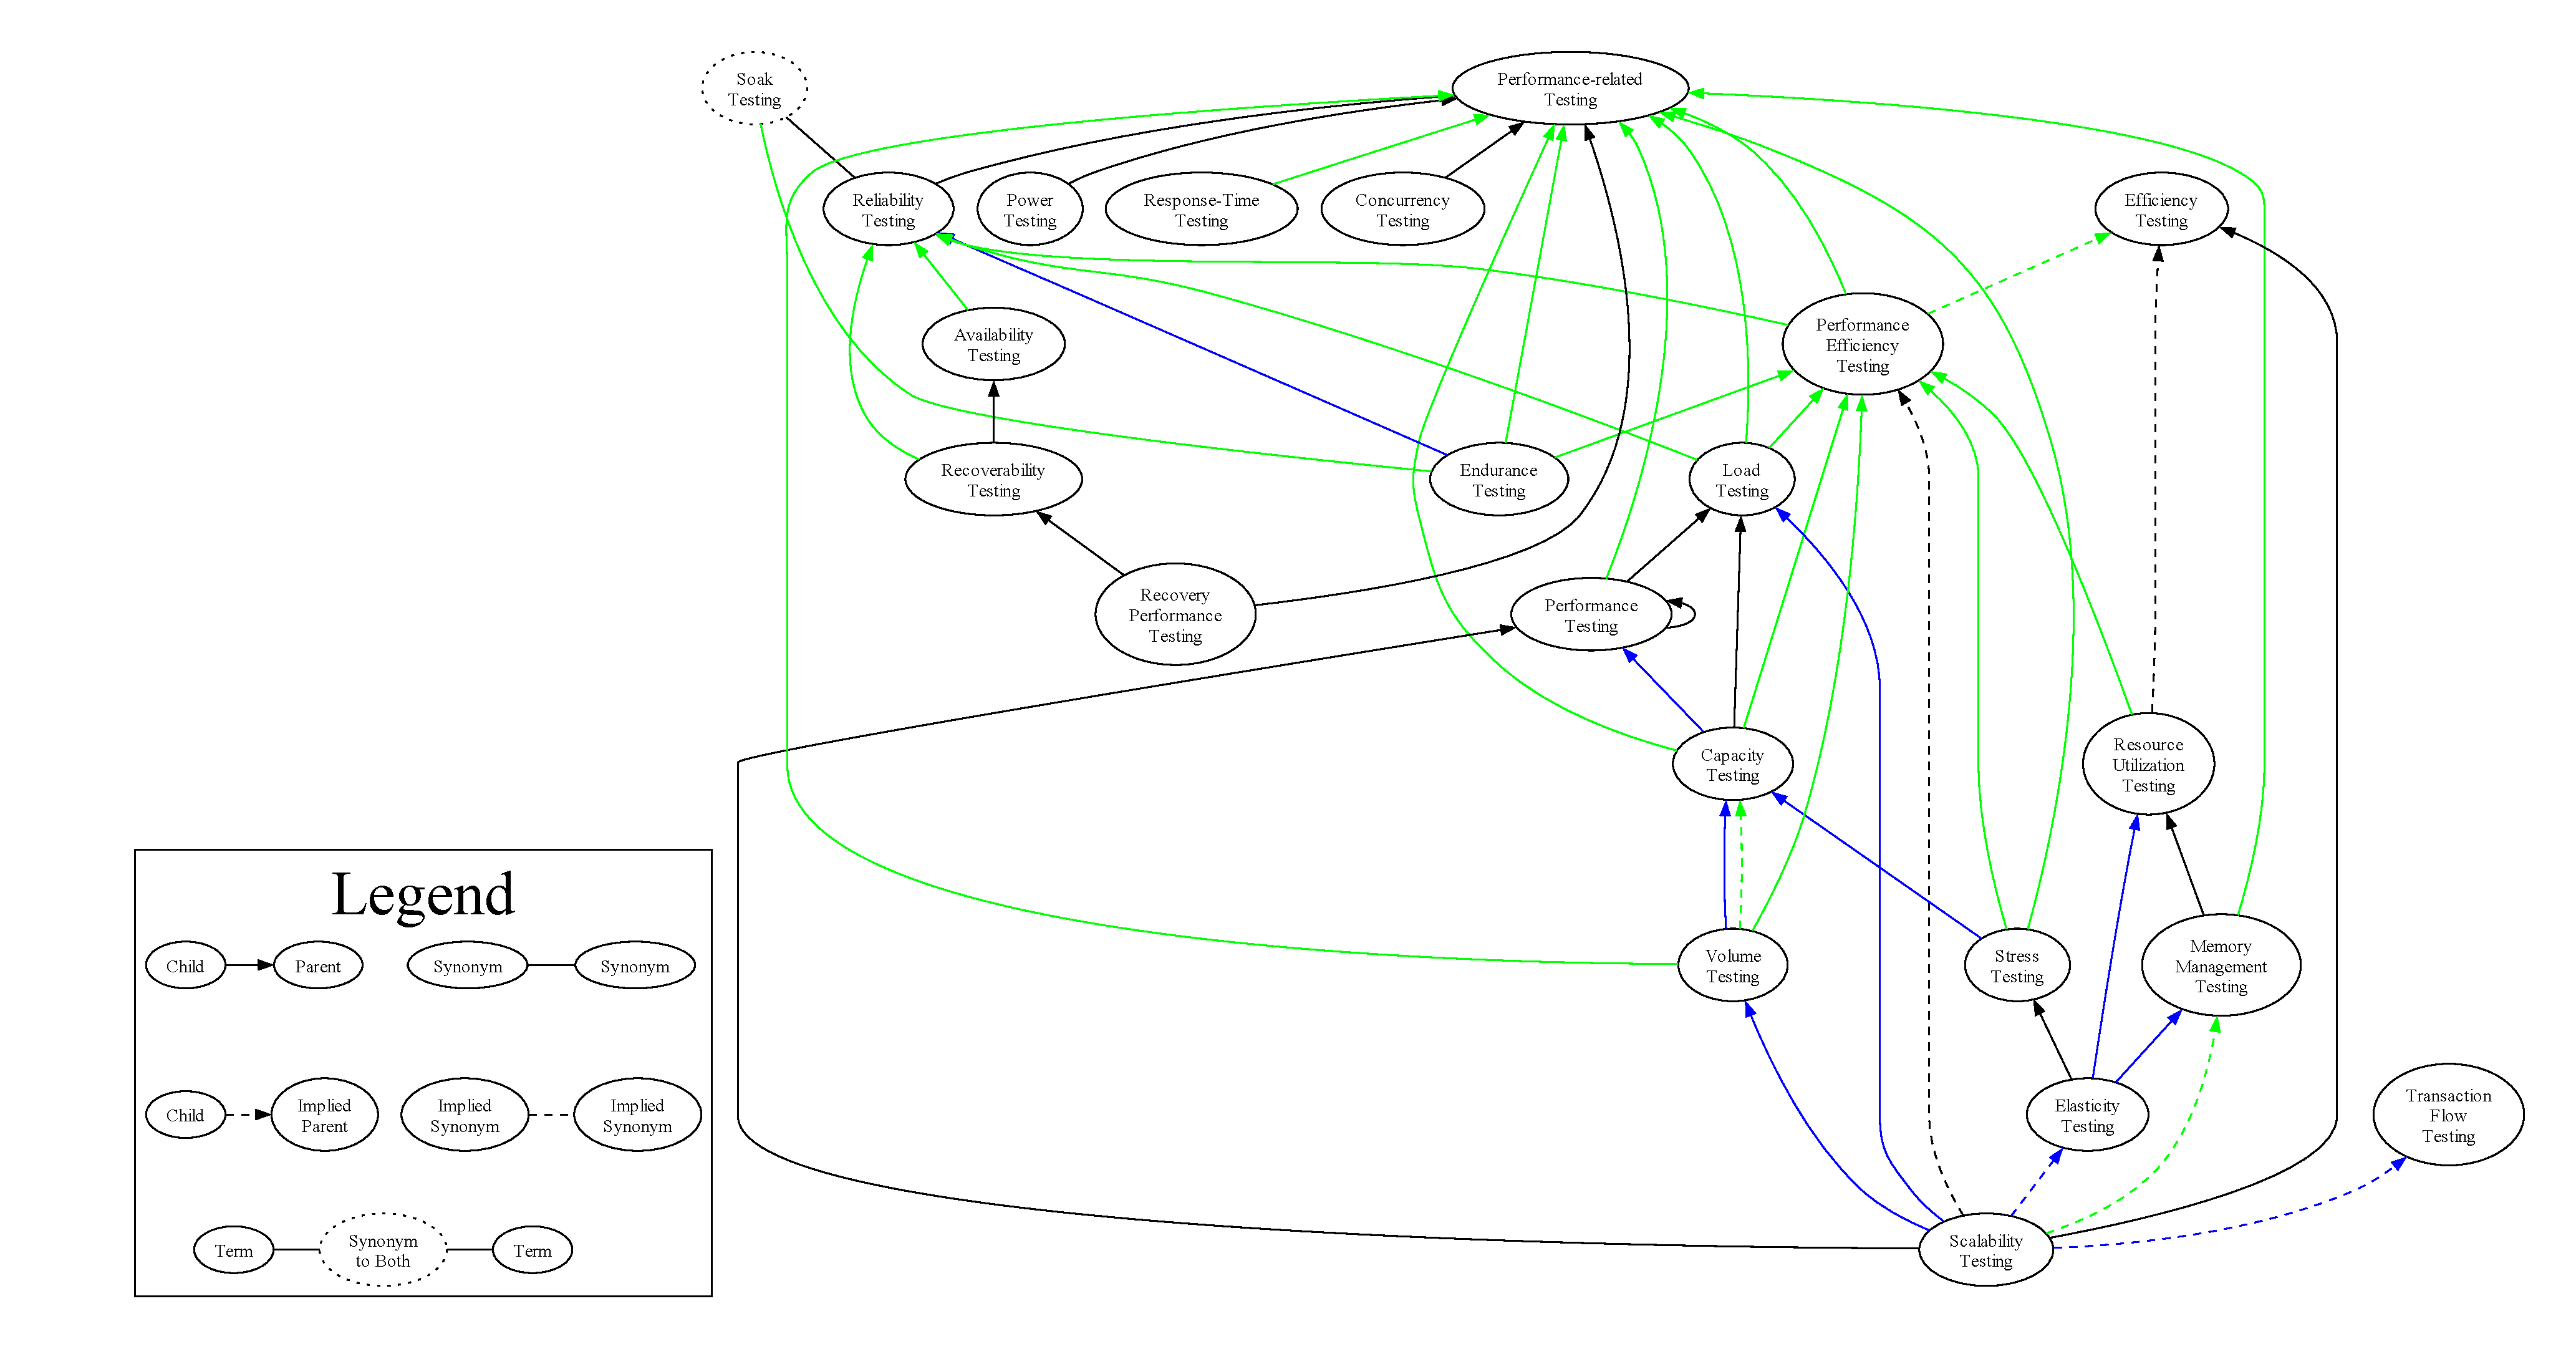
\includegraphics[width=\linewidth]{assets/graphs/performanceProposedGraph.pdf}}

%------------------------------------------------------------------------------
% Images & Figures
%------------------------------------------------------------------------------

\newcommand{\drasilLogo}{assets/images/drasil_logo.png}
\newcommand{\drasilLogoImg}{\input{assets/images/drasil_logo}}
\newcommand{\refDrasilLogoImg}{\Cref{fig:drasilLogo}}

%------------------------------------------------------------------------------
% Tables
%------------------------------------------------------------------------------

% Organization of files
\newcommand{\organizationTable}{\input{assets/tables/organization}}

\newcommand{\ieeeCatsTable}{\input{assets/tables/ieeeCats}}
\newcommand{\otherCatsTable}{\input{assets/tables/otherCats}}
\newcommand{\otherCategorizationsTable}{\input{assets/tables/otherCategorizations}}

\newcommand{\sntxFlawsTable}{\input{assets/tables/sntxFlaws}}
\newcommand{\smntcFlawsTable}{\input{assets/tables/smntcFlaws}}

\newcommand{\testReqsTable}{\input{assets/tables/testReqs}}


% Enable links within the document
\usepackage{hyperref}
\hypersetup{
    linkcolor=red,
    urlcolor=red,
    breaklinks=true,
    pdftitle={\thesisTitle{}},
}
\urlstyle{rm} % Make URL styled fonts match hyperref's hrefs
\usepackage[capitalize]{cleveref} % Fixes capitalization of internal references

% General Utility Functions
\def\sWidth{3.4cm}
\def\tWidth{0.7cm}
% Extra functionality for command parsing
\usepackage{xparse}

\newif\ifnotpaper

%------------------------------------------------------------------------------
% Reused in seminar slides
%------------------------------------------------------------------------------

\def\rqatext{What testing approaches do the literature describe?}
\def\rqbtext{Are these descriptions consistent?}
\def\rqctext{Can we systematically resolve any of these inconsistencies?}

\def\expBasedCatMain{\citeauthor{IEEE2022} categorize experience-based testing
    as both a test design technique and a test practice on the same
    page---twice \citeyearpar[Fig.~2, p.~34]{IEEE2022}!}

\NewDocumentCommand{\perfAsFamily}{s}{%
    \IfBooleanTF#1{\citealp}{\citep}[p.~1187]{Moghadam2019}\footnote{
        The original source describes ``performance testing \dots\ as a family
        of performance-related testing techniques'', but it makes more sense to
        consider ``performance-related testing'' as the ``family'' with
        ``performance testing'' being one of the variabilities
        (see \Cref{perf-test-rec}).}%
}

\def\supersAck{Drs.~Spencer Smith and Jacques Carette have been great
    supervisors in the past and have, both then and now, provided me
    with valuable guidance and feedback}

%------------------------------------------------------------------------------
% Spacing Options
%------------------------------------------------------------------------------

\newcommand{\thesisForceSingleSpacing}{\singlespacing}
\newcommand{\thesisForceDoubleSpacing}{\doublespacing}

%------------------------------------------------------------------------------
% Portable HREFs
%------------------------------------------------------------------------------

% Common variant
\newcommand{\porthref}[2]{\href{#2}{#1}\printOnlyFootnote{\url{#2}}}

% Custom URLs
\newcommand{\porthreft}[3]{\href{#3}{#1}\printOnlyFootnote{\href{#3}{#2}}}
% Inside of some environments, footnote marks aren't registered properly, so we
% need to manually write the "text" part
\newcommand{\porthreftm}[2]{\href{#2}{#1\printOnlyFootnoteMark}}

\newcommand{\formatPaper}[2]{%
    \ifnotpaper
        #1{#2}%
    \else
        \underline{#2}%
    \fi
}

\def\refHelper{\ifnotpaper\else Reference \fi}
\newcommand\multiAuthHelper[1]{\ifnotpaper #1\else #1s\fi}

\newcommand\discrepref[1]{%
    \ifnotpaper
        \labelcref{#1-discrep}%
    \else
        \Cref{#1-discrep}%
    \fi}

\newcommand\ifblind[2]{\IfEndWith*{\jobname}{_blind}{#1}{#2}}

% For `TblrNote`s in the middle of a cell (i.e., with following content)
% From https://topanswers.xyz/tex?q=4758
\ExplSyntaxOn
\NewDocumentCommand \MidTblrNote { m }
{{
            \cs_if_exist:NT \hypersetup { \ExpTblrTemplate { note-border }{ default } }
            {
                \__tblr_hyper_link:nn {#1}
                { \textsuperscript { \UseTblrFont { note-tag } #1 } }
            }
        }}
\ExplSyntaxOff

%------------------------------------------------------------------------------
% Generic "chunks" that get reused
%------------------------------------------------------------------------------

\DeclareDocumentCommand\seeSrcCode{ m m m g }{%
    (see the \href
    {https://github.com/samm82/TestGen-Thesis/blob/#1/scripts/#2.py\#L#3%
        \IfNoValueF {#4} {-L#4}}
    {relevant source code})%
}

\newcommand{\accelTolTest}{astronauts \citep[p.~11]{MorgunEtAl1999}, aviators
    \citep[pp.~27,~42]{HoweAndJohnson1995}, or catalysts
    \citep[p.~1463]{LiuEtAl2023}}

\def\recFigs{\Cref{fig:recoveryGraphs,fig:scalGraphs,fig:perf-graph}}

% Define common footnotes about IEEE testing terms for reuse
\newcommand{\distinctIEEE}[1]{distinct from the notion of ``test #1'' described
    in \Cref{tab:ieeeTestTerms}.}
\newcommand{\notDefDistinctIEEE}[1]{\footnote{Not formally defined, but
        \distinctIEEE{#1}}}
\newcommand{\gerrardDistinctIEEE}[1]{\footnote{``Each type of test addresses a
        different risk area'' \citep[p.~12]{Gerrard2000a}, which is
        \distinctIEEE{#1}}}

% Examples of discrepancies
\NewDocumentCommand\tourDiscrep{s}{%
    \IfBooleanTF#1{t}{T}he structure of tours can be defined as either quite
    general \citep[p.~34]{IEEE2022} or ``organized around a special focus''
    \citepISTQB{}\IfBooleanTF#1{}{.}}
\def\alphaDiscrep{Alpha testing is performed by ``users within the organization
    developing the software'' \citep[p.~17]{IEEE2017}, ``a small, selected
    group of potential users'' \citep[p.~5-8]{SWEBOK2024}, or ``roles outside
    the development organization'' conducted ``in the developer's test
    environment'' \citepISTQB{}.}
\def\loadDiscrep{Load testing is performed with loads ``between anticipated
    conditions of low, typical, and peak usage'' \citep[p.~5]{IEEE2022} or
    loads that are as large as possible \citep[p.~86]{Patton2006}.}

\def\suggSrcs{\href
    {https://github.com/samm82/TestGen-Thesis/issues/14\#issuecomment-1839922715}
    {suggested by Dr.~Carette}}

% Used in parSyns tables
\def\ftrnote{Fault tolerance testing may also be a sub-approach of
    reliability testing \ifnotpaper
        \citetext{\citealp[p.~375]{IEEE2017}; \citealp[p.~7-10]{SWEBOK2024}}%
    \else \cite[p.~375]{IEEE2017}, \cite[p.~7-10]{SWEBOK2024}%
    \fi, which is distinct from robustness testing \citep[p.~53]{Firesmith2015}.}
\def\specfn{See \Cref{spec-func-test}.}
\def\ucstn{See \discrepref{use-case-scenario}.}

%------------------------------------------------------------------------------
% For populating values from files
%------------------------------------------------------------------------------

\ExplSyntaxOn
\ior_new:N \g_hringriin_file_stream

\NewDocumentCommand{\ReadFile}{mm}
{
    \hringriin_read_file:nn { #1 } { #2 }
    \cs_new:Npn #1 ##1
    {
        \str_if_eq:nnTF { ##1 } { * }
        { \seq_count:c { g_hringriin_file_ \cs_to_str:N #1 _seq } }
        { \seq_item:cn { g_hringriin_file_ \cs_to_str:N #1 _seq } { ##1 } }
    }
}

\cs_new_protected:Nn \hringriin_read_file:nn
{
    \ior_open:Nn \g_hringriin_file_stream { #2 }
    \seq_gclear_new:c { g_hringriin_file_ \cs_to_str:N #1 _seq }
    \ior_map_inline:Nn \g_hringriin_file_stream
    {
        \seq_gput_right:cx
        { g_hringriin_file_ \cs_to_str:N #1 _seq }
        { \tl_trim_spaces:n { ##1 } }
    }
    \ior_close:N \g_hringriin_file_stream
}

\ExplSyntaxOff

% Define/read values for Undefined Terms methodology for reuse and calculation!
\ReadFile{\undefTermCounts}{assets/misc/undefTermCounts}

\newcount\TotalBefore
\newcount\UndefBefore
\newcount\TotalAfter
\newcount\UndefAfter

\TotalBefore=\undefTermCounts{1}
\UndefBefore=\undefTermCounts{2}
\TotalAfter=\undefTermCounts{3}
\UndefAfter=\undefTermCounts{4}

\def\approachCount{\undefTermCounts{3}}

\ReadFile{\qualityCounts}{build/qualityCount}
\def\qualityCount{\qualityCounts{1}}

\ReadFile{\parSynCounts}{build/parSynCounts}
\def\parSynCount{\parSynCounts{1}}
\def\selfCycleCount{\parSynCounts{2}}

\ReadFile{\stdSources}{build/stdSources}
\ReadFile{\metaSources}{build/metaSources}
\ReadFile{\textSources}{build/textSources}
\ReadFile{\paperSources}{build/paperSources}

\def\srcCount{\the\numexpr\stdSources{3} + \metaSources{3} + \textSources{3} + \paperSources{3}}

\ReadFile{\stdSmntcDiscBrkdwn}{build/stdSmntcDiscBrkdwn}
\ReadFile{\metaSmntcDiscBrkdwn}{build/metaSmntcDiscBrkdwn}
\ReadFile{\textSmntcDiscBrkdwn}{build/textSmntcDiscBrkdwn}
\ReadFile{\paperSmntcDiscBrkdwn}{build/paperSmntcDiscBrkdwn}
\ReadFile{\totalSmntcDiscBrkdwn}{build/totalSmntcDiscBrkdwn}

\ReadFile{\stdSntxDiscBrkdwn}{build/stdSntxDiscBrkdwn}
\ReadFile{\metaSntxDiscBrkdwn}{build/metaSntxDiscBrkdwn}
\ReadFile{\textSntxDiscBrkdwn}{build/textSntxDiscBrkdwn}
\ReadFile{\paperSntxDiscBrkdwn}{build/paperSntxDiscBrkdwn}
\ReadFile{\totalSntxDiscBrkdwn}{build/totalSntxDiscBrkdwn}

\def\stds{\nameref{stds}}
\def\metas{\nameref{metas}}
\def\texts{\nameref{texts}}
\def\papers{\nameref{papers}}
\def\papersTbl{\hyperref[papers]{Papers and Others}}

\def\srcCat{\hyperref[sources]{Source Tier}}
\def\reduns{\ifnotpaper\nameref{redun}\else Redundancies\footnote{Section omitted for brevity.}\fi}

\def\totalDiscreps{\totalSmntcDiscBrkdwn{13}}

\def\cats{\hyperref[cats]{Categories}}
\def\syns{\hyperref[syns]{Synonyms}}
\def\pars{\hyperref[pars]{Parents}}
\def\defs{\hyperref[defs]{Definitions}}
\def\terms{\hyperref[terms]{Terminology}}
\def\cites{\hyperref[cites]{Citations}}

%------------------------------------------------------------------------------
% TODOs
%------------------------------------------------------------------------------

% Generic Inlined TODOs
\newcommand{\intodo}[1]{\todo[inline]{#1}}

% Unimportant TODOs for "later" (i.e., finishing touches or changes immediately before submission)
\newcommand{\latertodo}[1]{\todo[backgroundcolor=Cyan]{\textit{Later}: #1}}

% "Important" TODOs
\newcommand{\imptodo}[1]{\todo[inline,backgroundcolor=Red]{\textbf{Important}: #1}}

% "Easy" TODOs
\newcommand{\easytodo}[1]{\todo[inline,backgroundcolor=SeaGreen]{\textit{Easy}: #1}}
\newcommand{\eztodo}[1]{\easytodo{#1}}

% "Tedious" TODOs
\newcommand{\tedioustodo}[1]{\todo[inline,backgroundcolor=PineGreen]{\textit{Needs time}: #1}}

% "Question" TODO Notes
\newcounter{todonoteQuestionsCtr}
\newcommand{\questiontodo}[1]{\stepcounter{todonoteQuestionsCtr}\todo[backgroundcolor=Lavender]{\textbf{Q \#\thetodonoteQuestionsCtr{}}: #1}}
\newcommand{\qtodo}[1]{\questiontodo{#1}}

% Specific categories of TODOs
\def\ptq{\todo{Present tense?}}

%------------------------------------------------------------------------------
% Citations
%------------------------------------------------------------------------------

\newcommand{\exhInfCite}{(\citealp[p.~5-5]{SWEBOK2024}; \citealp[p.~4]{IEEE2022};
    \citealp[p.~421]{vanVliet2000}; \citealp[pp.~439, 461]{PetersAndPedrycz2000})}

%------------------------------------------------------------------------------
% Link to Drasil issue
%------------------------------------------------------------------------------

\newcommand{\issueref}[1]{\href{https://github.com/JacquesCarette/Drasil/issues/#1}{\##1}}
\newcommand{\pullref}[1]{\href{https://github.com/JacquesCarette/Drasil/pull/#1}{\##1}}
\newcommand{\thesisissuerefhelper}[1]{\href{https://github.com/samm82/TestGen-Thesis/issues/#1}{\##1}}

\ExplSyntaxOn

% Based on output from ChatGPT
\NewDocumentCommand{\mapthesisissueref}{m}
{
    % Clear temporary sequences to store transformed items
    \seq_clear:N \l_tmpa_seq
    \seq_clear:N \l_tmpb_seq

    \seq_set_split:Nnn \l_tmpa_seq { , } { #1 } % Split the input by commas
    \seq_map_inline:Nn \l_tmpa_seq
    {
        \seq_put_right:Nn \l_tmpb_seq {\thesisissuerefhelper{##1}}
    }
    \seq_use:Nnnn \l_tmpb_seq { ~and~ } { ,~ } { ,~and~ }
}

\ExplSyntaxOff

\newcommand{\thesisissueref}[1]{\todo[backgroundcolor=lightgray]{See \mapthesisissueref{#1}}}


\usepackage{cite}
\newcommand{\citetISTQB}{\cite{ISTQB}}
\newcommand{\citepISTQB}{\cite{ISTQB}}
\newcommand{\citealpISTQB}{\cite{ISTQB}}
\newcommand{\citeauthor}{\cite}
\newcommand{\citeauthorpar}{\cite}
\newcommand{\citeyearpar}{\cite}
\newcommand{\citeyear}{\cite}
\newcommand{\citet}{\cite}
\newcommand{\citep}{\cite}
\newcommand{\citealp}{\cite}
\newcommand{\citetext}[1]{[#1]}

\usepackage{algorithmic}
\usepackage{textcomp}

\usepackage[disable]{todonotes}

\usepackage{xstring}

\newenvironment{paperTable}{
    \begingroup
    \renewcommand*{\thefootnote}{\alph{footnote}}
    \begin{table*}[t!]
        }{
    \end{table*}
    \endgroup
}

\newenvironment{paperFigure}{
    \begin{figure*}[t!]
        }{
    \end{figure*}
}

\newcommand{\acf}[1]{(\uppercase{#1})}
\newcommand{\acs}[1]{\uppercase{#1}}

\def\BibTeX{{\rm B\kern-.05em{\sc i\kern-.025em b}\kern-.08em
    T\kern-.1667em\lower.7ex\hbox{E}\kern-.125emX}}
\begin{document}

\title{Putting Software Testing Terminology to the Test\\
    % Sub-titles should not be used!
    \thanks{Funding for this work was provided by the Ontario Graduate
        Scholarship and McMaster University.}
}

% % Double-blind
% \author{Author details suppressed}

% Current version
\author{\IEEEauthorblockN{Samuel J. Crawford\IEEEauthorrefmark{1},
        Spencer Smith\IEEEauthorrefmark{1}, Jacques Carette\IEEEauthorrefmark{1}}
    \IEEEauthorblockA{\IEEEauthorrefmark{1}Department of Computing and Software \\
        McMaster University\\
        Hamilton, Canada \\
        \{crawfs1, smiths, carette\}@mcmaster.ca}}

% % Previous version (weird formatting)
% \newcommand{\deptCAS}[1]{
%     \IEEEauthorblockA{\textit{Department of Computing and Software} \\
%         \textit{McMaster University}\\
%         Hamilton, Canada \\
%         #1@mcmaster.ca}}

% \author{\IEEEauthorblockN{Samuel~J.~Crawford}
%     \deptCAS{crawfs1}
%     \and
%     \IEEEauthorblockN{Spencer~Smith}
%     \deptCAS{smiths}
%     \and
%     \IEEEauthorblockN{Jacques~Carette}
%     \deptCAS{carette}
% }

\maketitle

\begin{abstract}
    Testing is a pervasive software development activity that is often
    complicated and expensive (if not simply overlooked).  This is in
    part due to an unstable knowledge base: there is no standard, consistent,
    and ``complete'' taxonomy for software testing, inhibiting precise
    communication.
    Discrepancies and ambiguities are widespread throughout the literature, and
    sometimes exist between different parts of the same document!
    % Therefore, automating the software testing process is an area of interest,
    % and understanding the underlying domain is an important prerequisite.
    We systematically investigate the current state of software terminology.
    We 1) identify established standards
    and prominent testing resources,
    2) capture relevant testing terms
    from these sources, along with their definitions and relationships (both
    explicit and implied), and
    3) build graphs to visualize and analyze
    this data. Over five hundred test approaches were
    uncovered, as well as
    some methods for describing ``implied'' test approaches. We also build
    a tool to generate graphs of the relations between test
    approaches and track ambiguities captured by this tool and
    manually through the research process. Our results show ten terms are
    given as synonyms to two (or more) disjoint test approaches and fourteen
    pairs of test approaches may be synonyms and/or have a child-parent
    relationship. There is also confusion surrounding functional, recovery,
    scalability, and performance testing, along with over fifty more
    ``minor'' discrepancies. Overall, there is a need for testing terminology
    to be standardized to make the discussion, analysis, and implementation of
    various test approaches more coherent. We
    provide some preliminary advice on how to accomplish this.
\end{abstract}

\begin{IEEEkeywords}
    Software testing, terminology, taxonomy, literature review, test approaches
\end{IEEEkeywords}

\section{Background}

% TODO: tighten up, add sources

Testing software is complicated, expensive, and often overlooked.
Improving the productivity of testing and testing research requires a standard
language for communication. Unfortunately, a search
for a systematic, rigorous, and ``complete'' taxonomy for software testing
revealed that the existing ones are inadequate:

\begin{itemize}
    \item Tebes et al. \cite{TebesEtAl2020a} focus on \emph{parts} of the
          testing process (e.g., test goal, testable entity),
    \item Souza et al. \cite{SouzaEtAl2017} prioritize organizing testing
          approaches over defining them, and
    \item Unterkalmsteiner et al. \cite{UnterkalmsteinerEtAl2014} provide a
          foundation for classification but not how it applies to software
          testing terminology.
\end{itemize}

Thus we set about closing this gap. We first define the scope of what kinds of
``software testing'' are of interest (\Cref{scope}) and examine the existing
literature (\Cref{method}). This reinforces the need for a proper taxonomy!
Despite the amount of well understood and organized knowledge (\Cref{observ}),
there are still many discrepancies and ambiguities in the literature, either
within the same source or between various sources (\Cref{discrep}). We provide
some potential solutions covering some of these discrepancies (\Cref{recs}).

\section{Scope}
\label{scope}

This project is focused on the generation of test cases for code, so only
the ``testing'' component of \acf{vnv} is considered (see \thesisissueref{22}).
For example, design reviews (see \citealp[p.~132]{IEEE2017}) and
documentation reviews (see \citealp[p.~144]{IEEE2017}) are out of scope,
since they focus on the \acs{vnv} of the design and documentation of the code,
respectively, and not on the code itself. Likewise, ergonomics testing
and proximity-based testing (see \citealpISTQB{}) are out of scope since
they are for testing hardware systems, as is \acf{emsec} testing
(\citealp{ISO2021}; \citealp[p.~95]{ZhouEtAl2012}), which deals with the
``security risk'' of ``information leakage via electromagnetic emanation''
\citep[p.~95]{ZhouEtAl2012}. Security audits that focus on ``an organization's
\dots\ processes and infrastructure'' \citepISTQB{}, are also out of scope,
but security audits that ``aim to ensure that all of the products installed on
a site are secure when checked against the known vulnerabilities for those
products'' \citep[p.~28]{Gerrard2000b} are not. While \acf{oat}
can be used when testing software \citep{Mandl1985}, it can also be used for
hardware \citep[pp.~471-472]{Valcheva2013}, such as ``processors \dots\ made
from pre-built and pre-tested hardware components'' (p.~471). A subset of
\acs{oat} called ``\acf{toat}'' is used for ``experimental design problems in
manufacturing'' \citep[p.~1573]{YuEtAl2011} or ``product and manufacturing
process design'' \cite[p.~44]{Tsui2007} and is thus out of scope.

This sometimes leads to making wider decisions on whether a whole category of
testing is in scope. For example, while all the examples of domain-specific
testing given by \citet[p.~26]{Firesmith2015} are focused on hardware, this
might not be representative of all types (e.g., ML model testing seems
domain-specific).
\ifnotpaper
    Conversely, the examples of environmental tolerance testing
    (p.~56) do not seem to apply to software. For example, radiation tolerance
    testing seems to focus on hardware, such as motors \citep{MukhinEtAl2022},
    robots \citep{ZhangEtAl2020}, or ``nanolayered carbide and nitride materials''
    \citep[p.~1]{TunesEtAl2022}. Acceleration tolerance testing seems to focus on
    \accelTolTest{} and acoustic tolerance testing on rats \citep{HolleyEtAl1996},
    which are even less related! Since these all seem to focus on
    environment-specific factors that would not impact the code, this category of
    testing is also out of scope.

    It is also interesting to note that different test approaches seem to be more
    specific to certain domains. For example, the terms ``software qualification
    testing'' and ``system qualification testing'' show up throughout
    \citep{SPICE2022}, which was written for the automotive industry, and the more
    general idea of ``qualification testing'' seems to refer to the process of
    making a hardware component, such as an electronic component
    \citep{AhsanEtAl2020}, gas generator \citep{ParateEtAl2021} or photovoltaic
    device, ``into a reliable and marketable product'' \citep[p.~1]{SuhirEtAl2013}.
\fi

This also means that only some aspects of some testing approaches are relevant.
This mainly manifests as a testing approach that can verify both the \acs{vnv}
itself and the code. For example:

\begin{enumerate}
    \item \emph{Error seeding} is the ``process of intentionally adding
          known faults to those already in a computer program'',
          done to both ``monitor[] the rate of detection and removal'',
          which is a part of \acs{vnv} of the \acs{vnv} itself, ``and
          estimat[e] the number of faults remaining''
          \citep[p.~165]{IEEE2017}, which helps verify the actual code.
    \item \emph{Fault injection testing}, where ``faults are artificially
          introduced into the \acs{sut}'', can be used to evaluate the
          effectiveness of a test suite \citep[p.~5-18]{SWEBOK2024},
          which is a part of \acs{vnv} of the \acs{vnv} itself, or ``to test
          the robustness of the system in the event of internal and
          external failures'' \citep[p.~42]{IEEE2022}, which helps verify
          the actual code.
    \item ``\emph{Mutation [t]esting} was originally conceived as a
          technique to evaluate test suites in which a mutant is a slightly
          modified version of the \acs{sut}'' \citep[p.~5-15]{SWEBOK2024},
          which is in the realm of \acs{vnv} of the \acs{vnv} itself.
          However, it ``can also be categorized as a structure-based
          technique'' and can be used to assist fuzz and metamorphic testing
          \citep[p.~5-15]{SWEBOK2024}.
    \item Even though \emph{reliability testing} and \emph{maintainability
              testing} can start \emph{without} code by ``measur[ing]
          structural attributes of representations of the software''
          \citep[p.~18]{FentonAndPfleeger1997}, only reliability and
          maintainability testing done \emph{on} code is in scope.
          \ifnotpaper
    \item Since control systems often have a software \emph{and} hardware
          component \citep{ISO2015, PreußeEtAl2012,ForsythEtAl2004},
          only the software component is in scope. In some cases, it is
          unclear whether the ``loops''\footnote{Humorously, the testing of
              loops in chemical systems \citep{Dominguez-PumarEtAl2020} and
              copper loops \citep{Goralski1999} are out of scope.} being
          tested are implemented by software or hardware, such as those in
          wide-area damping controllers \citep{PierreEtAl2017, TrudnowskiEtAl2017}.
          \begin{itemize}
              \item A related note: ``path coverage'' or ``path testing''
                    seems to be able to refer to either paths through code
                    (as a subset of control-flow testing)
                    \citep[p.~5-13]{SWEBOK2024} or through a model, such as
                    a finite-state machine (as a subset of model-based
                    testing) \citep[p.~184]{DoğanEtAl2014}.
          \end{itemize}
          \fi
\end{enumerate}

\ifnotpaper
    Specific programming languages are sometimes used to define ``kinds'' of
    testing. These will not be included (see \thesisissueref{63}); if the reliance
    on a specific programming language is intentional, then this really implies an
    underlying test approach that may be generalized to other languages. Some
    examples:

    \begin{itemize}
        \item ``They implemented an approach \dots\ for JavaScript testing
              (referred to as Randomized)'' \citep[p.~192]{DoğanEtAl2014} -
              this really refers to random testing used within JavaScript
        \item ``SQL statement coverage'' is really just statement coverage
              used specifically for SQL statements \citep[Tab.~13]{DoğanEtAl2014}
              \todo{OG Alalfi et al., 2010}
        \item ``Faults specific to PHP'' is just a subcategory of fault-based
              testing, since ``execution failures \dots\ caused by missing an
              included file, wrong MySQL quer[ies] and uncaught exceptions''
              are not exclusive to PHP \citep[Tab.~27]{DoğanEtAl2014}
              \todo{OG Artzi et al., 2008}
        \item While ``HTML testing'' is listed or implied by
              \citeauthor{Gerrard2000a} (\citeyear[Tab.~2]{Gerrard2000a};
              \citeyear[Tab.~1, p.~3]{Gerrard2000b}) and
              \citet[p.~220]{Patton2006}, it seems to be a combination of syntax
              testing, functionality testing, hyperlink testing/link checking,
              cross-browser compatibility testing, performance testing, and
              content checking \citep[p.~3]{Gerrard2000b}
    \end{itemize}
\fi

\subsection{Static Testing}
\label{static-test}
Sometimes, the term ``testing'' excludes static testing
(\citealp[p.~222]{AmmannAndOffutt2017}; \citealp[p.~13]{Firesmith2015});
restricting it to ``dynamic validation'' \citep[p.~5-1]{SWEBOK2024} or
``dynamic verification'' ``in which a system or component is
executed'' \citep[p.~427]{IEEE2017}. Since ``terminology is not uniform
among different communities, and some use the term \emph{testing} to refer to
static techniques\notDefDistinctIEEE{technique} as well''
\citep[p.~5-2]{SWEBOK2024} (such as \citep[pp.~8-9]{Gerrard2000a} and even
\citep[p.~440]{IEEE2017}!), the scope of ``testing'' for the purpose of this
project originally included both ``static testing'' and ``dynamic testing'', as
done by \citet[p.~17]{IEEE2022}. However, static testing tends to be less
systematic/consistent and often requires human intervention, which makes it
less relevant to this project's end goal: to generate test cases automatically.
However, understanding the breadth of testing approaches provides a more
complete picture of how software can be tested, how the various approaches are
related to one another, and potentially how even parts of these ``out-of-scope''
approaches may be generated in the future! These ``out-of-scope'' approaches
will be identified more systematically, but gathering information about them is
an important precursor, making them within the scope of this research, although
they will be excluded at a later phase. Even some dynamic methods, such as
demonstrations and dynamic analysis, which fall under the realm of ``evaluation''
as opposed to ``testing'' \citep[p.~13]{Firesmith2015} may be out of scope, due
to their reliance on human intervention.
\section{Methodology}
\label{method}

\subsection{Sources}
\label{sources}
As there is no single authoritative source on software testing terminology,
we need to look at many. Unfortunately, this brings to light a variety of
discrepancies. Starting from some set of sources, we then use
``snowballing'' % needs a reference!
to gather further sources\seeParAlways{undef-terms}. Groups of sources with
information that shows up in a relevant graph are given a unique colour to
better visualize them; see \Cref{fig:recovery-graph-current,%
      fig:recovery-graph-proposed,fig:scal-graph-current,%
      fig:scal-graph-proposed,fig:perf-graph}.

\begin{enumerate}
      \setcounter{enumi}{-1}
      \item Trusted textbooks
            \citep{Patton2006, PetersAndPedrycz2000, vanVliet2000}
            \begin{itemize}
                  \item Ad hoc and arbitrary; not systematic
                        % \item Colored \textcolor{Maroon}{maroon},
            \end{itemize}
      \item Established standards, such as IEEE, ISO/IEC, and the \acf{swebok}
            \begin{itemize}
                  \item Standards organizations \citep{IEEE2022, IEEE2017,
                              IEEE2013, ISO_IEC2023b, IEEE2012, ISO_IEC2023a,
                              IEEE2021, ISO_IEC2018, ISO2021, ISO2015}
                        colored \textcolor{green}{green}
                  \item ``Meta-level'' commentaries or collections of
                        terminology (often based on these standards)
                        \ifnotpaper
                              (\citealp{SWEBOK2024, SWEBOK2014};
                              \citealpISTQB{}; \citealp{Firesmith2015})
                        \else
                              \cite{SWEBOK2024, SWEBOK2014, ISTQB, Firesmith2015}
                        \fi colored \textcolor{blue}{blue},
            \end{itemize}
      \item Other resources: less-formal classifications of terminology
            \ifnotpaper
                  \citep[e.g.,][]{KuļešovsEtAl2013}%
            \else
                  (such as \citep{KuļešovsEtAl2013})%
            \fi%
            , sources investigated to
            ``fill in'' missing definitions\seeSectionParAlways{undef-terms},
            and testing-related resources that emerged for unrelated reasons
            \begin{itemize}
                  \item Colored black, along with any ``surface-level''
                        analysis that followed straightforwardly.
            \end{itemize}
\end{enumerate}

\subsection{Procedure}

To track terminology used in the literature, we build a glossary of test
approaches, including the term itself, its definition, and
any synonyms or parents. Many test approaches are multi-faceted and can be
``specialized'' into others, such as \nameref{perf-test-rec}. These
``specializations'' will be referred to as ``children'' or
``sub-approaches\footnote{This nomenclature extends to other categories of
      approaches from \Cref{tab:ieeeTestTerms}, such as ``sub-type''.}''
of the multi-faceted
``parent''. Any additional notes, such as questions or sources to investigate
further, are also recorded. Approach categorizations, such as those found in
\Cref{tab:ieeeTestTerms} and some outliers (e.g., ``artifact''), are tracked
for future investigation.

All sources are analyzed in their entirety to systematically extract
terminology. (Some sources given in \Cref{undef-terms}
were only partially investigated to focus on the area of interest or since
the test approach was determined to be out-of-scope.)
Heuristics are used to guide this process, by investigating:

\begin{itemize}
      \item glossaries and lists of terms,
      \item testing-related terms (e.g., terms containing ``test(ing)'',
            \ifnotpaper ``review(s)'', ``audit(s)'', \fi
            ``validation'', or ``verification''),
      \item terms that had emerged as part of already-discovered
            testing approaches, \emph{especially} those that were ambiguous
            or prompted further discussion (e.g., terms containing
            ``performance'', ``recovery'', ``component'', ``bottom-up'',
            \ifnotpaper ``boundary'', \fi or ``configuration''), and
      \item terms that implied testing approaches%
            \ifnotpaper\footnote{
                        Since these methods for deriving test approaches only arose
                        as research progressed, some examples would have been missed
                        during the first pass(es) of resources investigated earlier
                        in the process. While reiterating over them would be ideal,
                        this may not be possible due to time constraints.
                  }\fi%
            \seeSectionParAlways{derived-tests}.
\end{itemize}

When terms have multiple definitions, either the clearest and most concise
version is kept, or they are merged to paint a more complete picture.
If any discrepancies or ambiguities
arise, they are reasonably investigated and always documented. If a
testing approach is mentioned but not defined, it is added to the
glossary to indicate it should be investigated further%
\seeSectionParAlways{undef-terms}. A similar methodology
is used for tracking software qualities, albeit in a separate
document\seeSectionParAlways{qual-test}.

During the first pass of data collection, all software-testing-focused terms
are included. Some of them are less applicable to test case automation
\ifnotpaper{(such as \Cref{static-test}, \thesisissueref{39})}\fi or too
broad (such as \Cref{attacks}\ifnotpaper{, \thesisissueref{55}}\fi), so they
will be omitted over the course of analysis.

\ifnotpaper
      During this investigation, some terms came up that seemed to be relevant to
      testing but were so vague, they didn't provide any new information. These were
      decided to be not worth tracking\seeThesisIssuePar{39}[, \thesisissueref{44},
            \thesisissueref{28}] and are listed below:

      \begin{itemize}
            \item \textbf{Evaluation:} the ``systematic determination of the extent
                  to which an entity meets its specified criteria''
                  \citep[p.~167]{IEEE2017}
            \item \textbf{Product Analysis:} the ``process of evaluating a product by
                  manual or automated means to determine if the product has certain
                  characteristics'' \citep[p.~343]{IEEE2017}
            \item \textbf{Quality Audit:} ``a structured, independent process to
                  determine if project activities comply with organizational and
                  project policies, processes, and procedures'' \citep[p.~361]{IEEE2017}
                  \todo{OG PMBOK}
            \item \textbf{Software Product Evaluation:} a ``technical operation that
                  consists of producing an assessment of one or more characteristics
                  of a software product according to a specified procedure''
                  \citep[p.~424]{IEEE2017}
      \end{itemize}
\fi
\subsection{Undefined Terms}
\label{undef-terms}

% Define values to be easily reused and used in calculation!

\newcount\TotalBefore
\newcount\TotalAfter
\newcount\UndefBefore
\newcount\UndefAfter

\TotalBefore=432
\UndefBefore=153

\TotalAfter=515
\UndefAfter=171

The search process led to some testing approaches being
mentioned without definition;
\citep{IEEE2022} and \citep{Firesmith2015} in particular introduced many.
Once ``standard'' sources had been exhausted, we devised a strategy to
look for sources that explicitly defined these terms, consistent with
our snowballing approach. This uncovered new approaches, both in and out of
scope (such as \acf{emsec} testing, HTML testing, and aspects of loop testing and
orthogonal array testing\seeSectionPar{scope}).

The following terms (and their respective related terms)
were explored%
\ifnotpaper
      { in the following sources}%
\fi, bringing the number of testing
approaches from \the\TotalBefore~to \the\TotalAfter~and the number of
\emph{undefined} terms from \the\UndefBefore~to \the\UndefAfter~(the assumption
can be made that about \the\numexpr 100 - 100 * (\UndefAfter - \UndefBefore) /
(\TotalAfter - \TotalBefore)\relax\% of added terms also included a definition):

\input{build/undefTerms}

We then develop a tool to automatically generate graphs of the relations
between test approaches. All child-parent relations are graphed, as well as
synonym relations where either:
\begin{enumerate}
      \item both terms are present in the glossary, or
      \item one term is synonyms with more than one term that is present in the
            glossary\seeParAlways{multiSyns}.
\end{enumerate}
\Cref{fig:recovery-graph-current,fig:scal-graph-current} are modified versions
of these graphs generated based on the existing literature, focused on specific
subsets of testing terminology. This tool was also expanded to be able to make
changes to these generated graphs based on our \nameref{recs}.
\Cref{fig:recovery-graph-proposed,fig:scal-graph-proposed,fig:perf-graph} are
modified versions of these proposed graphs.

\section{Observations}
\label{observ}

\subsection{Categories of Testing Approaches}

For classifying different kinds of tests,
\ifnotpaper
    \citet{IEEE2022} provide
\else
    \cite{IEEE2022} provides
\fi
some terminology (see \refIEEETestTerms{}).
\ifnotpaper
    However, other sources \citep{BarbosaEtAl2006, SouzaEtAl2017}
    % \cite{BarbosaEtAl2006, SouzaEtAl2017}
    provide alternate categories
    (see \refOtherTestTerms{}) which may be beneficial to investigate to
    determine if this categorization is sufficient.
    % \fi 
    % \ifnotpaper
    A ``metric'' categorization was considered at one point, but was decided
    to be out of the scope of this project
    \seeSectionPar{chap:testing:sec:scope}{, \thesisissueref{21}, and
        \thesisissueref{22}}.
\fi
Related testing approaches may be grouped into a ``class'' or ``family'' to
group those with ``commonalities and well-identified variabilities that can be
instantiated'', where ``the commonalities are large and the variabilities
smaller'' (see \thesisissueref{64}). Examples of these are the classes of
combinatorial \citep[p.~15]{IEEE2021} and data flow testing \citetext{p.~3} and the
family of performance-related testing \cite[p.~1187]{Moghadam2019}\footnote{The
    original source describes ``performance testing \dots\ as a family of
    performance-related testing techniques'', but it makes more sense to
    consider ``performance-related testing'' as the ``family'' with
    ``performance testing'' being one of the
    variabilities\seeSectionPar{perf-test-ambiguity}.}, and may also be
implied for security testing, a test type that consists of ``a number of
techniques\footnote{This may or may not be \distinctIEEE{technique}}''
\cite[p.~40]{IEEE2021}.

It also seems that these categories are orthogonal. For example, ``a test type
can be performed at a single test level or across several test levels''
\ifnotpaper
    (\citealp[p.~15]{IEEE2022}; \citeyear[p.~7]{IEEE2021})%
\else
    \cite[p.~15]{IEEE2022}, \cite[p.~7]{IEEE2021}%
\fi. Due to this, a specific
test approach can be derived by combining test approaches from different
categories;\seeSection{chap:testing:sec:orthogonal-tests} for some examples
of this. However, the boundaries between items within a category may be unclear:
``although each technique is defined independently of all others, in practice
    [sic] some can be used in combination with other techniques''
\citep[p.~8]{IEEE2021}. For example, ``the test coverage items derived by
applying equivalence partitioning can be used to identify the input parameters
of test cases derived for scenario testing'' \citetext{p.~8}. Even the categories
themselves are not consistently defined, as some approaches are categorized
differently by different sources; these differences will be tracked noted so
that they can be analyzed more systematically (see \thesisissueref{21}).
There are also several instances of inconsistencies between parent and child
test approach categorizations (which may indicate they aren't necessarily the
same, or that more thought must be given to classification/organization).
Examples of discrepancies in test-approach categorization:

\begin{enumerate}
    \item Experience-based testing is categorized as both a test design
          technique and a test practice on the same page
          \citep[pp.~22, 34]{IEEE2022}!
          \begin{itemize}
              \item These authors previously say ``experience-based testing
                    practices like exploratory testing \dots\ are not
                    \dots\ techniques for designing test cases'', although
                    they ``can use \dots\ test techniques''
                    \citeyearpar[p.~viii]{IEEE2021}. This implies that
                    ``experience-based test design techniques'' are
                    techniques used by the \emph{practice} of experience-based
                    testing, not that experience-based testing is
                    \emph{itself} a test technique. If this is the case, it
                    is not always clearly articulated
                    \ifnotpaper
                        (\citealp[pp.~4,~22]{IEEE2022}; \citeyear[p.~4]{IEEE2021};
                        \citealp[p.~5-13]{SWEBOK2024}; \citealpISTQB{})
                    \else
                        \cite[pp.~4,~22]{IEEE2022}, \cite[p.~4]{IEEE2021},
                        \cite[p.~5-13]{SWEBOK2024}, \cite{ISTQB}
                    \fi
                    and is
                    sometimes contradicted \citep[p.~46]{Firesmith2015}.
                    However, this conflates the distinction between
                    ``practice'' and ``technique'', making these terms less
                    useful, so this may just be a mistake
                    (see \thesisissueref{64}).

                    % Furthermore, if a ``class of \dots\ techniques''
                    % is a practice, then other ``techniques'', such as combinatorial testing
                    % (\citealp[pp.~3,~22]{IEEE2022}; \citeyear[p.~2]{IEEE2021};
                    % \citealp[p.~5-11]{SWEBOK2024}; \citealpISTQB{}), data flow testing
                    % (\citealp[p.~22]{IEEE2022}; \citeyear[p.~3]{IEEE2021};
                    % \citealp[p.~5-13]{SWEBOK2024}; \citealp[p.~43]{Kam2008}), performance(-related)
                    % testing (\citealp[p.~38]{IEEE2021}; \citealp[p.~1187]{Moghadam2019}), and
                    % security testing \citep[p.~40]{IEEE2021} may \emph{also}
                    % actually be practices, since they are also described as classes or families of
                    % techniques. The same could be said of the more
                    % general specification- and structure-based testing, especially since these,
                    % plus experience-based testing, are described as ``complementary'' \citetext{p.~8,~Fig.~2}.
                    % % \citeyearpar[p.~8, Fig.~2]{IEEE2021}

              \item This also causes confusion about its children, such as
                    error guessing and exploratory testing; again, on the
                    same page,
                    \ifnotpaper
                        \citeauthor{IEEE2022} say
                    \else
                        \cite[p.~34]{IEEE2022} says
                    \fi error guessing is
                    an ``experience-based test design technique'' and
                    ``experience-based test practices include \dots\
                    exploratory testing, tours, attacks, and
                    checklist-based testing''%
                    \ifnotpaper{ \citeyearpar[p.~34]{IEEE2022}.}
                    \else{.}
                    \fi
                    Other sources also do not agree whether error guessing
                    is a technique
                    \ifnotpaper
                        (pp.~20,~22; \citeyear[p.~viii]{IEEE2021})
                    \else
                        \cite[pp.~20,~22]{IEEE2022}, \cite[p.~viii]{IEEE2021}
                    \fi
                    or a practice \citep[p.~5-14]{SWEBOK2024}.
          \end{itemize}
    \item The following are test approaches that are categorized as test
          techniques in \citep[p.~38]{IEEE2021}, followed by sources that
          categorize them as test types:
          \begin{enumerate}
              \item Capacity testing
                    \ifnotpaper
                        (\citealp[p.~22]{IEEE2022};
                        \citeyear[p.~2]{IEEE2013}; implied by its quality
                        (\citealp{ISO_IEC2023a}; \citealp[Tab.~A.1]{IEEE2021})
                        and by \citep[p.~53]{Firesmith2015})
                    \else
                        \cite[p.~22]{IEEE2022}, \cite[p.~2]{IEEE2013} (implied by
                        \cite[p.~53]{Firesmith2015} and by its quality
                        \cite{ISO_IEC2023a}, \cite[Tab.~A.1]{IEEE2021})
                    \fi
              \item Endurance testing
                    \ifnotpaper
                        (\citealp[p.~2]{IEEE2013};
                        implied by \citep[p.~55]{Firesmith2015})
                    \else
                        \cite[p.~2]{IEEE2013}
                        (implied by \cite[p.~55]{Firesmith2015})
                    \fi
              \item Load testing
                    \ifnotpaper
                        (\citealp[pp.~5,~20,~22]{IEEE2022};
                        \citeyear[p.~253]{IEEE2017}\todo{OG IEEE 2013};
                        \citealpISTQB{}; implied by \citep[p.~54]{Firesmith2015})
                    \else
                        \cite[pp.~5,~20,~22]{IEEE2022},
                        \cite[p.~253]{IEEE2017}\todo{OG IEEE 2013},
                        \cite{ISTQB} (implied by \cite[p.~54]{Firesmith2015})
                    \fi
              \item Performance testing
                    \ifnotpaper
                        (\citealp[pp.~7,~22,~26-27]{IEEE2022};
                        \citeyear[p.~7]{IEEE2021}; implied by
                        \citep[p.~53]{Firesmith2015})
                    \else
                        \cite[pp.~7,~22,~26-27]{IEEE2022}, \cite[p.~7]{IEEE2021}
                        (implied by \cite[p.~53]{Firesmith2015})
                    \fi
              \item Stress testing
                    \ifnotpaper
                        (\citealp[pp.~9,~22]{IEEE2022};
                        \citeyear[p.~442]{IEEE2017}; implied by
                        \citep[p.~54]{Firesmith2015})
                    \else
                        \cite[pp.~9,~22]{IEEE2022}, \cite[p.~442]{IEEE2017}
                        (implied by \cite[p.~54]{Firesmith2015})
                    \fi
          \end{enumerate}
    \item Model-based testing is categorized as both a test practice
          \ifnotpaper
              (\citealp[p.~22]{IEEE2022}; \citeyear[p.~viii]{IEEE2021})
          \else
              \cite[p.~22]{IEEE2022}, \cite[p.~viii]{IEEE2021}
          \fi
          and
          a test technique
          \ifnotpaper
              (\citealp[p.~4]{Kam2008}; implied by
              \citealp[p.~7]{IEEE2021}; \citeyear[p.~469]{IEEE2017}).
          \else
              \cite[p.~4]{Kam2008} (implied by
              \cite[p.~7]{IEEE2021}, \cite[p.~469]{IEEE2017}).
          \fi
    \item Data-driven testing is categorized as both a test practice
          \citep[p.~22]{IEEE2022} and a test technique
          \citep[p.~43]{Kam2008}\todo{OG Fewster and Graham}.
\end{enumerate}

\ifnotpaper
    \newgeometry{margin=1.5cm, top=2.5cm}
    \begin{landscape}
        \ieeeTestTermsTable{}
    \end{landscape}

    \begin{landscape}
        \otherTestTermsTable{}
    \end{landscape}
    \restoregeometry
\else
    \ieeeTestTermsTable{}
\fi

\subsection{Derived Test Approaches}
\label{derived-tests}

\ifnotpaper
    \subsubsection{Techniques and Coverage}
\else
    \phantomsection
\fi
\label{tech-cov}

Test techniques are able to ``identify test coverage items \dots\ and
derive corresponding test cases''
\ifnotpaper
    (\citealp[p.~11]{IEEE2022}; similar in \citeyear[p.~467]{IEEE2017})
\else
    \cite[p.~11]{IEEE2022} (similar in \cite[p.~467]{IEEE2017})
\fi
in a ``systematic'' way
\citeyearpar[p.~464]{IEEE2017}.
\ifnotpaper
    This allows for ``the coverage achieved by a specific test
    design technique'' to be calculated as ``the number of test coverage items
    covered by executed test cases'' divided by ``the total number of test
    coverage items identified'' \citeyearpar[p.~30]{IEEE2021}.
\fi
``Coverage levels can range
from 0\% to 100\%'' and may or may not include ``infeasible'' test coverage
items, which are ``not \dots\ executable or [are] impossible to be covered by a
test case'' \citetext{p.~30}. The further implication is that different
coverage metrics imply test approaches aimed to maximize them; for example,
``path testing'' is testing that ``aims to execute all entry-to-exit
control flow paths in a SUT's control flow graph'' \citep[p.~5013]{SWEBOK2024},
thus maximizing the path coverage (see also \thesisissueref{63},
\citep[Fig.~1]{SharmaEtAl2021}).

One group of test approaches given in \nameref{tab:ieeeTestTerms} is ``test
types'', which can be derived from software qualities: ``capabilit[ies] of
software product[s] to satisfy stated and implied needs when used under
specified conditions'' \citep[p.~424]{IEEE2017}\todo{OG ISO/IEC 2014}. This
is supported by \ifnotpaper
    \citeauthor{FentonAndPfleeger1997} who say
\else
    \cite{FentonAndPfleeger1997} which says
\fi that reliability and performance testing, both examples of test types
\citep{IEEE2022, IEEE2021}, are based on their underlying qualities
\ifnotpaper
    \citeyearpar[p.~18]{FentonAndPfleeger1997} and that measurements should include
    an entity to be measured, a specific attribute to measure, and the actual
    measure (i.e., units, starting state, ending state, what to include)
    \citetext{p.~36}
    % \citeauthoryear[p.~36]{FentonAndPfleeger1997}
    where attributes must be defined before they can be measured \citetext{p.~38}.
    % \citeauthoryear[p.~38]{FentonAndPfleeger1997}
\else
    \citeyearpar[p.~18]{FentonAndPfleeger1997}.
\fi

After discussing this further (see \thesisissueref{21} and \thesisissueref{23}),
it was decided that tracking
software qualities, in addition to testing approaches, would be worthwhile
(see \thesisissueref{27}). This was done by capturing their definitions and any
rationale for why it might be useful to consider an explicitly separate
``test type'' in a separate document, so this information could be captured
without introducing clutter.

Similarly, since some types of requirements have associated types of
testing (e.g., functional, non-functional, security), it was discussed whether
each requirement type implies a related testing approach (such as ``technical
testing''). Even assuming this is the case, some types of requirements do not
apply to the code itself, and as such are out of scope (see \thesisissueref{43}):

\begin{itemize}
    \item \textbf{Nontechnical Requirement:} a ``requirement affecting product
          and service acquisition or development that is not a property of
          the product or service'' \citep[p.~293]{IEEE2017}
    \item \textbf{Physical Requirement:} a ``requirement that specifies a
          physical characteristic that a system or system component must
          possess'' \citep[p.~322]{IEEE2017}
\end{itemize}

\section{Discrepancies and Ambiguities}
\label{discrep}

% Moved earlier to display nicely in paper
% \discrepsTable{}

After gathering all this data\footnote{Available in \texttt{ApproachGlossary.csv}
      and \texttt{QualityGlossary.csv} at [Repository link suppressed].}, we
found many discrepancies and ambiguities. A summary of these is shown in
\refDiscrepsReqsTable{}, where a given row corresponds to the number of
discrepancies either within that category and/or with a ``more trusted''
category (i.e., with a source from a category higher up in the table). Issues
with \nameref{syns}, \nameref{par-rels}, and \nameref{categories-discrep} are
(Exp)licit or (Imp)lied. Issues with the following test approaches are also
given: \hyperref[func-test-discrep]{(Func)tional Testing},
\hyperref[oat-discrep]{\acf{oat}\ifnotpaper\else\footnote{Section omitted for
                  brevity.}\fi}, \hyperref[recov-discrep]{(Rec)overy Testing},
and \hyperref[scal-discrep]{(Scal)ability Testing}. \nameref{other-discrep}
are grouped into degrees of severity as follows. (Note that only select
discrepancies are listed for brevity.)

\begin{itemize}
      \item High: Semantic differences between test approaches
      \item (Med)ium: Differences in supporting information about test approaches
      \item Low: Typos, redundancy, or issues with referencing
\end{itemize}

\subsection{Synonyms}
\label{syns}
The same approach often has many names. For example,
\emph{specification-based testing} is also called\todo{more in Umar2000}:
\begin{enumerate}
      \item Black-Box Testing
            \ifnotpaper
                  (\citealp[p.~9]{IEEE2022}; \citeyear[p.~8]{IEEE2021};
                  \citeyear[p.~431]{IEEE2017}; \citealp[p.~5-10]{SWEBOK2024};
                  \citealpISTQB{}; \citealp[p.~46]{Firesmith2015} (without hyphen);
                  \citealp[p.~344]{SakamotoEtAl2013}; \citealp[p.~399]{vanVliet2000})
            \else
                  \cite[p.~431]{IEEE2017}, \cite{ISTQB}, \cite[p.~5-10]{SWEBOK2024},
                  \cite[p.~9]{IEEE2022}, \cite[p.~399]{vanVliet2000},
                  \cite[p.~8]{IEEE2021},
                  % \cite[p.~46]{Firesmith2015} (without hyphen),
                  \cite[p.~344]{SakamotoEtAl2013}
            \fi
      \item Closed-Box Testing
            \ifnotpaper
                  (\citealp[p.~9]{IEEE2022}; \citeyear[p.~431]{IEEE2017})
            \else
                  \cite[p.~431]{IEEE2017}, \cite[p.~9]{IEEE2022}
            \fi
      \item Functional Testing\footnote{This may be an outlier; see
                  \Cref{spec-func-test}.}
            \ifnotpaper
                  (\citeyear[p.~196]{IEEE2017}; \citealp[p.~44]{Kam2008};
                  \citealp[p.~399]{vanVliet2000}; implied by \citeyear[p.~129]{IEEE2021};
                  \citeyear[p.~431]{IEEE2017})
            \else
                  \cite[p.~196]{IEEE2017}, \cite[p.~399]{vanVliet2000},
                  \cite[p.~44]{Kam2008}
            \fi
      \item Domain Testing \citep[p.~5-10]{SWEBOK2024}
            \ifnotpaper
      \item Input Domain-Based Testing (implied by \citep[p.~4-8]{SWEBOK2014})
            \fi
\end{enumerate}

While some of these synonyms may express mild variations, their core meaning
is nevertheless the same. Here we use the terms ``specification-based'' and
``structure-based testing'' as they articulate the source of the information
for designing test cases, but a team or project also using gray-box testing may
prefer the terms ``black-box'' and ``white-box testing'' for consistency.
Thus, synonyms do not inherently signify a discrepancy. Unfortunately, there
are many instances of incorrect or ambiguous synonyms, such as the following:

\begin{enumerate}
      \item \ifnotpaper\citeauthor{SneedAndGöschl2000} give \else Reference
                  \cite{SneedAndGöschl2000} gives \fi ``white-'', ``grey-'', and
            ``black-box testing'' as synonyms for ``module'', ``integration'',
            and ``system testing'', respectively%
            \ifnotpaper\ \citeyearpar[p.~18]{SneedAndGöschl2000}\todo{OG Hetzel88}\fi, but
            this mapping is incorrect; black-box testing can be performed on a
            module, for example\todo{find source}. This makes the claim that
            ``red-box testing'' is a synonym for ``acceptance testing''
            \citetext{p.~18} lose credibility.
      \item ``Program testing'' is given as a synonym of ``component testing''
            \citep[p.~46]{Kam2008}, although it probably should be a synonym of
            ``system testing'' instead.
      \item \ifnotpaper\citeauthor{Kam2008} \else Reference \cite{Kam2008} \fi
            seems to imply that ``mutation testing'' is a
            synonym of ``back-to-back testing''%
            \ifnotpaper\ \citeyearpar[p.~46]{Kam2008}\fi,
            but these are two quite distinct techniques.
      \item ``Conformance testing'' is implied to be a synonym of ``compliance
            testing'' by \ifnotpaper\citeauthor{Kam2008}\else\cite{Kam2008}\fi,
            which only makes sense because
            of the vague definition of ``compliance testing'': ``testing to
            determine the compliance of the component or system''
            \ifnotpaper\citeyearpar[p.~43]{Kam2008}\else\citetext{p.~43}\fi.
\end{enumerate}

\phantomsection{}
\label{multiSyns}
There are also cases in which a term is given a synonym to two (or more)
disjoint, unrelated terms, which would be a source of ambiguity to teams using
these terms. Ten of these cases were identified through automatic analysis of
the generated graphs%
\ifnotpaper, listed below (synonyms in \emph{italics} have at least
one of their synonyms implied)%
\else. The following four are the most prominent examples\fi:

% Moved here to display nicely in paper
\ifnotpaper\else\def\specfn{\footnote{See \Cref{spec-func-test}.}}

\begin{paperTable}
    \centering
    \caption{Pairs of test approaches with both parent-child and synonym relations.}
    \label{tab:parSyns}
    \begin{minipage}{\linewidth}
        \centering
        \begin{tabular}{|rcl|l|l|}
            \hline
            \thead{``Child''}        & \thead{$\to$} & \thead{``Parent''}                       & \thead{Parent-Child Source(s)}                                        & \thead{Synonym Source(s)}                                                   \\
            \hline
            All Transitions Testing  & $\to$         & State Transition Testing                 & \citep[p.~19]{IEEE2021}                                               & \citep[p.~15]{Kam2008}                                                      \\
            Co-existence Testing     & $\to$         & Compatibility Testing                    & \cite[p.~3]{IEEE2022}, \cite{ISO_IEC2023a}, \cite[Tab.~A.1]{IEEE2021} & \citep[p.~37]{IEEE2021}                                                     \\
            Fault Tolerance Testing  & $\to$         & Robustness Testing\footnote{\ftrnote{F}} & \citep[p.~56]{Firesmith2015}                                          & \citepISTQB{}                                                               \\
            Functional Testing       & $\to$         & Specification-based Testing\specfn       & \citep[p.~38]{IEEE2021}                                               & \cite[p.~196]{IEEE2017}, \cite[p.~399]{vanVliet2000}, \cite[p.~44]{Kam2008} \\
            Orthogonal Array Testing & $\to$         & Pairwise Testing                         & \citep[p.~1055]{Mandl1985}                                            & \cite[p.~5-11]{SWEBOK2024}, \cite[p.~473]{Valcheva2013}                     \\
            Performance Testing      & $\to$         & Performance-related Testing              & \cite[p.~22]{IEEE2022}, \cite[p.~38]{IEEE2021}                        & \citep[p.~1187]{Moghadam2019}                                               \\
            Use Case Testing         & $\to$         & Scenario Testing                         & \cite[p.~20]{IEEE2021}\todo{OG Hass, 2008}                            & \cite{ISTQB}, \cite[pp.~47-49]{Kam2008}                                     \\
            \hline
        \end{tabular}
    \end{minipage}
\end{paperTable}
\fi

\begin{enumerate}
      \ifnotpaper \item \textbf{Invalid Testing:}
\begin{itemize}
    \item Error Tolerance Testing \citep[p.~45]{Kam2008}
    \item Negative Testing \ifnotpaper
              (\citealpISTQB{}; implied by \citealp[p.~10]{IEEE2021}) \else
              \citep{ISTQB} (implied by \citep[p.~10]{IEEE2021}) \fi
\end{itemize}
\item \textbf{Soak Testing:}
\begin{itemize}
    \item Endurance Testing \citep[p.~39]{IEEE2021}
    \item Reliability Testing\ifnotpaper\
              (\citealp[Tab.~2]{Gerrard2000a}; \citeyear[Tab.~1,~p.~26]{Gerrard2000b})
          \else\footnote{Endurance testing is given as a kind of reliability
                  testing by \citet[p.~55]{Firesmith2015}, although the terms
                  are not synonyms.} \citep[Tab.~1,~p.~26]{Gerrard2000b},
              \citep[Tab.~2]{Gerrard2000a}\fi
\end{itemize}
\item \textbf{User Scenario Testing:}
\begin{itemize}
    \item Scenario Testing \citepISTQB{}
    \item Use Case Testing\ifnotpaper\ \else\footnote{``Scenario testing'' and
                  ``use case testing'' are given as synonyms by \citepISTQB{}
                  and \citep[pp.~47-49]{Kam2008}
                  but listed separately by \citep[p.~22]{IEEE2022}, \ifnotpaper who
                      also give \else which also gives \fi ``use case testing'' as a
                  ``common form of scenario testing'' \citep[p.~20]{IEEE2021}.
                  This implies that ``use case testing'' may instead be a child of
                  ``user scenario testing'' (see \Cref{tab:parSyns}).}\fi
          \citep[p.~48]{Kam2008} (although ``an actor can be a user or another
          system'' \citep[p.~20]{IEEE2021})
\end{itemize}
\item \textbf{Link Testing:}
\begin{itemize}
    \item Branch Testing (implied by \citealp[p.~24]{IEEE2021})
    \item Component Integration Testing \citep[p.~45]{Kam2008}
    \item Integration Testing (implied by \citealp[p.~13]{Gerrard2000a})
\end{itemize} \else \item \textbf{Invalid Testing:}
\begin{itemize}
    \item Error Tolerance Testing \citep[p.~45]{Kam2008}
    \item Negative Testing \ifnotpaper
              (\citealpISTQB{}; implied by \citealp[p.~10]{IEEE2021}) \else
              \citep{ISTQB} (implied by \citep[p.~10]{IEEE2021}) \fi
\end{itemize}
\item \textbf{Soak Testing:}
\begin{itemize}
    \item Endurance Testing \citep[p.~39]{IEEE2021}
    \item Reliability Testing\ifnotpaper\
              (\citealp[Tab.~2]{Gerrard2000a}; \citeyear[Tab.~1,~p.~26]{Gerrard2000b})
          \else\footnote{Endurance testing is given as a kind of reliability
                  testing by \citet[p.~55]{Firesmith2015}, although the terms
                  are not synonyms.} \citep[Tab.~1,~p.~26]{Gerrard2000b},
              \citep[Tab.~2]{Gerrard2000a}\fi
\end{itemize}
\item \textbf{User Scenario Testing:}
\begin{itemize}
    \item Scenario Testing \citepISTQB{}
    \item Use Case Testing\ifnotpaper\ \else\footnote{``Scenario testing'' and
                  ``use case testing'' are given as synonyms by \citepISTQB{}
                  and \citep[pp.~47-49]{Kam2008}
                  but listed separately by \citep[p.~22]{IEEE2022}, \ifnotpaper who
                      also give \else which also gives \fi ``use case testing'' as a
                  ``common form of scenario testing'' \citep[p.~20]{IEEE2021}.
                  This implies that ``use case testing'' may instead be a child of
                  ``user scenario testing'' (see \Cref{tab:parSyns}).}\fi
          \citep[p.~48]{Kam2008} (although ``an actor can be a user or another
          system'' \citep[p.~20]{IEEE2021})
\end{itemize}
\item \textbf{Link Testing:}
\begin{itemize}
    \item Branch Testing (implied by \citealp[p.~24]{IEEE2021})
    \item Component Integration Testing \citep[p.~45]{Kam2008}
    \item Integration Testing (implied by \citealp[p.~13]{Gerrard2000a})
\end{itemize} \fi
\end{enumerate}

\ifnotpaper
      Some interesting notes about these synonyms:
      \begin{itemize}
            \item The terms are not synonyms, although endurance testing is given
                  as a kind of reliability testing by \citet[p.~55]{Firesmith2015}.
            \item ``Scenario testing'' and ``use case testing'' are given as synonyms
                  by \citetISTQB{} and \citet[pp.~47-49]{Kam2008}, but listed
                  separately by \citet[p.~22]{IEEE2022},
                  \ifnotpaper who also give \else which also gives \fi ``use case
                  testing'' as a ``common form of scenario testing''
                  \citeyearpar[p.~20]{IEEE2021}.
            \item \ifnotpaper
                        \citeauthor{ChalinEtAl2006}~list \acf{rac} and \acf{sv} as ``two
                        complementary forms of assertion checking''
                        \citeyearpar[p.~343]{ChalinEtAl2006}%
                  \else
                        \cite[p.~343]{ChalinEtAl2006} lists Runtime Assertion
                        Checking \acf{rac} and Software Verification \acf{sv} as
                        ``two complementary forms of assertion checking''%
                  \fi; based on how the term ``static
                  assertion checking'' is used by \citet[p.~345]{LahiriEtAl2013}, it
                  seems like this should be the complement to \acs{rac} instead.
            \item ``Operational'' and ``production acceptance testing'' are treated
                  as synonyms by \citetISTQB{}, but listed separately by
                  \citet[p.~30]{Firesmith2015}.
            \item ``Production acceptance testing'' \citep[p.~30]{Firesmith2015}
                  seems to be the same as ``production verification testing''
                  \citep[p.~22]{IEEE2022}, but neither are defined.
      \end{itemize}
\fi

\subsection{Parent Relations}
\label{par-rels}

Parent relations are not immune to difficulties, including self-referential
definitions, which were identified through automatic analysis of the generated
graphs. \ifnotpaper \input{build/selfCycles} Performance
\else Performance and usability testing are both given as sub-approaches of
      themselves \cite[Tab.~1]{Gerrard2000b}, \cite[Tab.~2]{Gerrard2000a},
      while performance \fi
testing is \emph{not} described as a sub-approach of usability testing%
\ifnotpaper\ by \citep{Gerrard2000a, Gerrard2000b}, which \else. This
\fi would have been more meaningful information to capture.

There are also pairs of synonyms where one is described as a
sub-approach of the other, abusing the meaning of ``synonym'' and
causing confusion.
\ifnotpaper In the next list, lack of source implies the relationship
      in inferrable from the terms' definitions.
\else Fourteen of these pairs were identified through automatic analysis of the
      generated graphs. The seven pairs where each relation has a concrete
      source are given in \Cref{tab:parSyns}.
\fi

\ifnotpaper
      \def\specfn{\footnote{See \Cref{spec-func-test}.}}

\begin{paperTable}
    \centering
    \caption{Pairs of test approaches with both parent-child and synonym relations.}
    \label{tab:parSyns}
    \begin{minipage}{\linewidth}
        \centering
        \begin{tabular}{|rcl|l|l|}
            \hline
            \thead{``Child''}        & \thead{$\to$} & \thead{``Parent''}                       & \thead{Parent-Child Source(s)}                                        & \thead{Synonym Source(s)}                                                   \\
            \hline
            All Transitions Testing  & $\to$         & State Transition Testing                 & \citep[p.~19]{IEEE2021}                                               & \citep[p.~15]{Kam2008}                                                      \\
            Co-existence Testing     & $\to$         & Compatibility Testing                    & \cite[p.~3]{IEEE2022}, \cite{ISO_IEC2023a}, \cite[Tab.~A.1]{IEEE2021} & \citep[p.~37]{IEEE2021}                                                     \\
            Fault Tolerance Testing  & $\to$         & Robustness Testing\footnote{\ftrnote{F}} & \citep[p.~56]{Firesmith2015}                                          & \citepISTQB{}                                                               \\
            Functional Testing       & $\to$         & Specification-based Testing\specfn       & \citep[p.~38]{IEEE2021}                                               & \cite[p.~196]{IEEE2017}, \cite[p.~399]{vanVliet2000}, \cite[p.~44]{Kam2008} \\
            Orthogonal Array Testing & $\to$         & Pairwise Testing                         & \citep[p.~1055]{Mandl1985}                                            & \cite[p.~5-11]{SWEBOK2024}, \cite[p.~473]{Valcheva2013}                     \\
            Performance Testing      & $\to$         & Performance-related Testing              & \cite[p.~22]{IEEE2022}, \cite[p.~38]{IEEE2021}                        & \citep[p.~1187]{Moghadam2019}                                               \\
            Use Case Testing         & $\to$         & Scenario Testing                         & \cite[p.~20]{IEEE2021}\todo{OG Hass, 2008}                            & \cite{ISTQB}, \cite[pp.~47-49]{Kam2008}                                     \\
            \hline
        \end{tabular}
    \end{minipage}
\end{paperTable}

      Finally, it is worth pointing out that
      \begin{itemize}
            \item \ftrnote
            \item The distinction between organization- and role-based testing in
                  \citep[pp.~17,~37,~39]{Firesmith2015}
                  seems arbitrary, but further investigation may prove it to be
                  meaningful\seeThesisIssuePar{59}.
      \end{itemize}
\else % \def\specfn{\footnote{See \Cref{spec-func-test}.}}

\begin{paperTable}
    \centering
    \caption{Pairs of test approaches with both parent-child and synonym relations.}
    \label{tab:parSyns}
    \begin{minipage}{\linewidth}
        \centering
        \begin{tabular}{|rcl|l|l|}
            \hline
            \thead{``Child''}        & \thead{$\to$} & \thead{``Parent''}                       & \thead{Parent-Child Source(s)}                                        & \thead{Synonym Source(s)}                                                   \\
            \hline
            All Transitions Testing  & $\to$         & State Transition Testing                 & \citep[p.~19]{IEEE2021}                                               & \citep[p.~15]{Kam2008}                                                      \\
            Co-existence Testing     & $\to$         & Compatibility Testing                    & \cite[p.~3]{IEEE2022}, \cite{ISO_IEC2023a}, \cite[Tab.~A.1]{IEEE2021} & \citep[p.~37]{IEEE2021}                                                     \\
            Fault Tolerance Testing  & $\to$         & Robustness Testing\footnote{\ftrnote{F}} & \citep[p.~56]{Firesmith2015}                                          & \citepISTQB{}                                                               \\
            Functional Testing       & $\to$         & Specification-based Testing\specfn       & \citep[p.~38]{IEEE2021}                                               & \cite[p.~196]{IEEE2017}, \cite[p.~399]{vanVliet2000}, \cite[p.~44]{Kam2008} \\
            Orthogonal Array Testing & $\to$         & Pairwise Testing                         & \citep[p.~1055]{Mandl1985}                                            & \cite[p.~5-11]{SWEBOK2024}, \cite[p.~473]{Valcheva2013}                     \\
            Performance Testing      & $\to$         & Performance-related Testing              & \cite[p.~22]{IEEE2022}, \cite[p.~38]{IEEE2021}                        & \citep[p.~1187]{Moghadam2019}                                               \\
            Use Case Testing         & $\to$         & Scenario Testing                         & \cite[p.~20]{IEEE2021}\todo{OG Hass, 2008}                            & \cite{ISTQB}, \cite[pp.~47-49]{Kam2008}                                     \\
            \hline
        \end{tabular}
    \end{minipage}
\end{paperTable}
 Moved earlier to display nicely in paper
\fi

\subsection{Categories of Testing Approaches}
\label{categories-discrep}
While the IEEE categorization of testing approaches is useful, it
is not without its faults. The boundaries between items within a category may
be unclear: ``although each technique is defined independently of all others,
in practice [sic] some can be used in combination with other techniques''
\citep[p.~8]{IEEE2021}. For example, ``the test coverage items derived by
applying equivalence partitioning can be used to identify the input parameters
of test cases derived for scenario testing'' \citetext{p.~8}. Even the categories
themselves are not consistently defined, and some approaches are categorized
differently by different sources:

% ; these differences are tracked so
% they can be analyzed more systematically\seeThesisIssuePar{21}.

\begin{enumerate}
      \item \ifnotpaper \citeauthor{IEEE2022} \else ISO/IEC and IEEE \fi
            categorize experience-based testing as both a test design
            technique and a test practice on the same page---twice
            \ifnotpaper \citeyearpar[Fig.~2,~p.~34]{IEEE2022}\else
                  \cite[Fig.~2,~p.~34]{IEEE2022}\fi!
            \ifnotpaper
                  \begin{itemize}
                        \item These authors previously say ``experience-based testing
                              practices like exploratory testing \dots\ are not
                              \dots\ techniques for designing test cases'', although
                              they ``can use \dots\ test techniques''
                              \citeyearpar[p.~viii]{IEEE2021}. This implies that
                              ``experience-based test design techniques'' are
                              techniques used by the \emph{practice} of experience-based
                              testing, not that experience-based testing is
                              \emph{itself} a test technique. If this is the case, it
                              is not always clearly articulated
                              \ifnotpaper
                                    (\citealp[pp.~4,~22]{IEEE2022}; \citeyear[p.~4]{IEEE2021};
                                    \citealp[p.~5-13]{SWEBOK2024}; \citealpISTQB{})
                              \else
                                    \cite[pp.~4,~22]{IEEE2022}, \cite[p.~4]{IEEE2021},
                                    \cite[p.~5-13]{SWEBOK2024}, \cite{ISTQB}
                              \fi
                              and is
                              sometimes contradicted \citep[p.~46]{Firesmith2015}.
                              However, this conflates the distinction between
                              ``practice'' and ``technique'', making these terms less
                              useful, so this may just be a mistake\seeThesisIssuePar{64}.

                              % Furthermore, if a ``class of \dots\ techniques''
                              % is a practice, then other ``techniques'', such as combinatorial testing
                              % (\citealp[pp.~3,~22]{IEEE2022}; \citeyear[p.~2]{IEEE2021};
                              % \citealp[p.~5-11]{SWEBOK2024}; \citealpISTQB{}), data flow testing
                              % (\citealp[p.~22]{IEEE2022}; \citeyear[p.~3]{IEEE2021};
                              % \citealp[p.~5-13]{SWEBOK2024}; \citealp[p.~43]{Kam2008}), performance(-related)
                              % testing (\citealp[p.~38]{IEEE2021}; \citealp[p.~1187]{Moghadam2019}), and
                              % security testing \citep[p.~40]{IEEE2021} may \emph{also}
                              % actually be practices, since they are also described as classes or families of
                              % techniques. The same could be said of the more
                              % general specification- and structure-based testing, especially since these,
                              % plus experience-based testing, are described as ``complementary'' \citetext{p.~8,~Fig.~2}.
                              % % \citeyearpar[p.~8, Fig.~2]{IEEE2021}

                        \item This also causes confusion about its children, such as
                              error guessing and exploratory testing; again, on the
                              same page,
                              \ifnotpaper
                                    \citeauthor{IEEE2022} say
                              \else
                                    \cite[p.~34]{IEEE2022} says
                              \fi error guessing is
                              an ``experience-based test design technique'' and
                              ``experience-based test practices include \dots\
                              exploratory testing, tours, attacks, and
                              checklist-based testing''%
                              \ifnotpaper{ \citeyearpar[p.~34]{IEEE2022}.}
                              \else{.}
                              \fi
                              Other sources also do not agree whether error guessing
                              is a technique
                              \ifnotpaper
                                    (pp.~20,~22; \citeyear[p.~viii]{IEEE2021})
                              \else
                                    \cite[pp.~20,~22]{IEEE2022}, \cite[p.~viii]{IEEE2021}
                              \fi
                              or a practice \citep[p.~5-14]{SWEBOK2024}.
                  \end{itemize}
            \fi
      \item The following test approaches are categorized as test
            techniques by \citep[p.~38]{IEEE2021} and as test types by the
            sources provided:
            \begin{enumerate}
                  \item Capacity testing
                        \ifnotpaper
                              (\citealp[p.~22]{IEEE2022};
                              \citeyear[p.~2]{IEEE2013}; implied by its quality
                              (\citealp{ISO_IEC2023a}; \citealp[Tab.~A.1]{IEEE2021})
                              and by \citep[p.~53]{Firesmith2015})%
                        \else
                              \cite[p.~22]{IEEE2022}, \cite[p.~2]{IEEE2013}%
                        \fi,
                  \item Endurance testing
                        \ifnotpaper
                              (\citealp[p.~2]{IEEE2013};
                              implied by \citep[p.~55]{Firesmith2015})%
                        \else
                              \cite[p.~2]{IEEE2013}%
                        \fi,
                  \item Load testing
                        \ifnotpaper
                              (\citealp[pp.~5,~20,~22]{IEEE2022};
                              \citeyear[p.~253]{IEEE2017}\todo{OG IEEE 2013};
                              \citealpISTQB{}; implied by \citep[p.~54]{Firesmith2015})%
                        \else
                              \cite[p.~253]{IEEE2017}\todo{OG IEEE 2013},
                              \cite{ISTQB}, \cite[pp.~5,~20,~22]{IEEE2022}%
                        \fi,
                  \item Performance testing
                        \ifnotpaper
                              (\citealp[pp.~7,~22,~26-27]{IEEE2022};
                              \citeyear[p.~7]{IEEE2021}; implied by
                              \citep[p.~53]{Firesmith2015})%
                        \else
                              \cite[pp.~7,~22,~26-27]{IEEE2022}, \cite[p.~7]{IEEE2021}%
                        \fi, and
                  \item Stress testing
                        \ifnotpaper
                              (\citealp[pp.~9,~22]{IEEE2022};
                              \citeyear[p.~442]{IEEE2017}; implied by
                              \citep[p.~54]{Firesmith2015})%
                        \else
                              \cite[p.~442]{IEEE2017}, \cite[pp.~9,~22]{IEEE2022}%
                        \fi.
            \end{enumerate}
      \item ``Installability testing'' is given as a test type
            \ifnotpaper
                  (\citealp[p.~22]{IEEE2022}; \citeyear[p.~38]{IEEE2021})
            \else
                  \cite[p.~22]{IEEE2022}, \cite[p.~38]{IEEE2021}
            \fi but is sometimes called a test level as
            ``installation testing'' \citep[p.~445]{PetersAndPedrycz2000}.
      \item Model-based testing is categorized as both a test practice
            \ifnotpaper
                  (\citealp[p.~22]{IEEE2022}; \citeyear[p.~viii]{IEEE2021})
            \else
                  \cite[p.~22]{IEEE2022}, \cite[p.~viii]{IEEE2021}
            \fi and a test technique
            \ifnotpaper
                  (\citealp[p.~4]{Kam2008}; implied by
                  \citealp[p.~7]{IEEE2021}; \citeyear[p.~469]{IEEE2017})%
            \else
                  \cite[p.~4]{Kam2008}%
            \fi.
      \item Data-driven testing is categorized as both a test practice
            \citep[p.~22]{IEEE2022} and a test technique
            \citep[p.~43]{Kam2008}\todo{OG Fewster and Graham}.
      \item Although ad hoc testing is sometimes classified as a ``technique''
            \citep[p.~5-14]{SWEBOK2024}, it is one in which ``no recognized test
            design technique is used'' \citep[p.~42]{Kam2008}.
\end{enumerate}

There are also instances of inconsistencies between parent and child
test approach categorizations. This may indicate they aren't necessarily the
same, or that more thought must be given to this method of classification.

\subsection{Functional Testing}
\label{func-test-discrep}

``Functional testing'' is described alongside many other, likely related,
terms. This leads to confusion about what distinguishes these terms, as shown
by the following five:

\subsubsection{Specification-based Testing}
\label{spec-func-test}
This is defined as ``testing in which the principal test basis is the external
inputs and outputs of the test item'' \citep[p.~9]{IEEE2022}. This agrees
with a definition of ``functional testing'': ``testing that
\dots\ focuses solely on the outputs generated in response to
selected inputs and execution conditions'' \citep[p.~196]{IEEE2017}.
\todo{\citet[p.~399]{vanVliet2000} may list these as synonyms; investigate}
Notably, \citet{IEEE2017} lists both as synonyms of
``black-box testing'' \citetext{pp. 431, 196, respectively}, despite them
sometimes being defined separately. For example, the \acf{istqb} defines
``specification-based testing'' as ``testing based on an analysis of the
specification of the component or system'' \ifnotpaper (and gives ``black-box
      testing'' as a synonym) \fi and ``functional testing'' as ``testing
performed to evaluate if a component or system satisfies functional
requirements'' \ifnotpaper (specifying no synonyms) \citepISTQB{};
      the latter references \citet[p.~196]{IEEE2017}
      (``testing conducted to evaluate the compliance of a system or
      component with specified functional requirements'') which
      \emph{has} ``black-box testing'' as a synonym, and mirrors
      \citet[p.~21]{IEEE2022} (testing ``used to check the implementation
      of functional requirements'')\else \cite{ISTQB}\fi. Overall,
specification-based testing \citep[pp.~2-4,~6-9,~22]{IEEE2022} \ifnotpaper and
      black-box testing (\citealp[p.~5-10]{SWEBOK2024};
      \citealp[p.~3]{SouzaEtAl2017})
      % \else \cite[p.~3]{SouzaEtAl2017}, \cite[p.~5-10]{SWEBOK2024}
      are test design techniques \else is a test design technique \fi used to
``derive corresponding test cases'' \citep[p.~11]{IEEE2022} from
``selected inputs and execution conditions'' \citep[p.~196]{IEEE2017}.

\subsubsection{Correctness Testing}
\ifnotpaper \citeauthor{SWEBOK2024} \else The \acs{swebok} V4 \fi says
``test cases can be designed to check that the functional
specifications are correctly implemented, which is variously
referred to in the literature as conformance testing, correctness
testing or functional testing'' \ifnotpaper \citeyearpar[p.~5-7]{SWEBOK2024}%
\else \cite[p.~5-7]{SWEBOK2024}\fi; this mirrors previous definitions
of ``functional testing'' \ifnotpaper (\citealp[p.~21]{IEEE2022};
      \citeyear[p.~196]{IEEE2017}) \else \cite[p.~196]{IEEE2017},
      \cite[p.~21]{IEEE2022} \fi but groups it with ``correctness
testing''. Since ``correctness'' is a software quality \ifnotpaper
      (\citealp[p.~104]{IEEE2017}; \citealp[p.~3-13]{SWEBOK2024}) \else
      \cite[p.~104]{IEEE2017}, \cite[p.~3-13]{SWEBOK2024} \fi which is
what defines a ``test type'' \citep[p.~15]{IEEE2022}\seeParAlways{qual-test},
it seems consistent to label ``functional testing'' as a ``test type''
\citep[pp.~15,~20,~22]{IEEE2022}; this conflicts with its categorization
as a ``technique'' if considered a synonym of \nameref{spec-func-test}.
``Correctness testing'' is listed separately from ``functionality testing'' by
\citet[p.~53]{Firesmith2015}.

\subsubsection{Conformance Testing}
Testing that ensures ``that the functional specifications are correctly
implemented'', and can be called ``conformance testing'' or ``functional
testing'' \citep[p.~5-7]{SWEBOK2024}.
``Conformance testing'' is later defined as testing used ``to
verify that the \acs{sut} conforms to standards, rules,
specifications, requirements, design, processes, or practices''
\citep[p.~5-7]{SWEBOK2024}. This definition seems to be a superset
of testing methods mentioned earlier as the latter includes ``standards,
rules, requirements, design, processes, \dots\ [and]'' practices in
\emph{addition} to specifications!

A complicating factor is that ``compliance testing'' is also
(plausibly) given as a synonym of ``conformance testing''
\citep[p.~43]{Kam2008}. However, ``conformance
testing'' can also be defined as testing that evaluates the degree
to which ``results \dots\ fall within the limits that define
acceptable variation for a quality requirement''
\citep[p.~93]{IEEE2017}\todo{OG PMBOK 5th ed.}, which seems to
describe something different.

% TODO: pull out into Recommendations
% Perhaps this second definition of
% ``conformance testing'' should be used, and the previous definition
% of ``compliance testing'' should be used for describing compliance with
% external standards, rules, etc.~to keep them distinct.

\subsubsection{Functional Suitability Testing}
Procedure testing is
called a ``type of functional suitability testing''
\citep[p.~7]{IEEE2022}, but no definition of that term is given.
``Functional suitability'' is the
``capability of a product to provide functions that meet stated and
implied needs of intended users when it is used under specified
conditions'', including meeting ``the functional specification''
\citep{ISO_IEC2023a}. This seems to align with the definition of
``functional testing'' as related to ``black-box/%
specification-based testing''.
\ifnotpaper
      ``Functional suitability'' has
      three child terms: ``functional completeness'' (the ``capability of
      a product to provide a set of functions that covers all the
      specified tasks and intended users' objectives''), ``functional
      correctness'' (the ``capability of a product to provide accurate
      results when used by intended users''), and ``functional
      appropriateness'' (the ``capability of a product to provide
      functions that facilitate the accomplishment of specified tasks and
      objectives'') \citep{ISO_IEC2023a}. Notably, ``functional
      correctness'', which includes precision and accuracy
      (\citealp{ISO_IEC2023a}; \citealpISTQB{}), \else ``Functional
      correctness'', a child of ``functional suitability'', is the ``capability
      of a product to provide accurate results when used by intended users''
      \cite{ISO_IEC2023a} and \fi seems to align with
the quality/ies that would be tested by ``correctness'' testing.

\subsubsection{Functionality Testing}
``Functionality'' is defined as the
``capabilities of the various \dots\ features provided by a product''
\citep[p.~196]{IEEE2017} and is said to be a synonym of
``functional suitability'' \citepISTQB{}, although it seems
like it should really be its ``parent''. Its associated test type
is implied to be a sub-approach of build verification testing
\citepISTQB{} and made distinct from ``functional testing''%
\ifnotpaper; interestingly, security is described as a sub-approach of both
non-functional and functionality testing\fi\ \citep[Tab.~2]{Gerrard2000a}.
``Functionality testing'' is listed separately from ``correctness testing'' by
\citet[p.~53]{Firesmith2015}.

\ifnotpaper
      \subsection{Operational (Acceptance) Testing}
      \label{oat-discrep}
      Some sources refer to ``operational acceptance testing'' (\citealp[p.~22]{IEEE2022};
      \citealpISTQB{}) while some refer to ``operational testing''
      (\citealp[p.~6-9,~in the context of software engineering operations]{SWEBOK2024};
      \citealp{ISO_IEC2018}; \citealp[p.~303]{IEEE2017};
      \citealp[pp.~4-6,~4-9]{SWEBOK2014}). A distinction is sometimes made
      \citep[p.~30]{Firesmith2015} but without accompanying definitions, it is hard
      to evaluate its merit. Since this terminology is not standardized, I
      propose that the two terms are treated as synonyms (as done by other sources
      \citep{LambdaTest2024, BocchinoAndHamilton1996}) as a type of
      acceptance testing (\citealp[p.~22]{IEEE2022}; \citealpISTQB{}) that focuses on
      ``non-functional'' attributes of the system \citep{LambdaTest2024}%
      \todo{find more academic sources}.
      %% Recommendations in the above: should be split out

      %% The following 'summary' appears out of place? I'm not quite understanding
      % the point this is trying to make.
      A summary of definitions of ``operational (acceptance) testing'' is that
      it is ``test[ing] to determine the correct
      installation, configuration and operation of a module and that it operates
      securely in the operational environment'' \citep{ISO_IEC2018} or ``evaluate a
      system or component in its operational environment'' \citep[p.~303]{IEEE2017},
      particularly ``to determine if operations and/or systems administration staff
      can accept [it]'' \citepISTQB{}.
\fi

\subsection{Recovery Testing}
\label{recov-discrep}

``Recovery testing'' is ``testing \dots\ aimed at verifying
software restart capabilities after a system crash or other disaster''
\citep[p.~5-9]{SWEBOK2024} including ``recover[ing] the data directly affected
and re-establish[ing] the desired state of the system''
\ifnotpaper
      (\citealp{ISO_IEC2023a}; similar in \citealp[p.~7-10]{SWEBOK2024})
\else
      \cite{ISO_IEC2023a} (similar in \cite[p.~7-10]{SWEBOK2024})
\fi
so that the system ``can perform required functions'' \citep[p.~370]{IEEE2017}.
It is also called ``recoverability testing'' \cite[p.~47]{Kam2008} and
potentially ``restart \& recovery (testing)'' \cite[Fig.~5]{Gerrard2000a}. The
following terms, along with ``recovery testing'' itself \citep[p.~22]{IEEE2022}
are all classified as test types, and the relations between them can be found
in \Cref{fig:recovery-graph-current}.

%% again, maybe convert to \paragraph ?
\begin{itemize}
      \item \textbf{Recoverability Testing:} Testing ``how well a system or
            software can recover data during an interruption or failure''
            \ifnotpaper
                  (\citealp[p.~7-10]{SWEBOK2024}; similar in \citealp{ISO_IEC2023a})
            \else
                  \cite[p.~7-10]{SWEBOK2024} (similar in \cite{ISO_IEC2023a})
            \fi
            and ``re-establish the desired state of the system'' \citep{ISO_IEC2023a}.
            Synonym for ``recovery testing'' in \citet[p.~47]{Kam2008}.
      \item \textbf{Disaster/Recovery Testing} serves to evaluate if a system
            can ``return to normal operation after a hardware
            or software failure'' \citep[p.~140]{IEEE2017} or if ``operation of
            the test item can be transferred to a different operating site and
            \dots\ be transferred back again once the failure has been
            resolved'' \citeyearpar[p.~37]{IEEE2021}. These two definitions seem to
            describe different aspects of the system, where the first is
            intrinsic to the hardware/software and the second might not be.
      \item \textbf{Backup and Recovery Testing} ``measures the
            degree to which system state can be restored from backup within
            specified parameters of time, cost, completeness, and accuracy in
            the event of failure'' \citep[p.~2]{IEEE2013}. This may be what is
            meant by ``recovery testing'' in the context of performance-related
            testing and seems to correspond to the definition of
            ``disaster/recovery testing'' in \citeyearpar[p.~140]{IEEE2017}.
      \item \textbf{Backup/Recovery Testing:} Testing that determines the
            ability ``to restor[e] from back-up memory in the event of failure,
            without transfer[ing] to a different operating site or back-up
            system'' \citep[p.~37]{IEEE2021}. This seems to correspond to the
            definition of ``disaster/recovery testing'' in
            \citeyearpar[p.~37]{IEEE2021}. It is also given as a sub-type of
            ``disaster/recovery testing'', even though that tests if ``operation
            of the test item can be transferred to a different operating site''
            \citetext{p.~37}.
      \item \textbf{Failover/Recovery Testing:} Testing that determines the
            ability ``to mov[e] to a back-up system in the event of failure,
            without transfer[ing] to a different operating site''
            \citep[p.~37]{IEEE2021}. This is given as a sub-type of
            ``disaster/recovery testing'', even though that tests if ``operation
            of the test item can be transferred to a different operating site''
            \citetext{p.~37}.
      \item \textbf{Failover Testing:} Testing that ``validates the SUT's
            ability to manage heavy loads or unexpected failure to continue
            typical operations'' \citep[p.~5-9]{SWEBOK2024} by entering a
            ``backup operational mode in which [these responsibilities] \dots\
            are assumed by a secondary system'' \citepISTQB{}. While not
            \emph{explicitly} related to recovery, ``failover/recovery testing''
            also describes the idea of ``failover'', and \ifnotpaper
                  \citeauthor{Firesmith2015}\else\cite[p.~56]{Firesmith2015}\fi\
            uses the term ``failover and recovery testing''\ifnotpaper
                  \ \citeyearpar[p.~56]{Firesmith2015}\fi, which could be a synonym of
            both of these terms.
\end{itemize}

\subsection{Scalability Testing}
\label{scal-discrep}

There were three ambiguities around the term ``scalability testing'', listed
below. The relations between these test approaches (and other relevant ones)
are shown in \Cref{fig:scal-graph-current}.

\begin{enumerate}
      \item \ifnotpaper \citeauthor{IEEE2021} \else ISO/IEC and IEEE \fi give
            ``scalability testing'' as a synonym of ``capacity testing''
            \ifnotpaper \citeyearpar[p.~39]{IEEE2021} \else \cite[p.~39]{IEEE2021}
            \fi while other sources differentiate between the two
            \ifnotpaper \citetext{\citealp[p.~53]{Firesmith2015};
                        \citealp[pp.~22-23]{Bas2024}}
            \else \citep[p.~53]{Firesmith2015}, \citep[pp.~22-23]{Bas2024}
            \fi
      \item \ifnotpaper \citeauthor{IEEE2021} \else ISO/IEC and IEEE \fi give
            the external modification of the system as part of ``scalability''
            \ifnotpaper \citeyearpar[p.~39]{IEEE2021}\else
                  \cite[p.~39]{IEEE2021}\fi, while \ifnotpaper \citeauthor{ISO_IEC2023a}
            \else \cite{ISO_IEC2023a} \fi implies that it is limited to the
            system itself \ifnotpaper \citeyearpar{ISO_IEC2023a} \fi
      \item The \acs{swebok} V4's definition of ``scalability testing''
            \citep[p.~5-9]{SWEBOK2024} is really a definition of usability
            testing!
\end{enumerate}

% \subsection{Performance Testing}
% \label{perf-test-ambiguity}

% Similarly, ``performance'' and ``performance efficiency'' are both given as
% software qualities by \ifnotpaper\citeauthor{IEEE2017}\else
%       \cite[p.~319]{IEEE2017}\fi, with the latter defined as the ``performance
% relative to the amount of resources used under stated conditions''
% \ifnotpaper\citeyearpar[p.~319]{IEEE2017} \fi or the ``capability of a product
% to perform its functions within specified time and throughput parameters and be
% efficient in the use of resources under specified conditions'' \citep{ISO_IEC2023a}.
% Initially, there didn't seem to be any meaningful distinction between the two,
% although the term ``performance testing'' is defined
% \ifnotpaper\citeyearpar[p.~320]{IEEE2017}\else\citetext{p.~320}\fi\
% and used by \ifnotpaper\citeauthor{IEEE2017}\else\cite{IEEE2017}\fi\ and the term
% ``performance efficiency testing'' is \emph{also} used by
% \ifnotpaper\citeauthor{IEEE2017}\else\cite{IEEE2017}\fi\ (but not defined
% explicitly). \ifnotpaper Further discussion\seeThesisIssuePar{43} brought us to
%       the conclusion \else It can then be concluded \fi that ``performance
% efficiency testing'' is a subset of ``performance testing'', and the
% difference of ``relative to the amount of resources used'' or ``be efficient in
% the use of resources'' between the two is meaningful.

\subsection{Other Discrepancies}
\label{other-discrep}

We now outline discrepancies/ambiguities found in the literature that were not
``large'' enough to merit their own sections, grouped by the ``categories'' of
sources outlined in \Cref{sources}.

\subsubsection{Other Discrepancies from Standards} % TODO: how much did I *really* use these last two?

% Made itemized for paper; might want a custom label in future
\begin{itemize}
      \item ``Compatibility testing'' is defined as ``testing that measures the
            degree to which a test item can function satisfactorily alongside
            other independent products in a shared environment (co-existence),
            and where necessary, exchanges information with other systems or
            components (interoperability)'' \citep[p.~3]{IEEE2022}. This
            definition is nonatomic as it combines the ideas of ``co-existence''
            and ``interoperability''. The term ``interoperability testing'' is
            not defined, but is used three times \citep[pp.~22,~43]{IEEE2022}
            (although the third usage seems like it should be ``portability
            testing''). This implies that ``co-existence testing'' and
            ``interoperability testing'' should be defined as their own terms,
            which is supported by definitions of ``co-existence'' and
            ``interoperability'' often being separate
            \ifnotpaper
                  (\citealpISTQB{}; \citealp[pp.~73,~237]{IEEE2017})%
            \else
                  \cite[pp.~73,~237]{IEEE2017}, \cite{ISTQB}%
            \fi, the definition of
            ``interoperability testing'' from \citet[p.~238]{IEEE2017},
            and the decomposition of ``compatibility'' into ``co-existence''
            and ``interoperability'' by \citet{ISO_IEC2023a}!
            \begin{itemize}
                  \item The ``interoperability'' element of ``compatibility
                        testing'' is explicitly excluded by
                        \citet[p.~37]{IEEE2021}, (incorrectly) implying that
                        ``compatibility testing'' and ``co-existence testing''
                        are synonyms.
                  \item The definition of ``compatibility testing'' in
                        \citep[p.~43]{Kam2008} unhelpfully says ``See
                        \emph{interoperability testing}'', adding another
                        layer of confusion to the direction of their
                        relationship.
            \end{itemize}
            \ifnotpaper
      \item ``Fuzz testing'' is ``tagged'' (?) as ``artificial intelligence''
            \citep[p.~5]{IEEE2022}.
      \item Integration, system, and system integration testing are all listed
            as ``common test levels'' (\citealp[p.~12]{IEEE2022};
            \citeyear[p.~6]{IEEE2021}), but no
            definitions are given for the latter two, making it unclear what
            ``system integration testing'' is; it is a combination of the two?
            somewhere on the spectrum between them? It is listed as a child
            of integration testing by \citetISTQB{} and of system testing
            by \citet[p.~23]{Firesmith2015}.
      \item Similarly, component, integration, and component integration
            testing are all listed in \citep{IEEE2017}, but ``component
            integration testing'' is only defined as ``testing of groups of
            related components'' \citep[p.~82]{IEEE2017}; it is a combination of
            the two? somewhere on the spectrum between them? Likewise, it is
            listed as a child of integration testing by \citetISTQB{}.
            \fi
      \item Retesting and regression testing seem to be separated from the rest
            of the testing approaches \citep[p.~23]{IEEE2022}, but it is not
            clearly detailed why; \citet[p.~3]{BarbosaEtAl2006} consider
            regression testing to be a test level.
      \item A component is an ``entity with discrete structure \dots\ within a
            system considered at a particular level of analysis''
            \citep{ISO_IEC2023b} and ``the terms module, component, and unit
                  [sic] are often used interchangeably or defined to be subelements
            of one another in different ways depending upon the context'' with
            no standardized relationship \citep[p.~82]{IEEE2017}. This means
            unit/component/module testing can refer to the testing of both a
            module and a specific function in a module\seeThesisIssuePar{14}.
            However, ``component'' is sometimes defined differently than
            ``module'': ``components differ from classical modules for being
            re-used in different contexts independently of their development''
            \citep[p.~107]{BaresiAndPezzè2006}, so distinguishing the two
            may be necessary.
            \ifnotpaper
      \item A typo in \citep[Fig.~2]{IEEE2021} means that ``specification-based
            techniques'' is listed twice, when the latter should be
            ``structure-based techniques''.
      \item \citeauthor{IEEE2021} define an ``extended entry (decision) table''
            both as a decision table where the ``conditions consist of multiple
            values rather than simple Booleans'' \citeyearpar[p.~18]{IEEE2021}
            and one where ``the conditions and actions are generally described
            but are incomplete'' \citeyearpar[p.~175]{IEEE2017}\todo{OG ISO1984}.
      \item \citeauthor*{IEEE2017} provide a definition for ``inspections and
            audits'' \citeyearpar[p.~228]{IEEE2017}, despite also giving
            definitions for ``inspection'' (p.~227) and ``audit'' (p.~36);
            while the first term \emph{could} be considered a superset of the
            latter two, this distinction doesn't seem useful.
      \item \citeauthor*{IEEE2017} say that ``test level'' and ``test phase''
            are synonyms, both meaning a ``specific instantiation of [a] test
            sub-process'' (\citeyear[pp.~469,~470]{IEEE2017};
            \citeyear[p.~9]{IEEE2013}), but there are also alternative
            definitions for them. \procLevel{\citeyearpar}, while
            ``test phase'' \phaseDef{}
      \item \citeauthor{IEEE2017} use the same definition for ``partial correctness''
            \citeyearpar[p.~314]{IEEE2017} and ``total correctness'' (p.~480).
            \fi
\end{itemize}

\ifnotpaper
      Also of note: \citep{IEEE2022} and \citeyearpar{IEEE2021}, from the
      ISO/IEC/IEEE 29119 family of standards, mention the following 23 test
      approaches without defining them. This means that out of the 114 test
      approaches they mention, about 20\% have no associated definition!

      However, the previous version of this standard, \citeyearpar{IEEE2013},
      generally explained two, provided references for two, and explicitly defined
      one of these terms, for a total of five definitions that could (should) have
      been included in \citeyearpar{IEEE2022}! These terms have been
      \underline{underlined}\ifnotpaper%
            , \emph{italicized}, and \textbf{bolded}, respectively%
      \fi. Additionally, entries marked with an asterisk* were defined (at least
      partially) in \citeyearpar{IEEE2017}, which would have been available when
      creating this family of standards. These terms bring the total count of terms
      that could (should) have been defined to nine; almost 40\% of undefined test
      approaches could have been defined!

      \begin{itemize}
            \item \underline{Acceptance Testing*}
            \item Alpha Testing*
            \item Beta Testing*
            \item Capture-Replay Driven Testing
            \item Data-driven Testing
            \item Error-based Testing
            \item Factory Acceptance Testing
            \item Fault Injection Testing
            \item Functional Suitability Testing (also mentioned but not defined in
                  \citep{IEEE2017})
            \item \underline{Integration Testing}*
            \item Model Verification
            \item Operational Acceptance Testing
            \item Orthogonal Array Testing
            \item Production Verification Testing
            \item Recovery Testing* (Failover/Recovery Testing, Back-up/Recovery
                  Testing, \formatPaper{\textbf}{Backup and Recovery Testing*},
                  Recovery*;\seeSectionAlways{recov-discrep})
            \item Response-Time Testing
            \item \formatPaper{\emph}{Reviews} (ISO/IEC 20246) (Code Reviews*)
            \item Scalability Testing (defined as a synonym of ``capacity
                  testing'';\seeSectionAlways{scal-discrep})
            \item Statistical Testing
            \item System Integration Testing (System Integration*)
            \item System Testing* (also mentioned but not defined in \citep{IEEE2013})
            \item \formatPaper{\emph}{Unit Testing*}
                  (IEEE Std 1008-1987, IEEE Standard for
                  Software Unit Testing implicitly listed in the bibliography!)
            \item User Acceptance Testing
      \end{itemize}
\fi

\subsubsection{Other Discrepancies from ``Meta-Level'' Sources}

\begin{itemize}
      \item The \acs{swebok} V4 defines ``privacy testing'' as testing that ``assess[es]
            the security and privacy of users' personal data to prevent local
            attacks'' \citep[p.~5-10]{SWEBOK2024}; this seems to overlap
            (both in scope and name) with
            the definition of ``security testing'' in \citep{IEEE2022}: testing
            ``conducted to evaluate the degree to which a test item, [sic] and
            associated data and information, are protected so that'' only
            ``authorized persons or systems'' can use them as intended.
      \item Various sources say that alpha testing is performed by different
            people, including ``only by users within the organization
            developing the software'' \citep[p.~17]{IEEE2017}, by ``a small,
            selected group of potential users'' \citep[p.~5-8]{SWEBOK2024}, or
            ``in the developer's test environment by roles outside the
            development organization'' \citepISTQB{}.
            \ifnotpaper
      \item While correct, ISTQB's definition of ``specification-based testing''
            is not helpful: ``testing based on an analysis of the specification
            of the component or system'' \citepISTQB{}.
            \fi
      \item ``\acf{ml} model testing'' and ``\acs{ml} functional performance'' are defined
            in terms of ``\acs{ml} functional performance criteria'', which is defined
            in terms of ``\acs{ml} functional performance metrics'', which is defined
            as ``a set of measures that relate to the functional correctness of
            an \acs{ml} system'' \citepISTQB{}. The use of ``performance'' (or
            ``correctness'') in these definitions is at best ambiguous and at
            worst incorrect.
            \ifnotpaper
      \item While ergonomics testing is out of scope (as it tests hardware, not
            software), its definition of ``testing to determine whether a
            component or system and its input devices are being used properly
            with correct posture'' \citepISTQB{} seems to focus on how the
            system is \emph{used} as opposed to the system \emph{itself}.
      \item The definition of ``math testing'' given by \citetISTQB{} is
            too specific to be useful, likely taken from an example instead of
            a general definition: ``testing to determine the correctness of the
            pay table implementation, the random number generator results, and
            the return to player computations''.
      \item A similar issue exists with multiplayer testing, where its
            definition specifies ``the casino game world'' \citepISTQB{}.
      \item Thirdly, ``par sheet testing'' from \citepISTQB{} seems to
            refer to this specific example and does not seem more widely
            applicable, since a ``PAR sheet'' is ``a list of all the symbols
            on each reel of a slot machine'' \citep{Bluejay2024}.
      \item \citetISTQB{} describe the term ``software in the loop'' as a
            kind of testing, while the source it references seems to describe
            ``Software-in-the-Loop-Simulation'' as a ``simulation environment''
            that may support software integration testing
            \citep[p.~153]{SPICE2022}; is this a testing approach or a tool
            that supports testing?
      \item The source cited for the definition of ``test type'' from
            \citepISTQB{} does not seem to provide a definition itself.
      \item The same is true for ``visual testing''.
      \item The same is true for ``security attack''.
            \fi
      \item There is disagreement on the structure of tours; they can either be
            quite general \citep[p.~34]{IEEE2022} or ``organized around a
            special focus'' \citepISTQB{}.
            \ifnotpaper
      \item While model testing is said to test the object under test,
            it seems to describe testing the models themselves
            \citet[p.~20]{Firesmith2015}; using the models to test the object
            under test seems to be called ``driver-based testing'' (p.~33).
      \item ``System testing'' is listed as a subtype of ``system testing'' by
            \citet[p.~23]{Firesmith2015}.
      \item ``Hardware-'' and ``human-in-the-loop testing'' have the same
            acronym: ``HIL''\footnote{``HiL'' is used for the former by
                  \citet[p.~2]{PreußeEtAl2012}.} \citep[p.~23]{Firesmith2015}.
      \item The same is true for ``customer'' and ``contract(ual) acceptance
            testing'' (``CAT'') \citep[p.~30]{Firesmith2015}.
      \item The acronym ``SoS'' is used but not defined by
            \citet[p.~23]{Firesmith2015}.
      \item It is ambiguous whether ``tool/environment testing'' refers to
            testing the tools/environment \emph{themselves} or \emph{using}
            them to test the object under test; the latter is implied, but the
            wording of its subtypes \citep[p.~25]{Firesmith2015} seems to imply
            the former.
            \fi
      \item Performance and security testing are given as subtypes of
            reliability testing by \citep{ISO_IEC2023a} but
            these are all listed separately by \citet[p.~53]{Firesmith2015}.
            \ifnotpaper
      \item The terms ``acceleration'' and ``acoustic tolerance testing'' seem
            to only refer to software testing in \citep[p.~56]{Firesmith2015};
            elsewhere, they seem to refer to testing the acoustic tolerance of
            rats \citep{HolleyEtAl1996} or the acceleration tolerance of
            \accelTolTest{}, which don't exactly seem relevant\dots
            \fi
      \item The distinctions between development testing \citep[p.~136]{IEEE2017},
            developmental testing \citep[p.~30]{Firesmith2015}, and developer
            testing
            \ifnotpaper
                  (\citealp[p.~39]{Firesmith2015}; \citealp[p.~11]{Gerrard2000a})
            \else
                  \cite[p.~39]{Firesmith2015}, \cite[p.~11]{Gerrard2000a}
            \fi are unclear and seem miniscule.
\end{itemize}

\ifnotpaper
      \subsubsection{Other Discrepancies from Textbooks}

      \begin{itemize}
            \item ``Load testing'' is defined as using loads ``usually between
                  anticipated conditions of low, typical, and peak usage''
                  \citep[p.~5]{IEEE2022}, while \citeauthor{Patton2006} says the
                  loads should as large as possible \citeyearpar[p.~86]{Patton2006}.
      \end{itemize}
\fi

\subsubsection{Other Discrepancies from Other Sources}

\begin{itemize}
      \ifnotpaper
      \item \citeauthor{Bas2024} lists ``three [backup] location categories:
            local, offsite and cloud based [sic]'' \citeyearpar[p.~16]{Bas2024},
            but does not define or discuss ``offsite backups'' (pp.~16-17).
      \item \citeauthor{DoğanEtAl2014} claim that \citep{SakamotoEtAl2013}
            defines ``prime path coverage'' \citeyearpar[p.~184]{DoğanEtAl2014},
            but it doesn't.
      \item ``State-based'' is misspelled by \citeauthor{Kam2008} as
            ``state-base'' \citeyearpar[pp.~13,~15]{Kam2008} and
            ``stated-base'' (Tab.~1).
      \item \citeauthor{Kam2008}'s definition of ``boundary value testing''
            says ``See \emph{boundary value analysis},'' but this definition is
            not present \citeyearpar{Kam2008}.
            \fi
      \item \ifnotpaper\citeauthor{Kam2008} also \else Reference \cite{Kam2008} \fi
            says that the goal of negative testing is
            ``showing that a component or system does not work''
            \ifnotpaper\citeyearpar[p.~46]{Kam2008}\todo{OG Beizer} \fi
            which is not true;
            if robustness is an important quality for the system, then testing
            the system ``in a way for which it was not intended to be used''
            \citepISTQB{} (i.e., negative testing) is one way to help
            test this!
            \ifnotpaper
      \item Availability testing isn't assigned to a test priority
            \citep[Tab.~2]{Gerrard2000a}, despite the claim that ``the test
            types\gerrardDistinctIEEE{type} have been allocated a slot against
            the four test priorities'' \citetext{p.~13}; I think usability and/or
            performance would have made sense.
            \fi
      \item ``Visual browser validation'' is described as both static \emph{and}
            dynamic in the same table \citep[Tab.~2]{Gerrard2000a}, even though
            they are implied to be orthogonal classifications: ``test types can
            be static \emph{or} dynamic'' \citetext{p.~12,~emphasis added}.
      \item \ifnotpaper
            \ifnotpaper\citeauthor{Gerrard2000a} \else Reference
                  \cite{Gerrard2000a} \fi
            makes a distinction between ``transaction verification'' and
            ``transaction testing'' \ifnotpaper\citeyearpar[Tab.~2]{Gerrard2000a} \fi
            and uses the phrase ``transaction flows'' \citetext{Fig.~5},
            but doesn't explain them.
      \item The phrase ``continuous automated testing''  \citep[p.~11]{Gerrard2000a}
            is redundant since continuous testing is a sub-category of automated
            testing (\citealp[p.~35]{IEEE2022}, \citealpISTQB{}).
      \item End-to-end functionality testing is \emph{not} indicated to be
            functionality testing \citep[Tab.~2]{Gerrard2000a}.
      \item \citeauthor{Gerrard2000b}'s definition for ``security audits''
            seems too specific, only applying to ``the products installed on a
            site'' and ``the known vulnerabilities for those products''
            \citeyearpar[p.~28]{Gerrard2000b}.
            \fi
\end{itemize}

\section{Recommendations}
\label{recs}

We provide different recommendations for resolving various
discrepancies\seeSectionParAlways{discrep}. This was done with the goal of
organizing them more logically and making them:
\begin{enumerate}
      \item Atomic (e.g., disaster/recovery testing seems to have two
            disjoint definitions)
      \item Straightforward (e.g., backup and recovery testing's definition
            implies the idea of performance, but its name does not;
            failover/recovery testing, failover and recovery testing,
            and failover testing are all given separately)
      \item Consistent (e.g., backup/recovery testing and failover/recovery
            testing explicitly exclude an aspect included in its parent
            disaster/recovery testing)
\end{enumerate}
The following are our recommendations for the areas of
\hyperref[rec-test-rec]{Recovery}, \hyperref[scal-test-rec]{Scalability}, and
\nameref{perf-test-rec}, along with graphs of these subsets.

\subsection{Recovery Testing}
\label{rec-test-rec}
The following terms should be used in place of the current terminology to
more clearly distinguish between different recovery-related test approaches.
The result of the proposed terminology, along with their relations, is
demonstrated in \Cref{fig:recovery-graph-current,fig:recovery-graph-proposed}.

% Only top or bottom to comply with IEEE guidelines
\begin{figure}[bt!]
      \centering
      \begin{minipage}{.575\linewidth}
            \centering
            \recoveryGraphCurrent{}
            \caption{Current relations between ``recovery
                  testing'' terms.}
            \label{fig:recovery-graph-current}
      \end{minipage}%
      \begin{minipage}{.425\linewidth}
            \centering
            \recoveryGraphProposed{}
            \caption{Proposed relations between
                  rationalized ``recovery testing'' terms.}
            \label{fig:recovery-graph-proposed}
      \end{minipage}
\end{figure}

\begin{itemize}
      \item \textbf{Recoverability Testing:} ``Testing \dots\ aimed at
            verifying software restart capabilities after a system crash or
            other disaster'' \citep[p.~5-9]{SWEBOK2024} including ``recover[ing]
            the data directly affected and re-establish[ing] the desired state
            of the system''
            \ifnotpaper
                  (\citealp{ISO_IEC2023a}; similar in \citealp[p.~7-10]{SWEBOK2024})
            \else
                  \cite{ISO_IEC2023a} (similar in \cite[p.~7-10]{SWEBOK2024})
            \fi so that the system ``can perform
            required functions'' \citep[p.~370]{IEEE2017}. ``Recovery testing''
            will be a synonym, as in \citep[p.~47]{Kam2008}, since it is the
            more prevalent term throughout various sources, although
            ``recoverability testing'' is preferred to indicate that this
            explicitly focuses on the \emph{ability} to
            recover, not the \emph{performance} of recovering.
      \item \textbf{Failover Testing:} Testing that ``validates the SUT's
            ability to manage heavy loads or unexpected failure to continue
            typical operations'' \cite[p.~5-9]{SWEBOK2024} by entering a
            ``backup operational mode in which [these responsibilities] \dots\
            are assumed by a secondary system'' \citepISTQB{}. This will
            replace ``failover/recovery testing'', since it is more clear, and
            since this is one way that a system can recover from failure, it
            will be a subset of ``recovery testing''.
      \item \textbf{Transfer Recovery Testing:} Testing to evaluate if,
            in the case of a failure, ``operation of the test item can be
            transferred to a different operating site and \dots\ be transferred
            back again once the failure has been resolved''
            \citeyearpar[p.~37]{IEEE2021}. This replaces the second definition
            of ``disaster/recovery testing'', since the first is just a
            description of ``recovery testing'', and could potentially be
            considered as a kind of failover testing. This may not be
            intrinsic to the hardware/software (e.g., may be the responsibility
            of humans/processes).
      \item \textbf{Backup Recovery Testing:} Testing that determines the
            ability ``to restor[e] from back-up memory in the event of failure''
            \citep[p.~37]{IEEE2021}. The qualification that this occurs
            ``without transfer[ing] to a different operating site or back-up
            system'' \citetext{p.~37} \emph{could} be made explicit, but this is
            implied since it is separate from transfer recovery testing and
            failover testing, respectively.
      \item \textbf{Recovery Performance Testing:} Testing ``how well a system or
            software can recover \dots\ [from] an interruption or failure''
            \ifnotpaper
                  (\citealp[p.~7-10]{SWEBOK2024}; similar in \citealp{ISO_IEC2023a})
            \else
                  \cite[p.~7-10]{SWEBOK2024} (similar in \cite{ISO_IEC2023a})
            \fi ``within specified parameters of time, cost, completeness, and
            accuracy'' \citep[p.~2]{IEEE2013}. The distinction between the
            performance-related elements of recovery testing seemed to be
            meaningful\seeThesisIssuePar{40}, but was not captured
            consistently by the literature. This will be a subset of
            ``performance-related testing''\seeSectionPar{perf-test-rec}
            as ``recovery testing'' is in \citep[p.~22]{IEEE2022}. This could
            also be extended into testing the performance of specific elements
            of recovery (e.g., failover performance testing), but this be too
            fine-grained and may better be captured as an
            \hyperref[orthogonal-tests]
            {orthogonally derived test approach}.
\end{itemize}

\subsection{Scalability Testing}
\label{scal-test-rec}

The ambiguity around scalability testing found in the literature is resolved
and/or explained by other sources! \ifnotpaper \citeauthor{IEEE2021} give
\else \cite[p.~39]{IEEE2021} gives \fi ``scalability testing'' as a synonym
of ``capacity testing'', defined
as the testing of a system's ability to ``perform under conditions that may
need to be supported in the future'', which ``may include assessing what level
of additional resources (e.g. memory, disk capacity, network bandwidth) will
be required to support anticipated future loads''%
\ifnotpaper \ \citeyearpar[p.~39]{IEEE2021}%
\fi. This focus on ``the future'' is supported by
\ifnotpaper \citeauthor{ISTQB_author}, who define
\else \cite{ISTQB}, which defines
\fi ``scalability'' as ``the degree to which a component or system can be
adjusted for changing capacity''%
\ifnotpaper \ \citeyearpar{ISTQB}; the original source
      they reference agrees, defining it as ``the measure of a system's ability to be
      upgraded to accommodate increased loads'' \citep[p.~381]{GerrardAndThompson2002}%
\fi. In contrast, capacity testing focuses on the system's present state, evaluating
the ``capability of a product to meet requirements for the maximum limits of a
product parameter'', such as the number of concurrent users, transaction
throughput, or database size \citep{ISO_IEC2023a}. Because of this nuance, it
makes more sense to consider these terms separate and \emph{not} synonyms, as
done by
\ifnotpaper \citet[p.~53]{Firesmith2015} and \citet[pp.~22-23]{Bas2024}%
\else \cite[p.~53]{Firesmith2015} and \cite[pp.~22-23]{Bas2024}%
\fi.

Unfortunately, only focusing on future capacity requirements still leaves room
for ambiguity. While the previous definition of ``scalability testing'' includes
the external modification of the system, \ifnotpaper \citeauthor{ISO_IEC2023a}
\else \cite{ISO_IEC2023a} \fi describes it as
testing the ``capability of a product to handle growing or shrinking
workloads or to adapt its capacity to handle variability''%
\ifnotpaper\ \citeyearpar{ISO_IEC2023a}\fi, implying that this is done by the
system itself. The potential reason for this is implied by the \acs{swebok} V4's
claim that one objective of elasticity testing is ``to evaluate scalability''
\citep[p.~5-9]{SWEBOK2024}: \ifnotpaper \citeauthor{ISO_IEC2023a}%
\else \cite{ISO_IEC2023a}\fi's notion of ``scalability''
likely refers more accurately to ``elasticity''! This also makes sense in the
context of other definitions provided by the \acs{swebok} V4:
\begin{itemize}
      \item \textbf{Scalability:} ``the software's ability to increase and
            scale up on its nonfunctional requirements, such as load, number of
            transactions, and volume of data'' \citep[p.~5-5]{SWEBOK2024}.
            Based on this
            definition, scalability testing is then a subtype of load testing
            and volume testing, as well as potentially transaction flow testing.
      \item \textbf{Elasticity Testing\footnote{While this definition seems
                        correct, it \swebokElasRef{}}:} testing that ``assesses
            the ability of the \acs{sut} \dots\ to rapidly expand or shrink
            compute, memory, and storage resources without compromising the
            capacity to meet peak utilization'' \citep[p.~5-9]{SWEBOK2024}.
            Based on this
            definition, elasticity testing is then a subtype of memory
            management testing (with both being a subtype of resource
            utilization testing) and stress testing.
\end{itemize}
This distinction is also consistent with how the terms are used in industry:
\ifnotpaper \citeauthor{Pandey2023} \else \cite{Pandey2023} \fi says
that scalability is the ability to ``increase
\dots\ performance or efficiency as demand increases over time'', while
elasticity allows a system to ``tackle changes in the workload [that] occur for
a short period''\ifnotpaper\ (\citeyear{Pandey2023};\seeThesisIssue{35})\fi.

% Only top or bottom to comply with IEEE guidelines
\begin{figure}[bt!]
      \centering
      \begin{minipage}{.5\linewidth}
            \centering
            \scalabilityGraphCurrent{}
            \caption{Current relations between ``scalability
                  testing'' terms.}
            \label{fig:scal-graph-current}
      \end{minipage}%
      \begin{minipage}{.5\linewidth}
            \centering
            \scalabilityGraphProposed{}
            \caption{Proposed relations\\
                  between rationalized\\
                  ``scalability testing'' terms.}
            \label{fig:scal-graph-proposed}
      \end{minipage}
\end{figure}

\begin{paperFigure}
      \centering
      \performanceGraph{}
      \caption{Proposed relations between rationalized ``performance-related testing'' terms.}
      \label{fig:perf-graph}
\end{paperFigure}

To make things even more confusing, the \acs{swebok} V4 says ``scalability
testing evaluates the capability to use and learn the system and the user
documentation'' and ``focuses on the system's effectiveness in supporting user
tasks and the ability to recover from user errors'' \citep[p.~5-9]{SWEBOK2024}.
\swebokScalDef{}, which is completely separate from the definitions of
``scalability'', ``capacity'', and ``elasticity testing''! This definition
should simply be disregarded, since it is inconsistent with the rest of the
literature. The removal of the previous two synonym relations is demonstrated
in \Cref{fig:scal-graph-current,fig:scal-graph-proposed}.

\subsection{Performance(-related) Testing}
\label{perf-test-rec}

``Performance testing'' is defined as testing ``conducted to evaluate the
degree to which a test item accomplishes its designated functions''
\ifnotpaper
      (\citealp[p.~7]{IEEE2022}; \citeyear[p.~320]{IEEE2017}; similar in
      \citeyear[pp.~38-39]{IEEE2021}; \citealp[p.~1187]{Moghadam2019})%
\else
      \cite[p.~320]{IEEE2017}, \cite[p.~7]{IEEE2022} (similar in
      \cite[pp.~38-39]{IEEE2021}, \cite[p.~1187]{Moghadam2019})%
\fi. It does this
by ``measuring the performance metrics''
\ifnotpaper
      (\citealp[p.~1187]{Moghadam2019}; similar in \citealpISTQB{})
\else
      \cite[p.~1187]{Moghadam2019} (similar in \cite{ISTQB})
\fi (such as the ``system's capacity for growth''
\citep[p.~23]{Gerrard2000b}), ``detecting the functional problems appearing
under certain execution conditions'' \citep[p.~1187]{Moghadam2019}, and
``detecting violations of non-functional requirements under expected and
stress conditions'' \ifnotpaper
      (\citealp[p.~1187]{Moghadam2019}; similar in \citep[p.~5-9]{SWEBOK2024})%
\else
      \cite[p.~1187]{Moghadam2019} (similar in \cite[p.~5-9]{SWEBOK2024})%
\fi. It is performed either \dots\
\begin{enumerate}
      \item \dots\ ``within given constraints of time and other resources''
            \ifnotpaper
                  (\citealp[p.~7]{IEEE2022}; \citeyear[p.~320]{IEEE2017};
                  similar in \citealp[p.~1187]{Moghadam2019})%
            \else
                  \cite[p.~320]{IEEE2017}, \cite[p.~7]{IEEE2022} (similar
                  in \cite[p.~1187]{Moghadam2019})%
            \fi, or
      \item \dots\ ``under a `typical' load'' \citep[p.~39]{IEEE2021}.
\end{enumerate}

It is listed as a subset of performance-related testing, which is defined as
testing ``to determine whether a test item performs as required when it is
placed under various types and sizes of `load'\,'' \citeyearpar[p.~38]{IEEE2021},
along with other approaches like load and capacity testing
\citep[p.~22]{IEEE2022}. In contrast, \citet[p.~5-9]{SWEBOK2024}
gives ``capacity and response time'' as examples of ``performance
characteristics'' that performance testing would seek to ``assess'', which
seems to imply that these are sub-approaches to performance testing instead.
This is consistent with how some sources treat ``performance testing'' and
``performance-related testing'' as synonyms \ifnotpaper
      (\citealp[p.~5-9]{SWEBOK2024}; \citealp[p.~1187]{Moghadam2019})%
\else \cite[p.~5-9]{SWEBOK2024}, \cite[p.~1187]{Moghadam2019}%
\fi, as noted in \Cref{syns}. This makes sense because of how general the
concept of ``performance'' is; most definitions of ``performance testing'' seem
to treat it as a category of tests.

However, it seems more consistent to infer
that the definition of ``performance-related testing'' is the more general one
often assigned to ``performance testing'' performed ``within given constraints
of time and other resources'' \ifnotpaper (\citealp[p.~7]{IEEE2022};
      \citeyear[p.~320]{IEEE2017}; similar in \citealp[p.~1187]{Moghadam2019})%
\else \cite[p.~320]{IEEE2017}, \cite[p.~7]{IEEE2022}
      (similar in \cite[p.~1187]{Moghadam2019})\fi, and
``performance testing'' is a sub-approach of this performed ``under a `typical'
load'' \citep[p.~39]{IEEE2021}. This has other implications for relations
between these types of testing; for example, ``load testing'' usually occurs
``between anticipated conditions of low, typical, and peak usage''
\ifnotpaper (\citealp[p.~5]{IEEE2022}; \citeyear[p.~39]{IEEE2021};
      \citeyear[p.~253]{IEEE2017}\todo{OG IEEE 2013}; \citealpISTQB{})%
\else \cite[p.~253]{IEEE2017}, \cite{ISTQB}, \cite[p.~5]{IEEE2022},
      \cite[p.~39]{IEEE2021}\fi, so it is a child of ``performance-related
testing'' and a parent of ``performance testing''.

Finally, the ``self-loops'' mentioned in \Cref{par-rels} provide no new
information and can be removed. These changes (along with those from
\Cref{rec-test-rec,scal-test-rec} made implicitly) result in
the relations shown in \Cref{fig:perf-graph}.


\section{Conclusion}

While a good starting point, the current literature on software testing has
much room to grow. The many ambiguities and confusions create unnecessary
barriers to software testing. While there is merit to allowing the state-of-%
the-practice terminology to descriptively guide how terminology is used, there
may be a need to prescriptively structure terminology to intentionally
differentiate between and organize various test approaches. Future work in this
area will continue to investigate the current use of terminology, in
particular \nameref{undef-terms}, determine if IEEE's current
\nameref{categories-observ} are sufficient, and rationalize the definitions of
and relations between terms.

\section*{Acknowledgment}

ChatGPT was used to assist with \LaTeX{} formatting and supplementary Python
code for building graphs and generating \LaTeX{} code, including regex.
% Double blind
% Jason Balaci's \href{https://github.com/balacij/McMaster-Thesis-Template}
% {Mcmaster thesis template} provided many helper \LaTeX{} functions.

\newpage

\bibliographystyle{IEEEtran}
\bibliography{IEEEabrv,references}

\end{document}
